\documentclass[a4paper,oneside]{book}
\usepackage{tikz,mathtools,longtable,float,hyperref,color,amsmath,amsxtra,amssymb,latexsym,amscd,amsthm,amsfonts,graphicx}
\usepackage{enumitem,multirow,datetime,tikz,xfrac}
\numberwithin{equation}{chapter}
\newcommand\encircle[1]{%
  \tikz[baseline=(X.base)] 
    \node (X) [draw, shape=circle, inner sep=0] {\strut #1};}
\allowdisplaybreaks
\usepackage{fancyhdr}
\pagestyle{fancy}
\fancyhf{}
\fancyhead[RE,LO]{\footnotesize \textsc \leftmark}
\cfoot{\thepage}
\renewcommand{\headrulewidth}{0.5pt}
\setcounter{tocdepth}{3}
\setcounter{secnumdepth}{3}
\usepackage{imakeidx}
\makeindex[columns=2, title=Alphabetical Index, 
           options= -s index.ist]
\title{\Huge Selected Problems $\star$ Trefethen \& Bau, Numerical Linear Algebra}
\author{\textsc{Nguyen Quan Ba Hong}\footnote{Student ID: 1411103}\\
\textsc{Doan Tran Nguyen Tung}\footnote{Student ID: 1411352}\\
\textsc{Nguyen An Thinh}\footnote{Student ID: 1411389}\\
{\small Students at Faculty of Math and Computer Science,}\\ 
{\small Ho Chi Minh University of Science, Vietnam} \\
{\small \texttt{email. nguyenquanbahong@gmail.com}}\\
{\small \texttt{email. dtrngtung@live.com}}\\
{\small \texttt{email. anthinh297@gmail.com}}\\
{\small \texttt{blog. \url{http://hongnguyenquanba.wordpress.com}} 
\footnote{Copyright \copyright\ 2016 by Nguyen Quan Ba Hong, Student at Ho Chi Minh University of Science, Vietnam. This document may be copied freely for the purposes of education and non-commercial research. Visit my site \texttt{\url{http://hongnguyenquanba.wordpress.com}} to get more.}}}
\begin{document}
\maketitle
\tableofcontents
\listoffigures
\chapter{Fundamentals}
\section{Lecture 1: Matrix-Vector Multiplications}
\textbf{Problem 1.1 (Exercise 1.1, \cite{1}).} \textit{Let $B$ be a $4\times 4$ matrix to which we apply the following operations:}
\begin{enumerate}
\item \textit{double column 1,}
\item \textit{halve row 3,}
\item \textit{add row 3 to row 1,}
\item \textit{interchange columns 1 and 4,}
\item \textit{subtract row 2 from each of the other rows,}
\item \textit{replace column 4 by column 3,}
\item \textit{delete column 1 (so that the column dimension is reduced by 1).}
\end{enumerate}
\textit{Then}
\begin{enumerate}
\item \textit{Write the result as a product of eight matrices.}
\item \textit{Write it again as a product $ABC$ (same $B$) of three matrices.}
\end{enumerate}
\textbf{Problem 1.2 (Exercise 1.2, \cite{1}).} \textit{Suppose masses $m_1,m_2,m_3,m_4$ are located at positions $x_1,x_2,x_3,x_4$ in a line and connected by springs constants $k_{12},k_{23},k_{34}$ whose natural lengths of extension are $l_{12},l_{23},l_{34}$. Let $f_1,f_2,f_3,f_4$ denote the rightward forces on the masses, e.g., ${f_1} = {k_{12}}\left( {{x_2} - {x_1} - {l_{12}}} \right)$.}
\begin{enumerate}
\item \textit{Write the $4\times 4$ matrix equation relating the column vectors $f$ and $x$. Let $K$ denote the matrix in this equation.}
\item \textit{What are the dimensions of the entries of $K$ in the physics sense (e.g., mass times time, distance divided by mass, etc.)?}
\item \textit{What are the dimensions of $\det\left(K\right)$, again in the physics sense?}
\item \textit{Suppose $K$ is given numerical values based on the units meters, kilograms, and seconds. Now the system is rewritten with a matrix $K'$ based on centimeters, grams, and seconds. What is the relationship of $K'$ to $K$? What is the relationship of $\det \left(K'\right)$ to $\det\left(K\right)$?}
\end{enumerate}
\textbf{Problem 1.3 (Exercise 1.3, \cite{1}).} \textit{Generalizing Example 1.3, \cite{1}, we say that a square or rectangular matrix $R$ with entries $r_{ij}$ is upper-triangular if $r_{ij}=0$ for $i>j$. By considering what space is spanned by the first $n$ columns of $R$ and using}
\begin{align}
{e_j} = \sum\limits_{i = 1}^m {{z_{ij}}{a_i}} 
\end{align}
\textit{show that if $R$ is a nonsingular $m\times m$ upper-triangular matrix, then $R^{-1}$ is also upper-triangular. (The analogous result also holds for lower-triangular matrices.)}\\
\\
\textbf{Problem 1.4 (Exercise 1.4, \cite{1}).} \textit{Let $f_1,\ldots,f_8$ be a set of functions defined on the interval $\left[1,8\right]$ with the property that for any numbers $d_1,\ldots,d_8$, there exists a set of coefficients $c_1,\ldots,c_8$ such that}
\begin{align}
\sum\limits_{j = 1}^8 {{c_j}{f_j}\left( i \right)}  = {d_i},\hspace{0.2cm} i = 1, \ldots ,8
\end{align}
\begin{enumerate}
\item \textit{Show by appealing to the theorems of Lecture 1, \cite{1}, that $d_1,\ldots,d_8$ determine $c_1,\ldots,c_8$ uniquely.}
\item \textit{Let $A$ be the $8\times 8$ matrix representing the linear mapping from data $d_1,\ldots,d_8$ to coefficients $c_1,\ldots,c_8$. What is the $i,j$ entry of $A^{-1}$?}
\end{enumerate}
\textbf{Problem 1.5.} \textit{Let $A = {\left( {{a_{ij}}} \right)_{m \times n}} \in {\mathbb{R}^{m \times n}}$ be a nonzero matrix.\\
Prove that}
\begin{align}
column\_rank\left( A \right) = row\_rank\left( A \right)
\end{align}
\textsc{Solution.} We write $A$ as
\begin{align}
\left[ {\begin{array}{*{20}{c}}
{}&\vline& {}&\vline& {}\\
{{a_1}}&\vline&  \cdots &\vline& {{a_n}}\\
{}&\vline& {}&\vline& {}
\end{array}} \right]
\end{align}
where $a_1,\ldots,a_n$ are the columns of $A$.

Let $column\_rank\left(A\right)=r$ and $\left\{ {{b_1}, \ldots ,{b_r}} \right\}$ be the basis of the column space of $A$ and
\begin{align}
B = \left( {{b_{ij}}} \right) = \left[ {\begin{array}{*{20}{c}}
{}&\vline& {}&\vline& {}\\
{{b_1}}&\vline&  \cdots &\vline& {{b_r}}\\
{}&\vline& {}&\vline& {}
\end{array}} \right] \in {\mathbb{R}^{m \times r}}
\end{align}

Since $\left\{ {{b_1}, \ldots ,{b_r}} \right\}$ is the basis of the column space of $A$, we can write each column of $A$ as a linear combination of $b_1,\ldots,b_r$
\begin{align}
{a_i} = \sum\limits_{j = 1}^r {{c_{ji}}\left[ {\begin{array}{*{20}{c}}
{}\\
{{b_j}}\\
{}
\end{array}} \right]} 
\end{align}


Let 
\begin{align}
\label{1}
C = \left( {{c_{ij}}} \right) = \left[ {\begin{array}{*{20}{c}}
{}&\vline& {}&\vline& {}\\
{{c_1}}&\vline&  \cdots &\vline& {{c_n}}\\
{}&\vline& {}&\vline& {}
\end{array}} \right] \in {R^{r \times n}}
\end{align}
be a matrix with $c_{ij}$ being the coefficients defined in \eqref{1} and $c_1,\ldots,c_n$ are the columns of $C$.

Due to \eqref{1}, we can write
\begin{align}
\label{1.6}
A &= BC\\
& \Leftrightarrow \left[ {\begin{array}{*{20}{c}}
{}&\vline& {}&\vline& {}\\
{{a_1}}&\vline&  \cdots &\vline& {{a_n}}\\
{}&\vline& {}&\vline& {}
\end{array}} \right] = \left[ {\begin{array}{*{20}{c}}
{}&\vline& {}&\vline& {}\\
{{b_1}}&\vline&  \cdots &\vline& {{b_r}}\\
{}&\vline& {}&\vline& {}
\end{array}} \right]\left[ {\begin{array}{*{20}{c}}
{}&\vline& {}&\vline& {}\\
{{c_1}}&\vline&  \cdots &\vline& {{c_n}}\\
{}&\vline& {}&\vline& {}
\end{array}} \right]\\
 &\Leftrightarrow \left[ {\begin{array}{*{20}{c}}
{}&{{a_1}'}&{}\\
\hline
{}& \vdots &{}\\
\hline
{}&{{a_n}'}&{}
\end{array}} \right] = \left[ {\begin{array}{*{20}{c}}
{}&{{b_1}'}&{}\\
\hline
{}& \vdots &{}\\
\hline
{}&{{b_m}'}&{}
\end{array}} \right]\left[ {\begin{array}{*{20}{c}}
{}&{{c_1}'}&{}\\
\hline
{}& \vdots &{}\\
\hline
{}&{{c_r}'}&{}
\end{array}} \right]
\end{align}
with $\left\{ {{a_1}', \ldots ,{a_m}'} \right\},\left\{ {{b_1}', \ldots ,{b_m}'} \right\},\left\{ {{c_1}', \ldots ,{c_r}'} \right\}$ are the rows of $A,B,C$ respectively.

We can write
\begin{align}
{a_i}' = \sum\limits_{j = 1}^r {{b_{ij}}\left[ {\begin{array}{*{20}{c}}
{}&{{c_j}'}&{}
\end{array}} \right]} 
\end{align}
which means each row of $A$ can be written as a linear combination of the rows of $C$, this leads to
\begin{align}
row\_rank\left( A\right) \le r
\end{align}
Suppose on the contrary that 
\begin{align}
row\_rank\left( A\right) < r
\end{align}
Let $\left\{ {{e_1}', \ldots ,{e_{r'}}'} \right\}$ be the basis of the row space of $A$, 
\begin{equation}
E = \left( {{e_{ij}}} \right) = \left[ {\begin{array}{*{20}{c}}
{}&\vline& {}&\vline& {}\\
{{e_1}}&\vline&  \cdots &\vline& {{e_n}}\\
{}&\vline& {}&\vline& {}
\end{array}} \right] = \left[ {\begin{array}{*{20}{c}}
{}&{{e_1}'}&{}\\
\hline
{}& \vdots &{}\\
\hline
{}&{{e_{r'}}'}&{}
\end{array}} \right]
\end{equation}
We can write
\begin{align}
\label{1.4}
{a_i}' = \sum\limits_{j = 1}^r {{d_{ij}}\left[ {\begin{array}{*{20}{c}}
{}&{{e_j}'}&{}
\end{array}} \right]} 
\end{align}
Let 
\begin{align}
D = \left( {{d_{ij}}} \right) = \left[ {\begin{array}{*{20}{c}}
{}&\vline& {}&\vline& {}\\
{{d_1}}&\vline&  \cdots &\vline& {{d_{r'}}}\\
{}&\vline& {}&\vline& {}
\end{array}} \right] = \left[ {\begin{array}{*{20}{c}}
{}&{{d_1}'}&{}\\
\hline
{}& \vdots &{}\\
\hline
{}&{{d_m}'}&{}
\end{array}} \right]
\end{align}
with $d_{ij}$ being the coefficients in \eqref{1.4}.

Similarly to \eqref{1.6}, we can write
\begin{align}
\label{1.15}
A &= DE\\
& \Leftrightarrow \left[ {\begin{array}{*{20}{c}}
{}&{{a_1}'}&{}\\
\hline
{}&{}&{}\\
\hline
{}&{{a_n}'}&{}
\end{array}} \right] = \left[ {\begin{array}{*{20}{c}}
{}&{{d_1}'}&{}\\
\hline
{}&{}&{}\\
\hline
{}&{{d_m}'}&{}
\end{array}} \right]\left[ {\begin{array}{*{20}{c}}
{}&{{e_1}'}&{}\\
\hline
{}&{}&{}\\
\hline
{}&{{e_{r'}}'}&{}
\end{array}} \right]\\
& \Leftrightarrow \left[ {\begin{array}{*{20}{c}}
{}&\vline& {}&\vline& {}\\
{{a_1}}&\vline&  \cdots &\vline& {{a_n}}\\
{}&\vline& {}&\vline& {}
\end{array}} \right] = \left[ {\begin{array}{*{20}{c}}
{}&\vline& {}&\vline& {}\\
{{d_1}}&\vline&  \cdots &\vline& {{d_{r'}}}\\
{}&\vline& {}&\vline& {}
\end{array}} \right]\left[ {\begin{array}{*{20}{c}}
{}&\vline& {}&\vline& {}\\
{{e_1}}&\vline&  \cdots &\vline& {{e_n}}\\
{}&\vline& {}&\vline& {}
\end{array}} \right]
\end{align}
\eqref{1.15} leads to 
\begin{align}
{a_i} = \sum\limits_{j = 1}^{r'} {{e_{ji}}\left[ {\begin{array}{*{20}{c}}
{}\\
{{d_j}}\\
{}
\end{array}} \right]} 
\end{align}
which means each column of $A$ can be written as a linear combination of the columns of $D$ and 
\begin{align}
column\_rank\left(A\right) \le r'<r
\end{align}
This contradiction finishes our proof. \hfill $\square$\\
\\
\textbf{Problem 1.6.} \textit{Prove that all eigenvalues of any real symmetric matrix are real.}\\
\\
\textsc{Solution.} Let $A \in {\mathbb{R}^{n \times n}}$ be a nonzero real symmetric matrix and $\lambda$ be an eigenvalue of $A$, then there exists a nonzero vector $X \in {C^n}$ such that 
\begin{align}
\label{2.1}
AX = \lambda X
\end{align}
Take transpose two hands of \eqref{2.1}
\begin{align}
\label{2.2}
{X^T}{A^T} = \lambda {X^T}
\end{align}
Take complex conjugate of two hands of \eqref{2.1}
\begin{align}
\label{2.3}
A\bar X = \bar \lambda \bar X
\end{align}
Combining \eqref{2.2} and \eqref{2.3}, we deduce 
\begin{align}
\label{2.4}
{X^T}A\bar X = {X^T}\bar \lambda \bar X = \bar \lambda \left( {{X^T}\bar X} \right)
\end{align}
On the other hand, since $A$ is symmetric, we have
\begin{align}
\label{2.5}
{X^T}A\bar X = \left( {{X^T}{A^T}} \right)\bar X = \left( {\lambda {X^T}} \right)\bar X
\end{align}
Combining \eqref{2.4} and \eqref{2.5}, we deduce that
\begin{align}
\left( {\lambda  - \bar \lambda } \right)\left( {{X^T}\bar X} \right) = 0
\end{align}
We write down vector $X$ explicitly as
\begin{align}
X = \left[ {\begin{array}{*{20}{c}}
{{x_1}}\\
{{x_2}}\\
 \vdots \\
{{x_n}}
\end{array}} \right]
\end{align}
Then 
\begin{align}
\label{2.6}
{X^T}\bar X = \left[ {\begin{array}{*{20}{c}}
{{x_1}}&{{x_2}}& \cdots &{{x_n}}
\end{array}} \right]\left[ {\begin{array}{*{20}{c}}
{{{\bar x}_1}}\\
{{{\bar x}_2}}\\
 \vdots \\
{{{\bar x}_n}}
\end{array}} \right] = \sum\limits_{i = 1}^n {{{\left| {{x_n}} \right|}^2}} 
\end{align}
Since $X$ is a nonzero vector, \eqref{2.6} deduces 
\begin{align}
{X^T}\bar X > 0
\end{align}
Hence, $\lambda =\bar{\lambda}$, equivalently, $\lambda$ is real. \hfill $\square$\\
\\
\textbf{Problem 1.7.} \textit{Let $A = \left( {{a_{ij}}} \right) \in {\mathbb{R}^{m \times n}}$ and $\left\langle { \cdot , \cdot } \right\rangle $ be the standard inner product in $\mathbb{R}^n$.\\
Prove that $A$ is symmetric if and only if}
\begin{align}
\left\langle {x,Ay} \right\rangle  = \left\langle {Ax,y} \right\rangle ,\forall x,y \in {\mathbb{R}^n}
\end{align}
\textsc{Solution.} Suppose $A$ is symmetric and $x,y \in \mathbb{R}^n$, we have
\begin{align}
\left\langle {x,Ay} \right\rangle  = {x^T}Ay = {x^T}{A^T}y = {\left( {Ax} \right)^T}y = \left\langle {Ax,y} \right\rangle 
\end{align}
Conversely, suppose that 
\begin{align}
\left\langle {x,Ay} \right\rangle  = \left\langle {Ax,y} \right\rangle ,\forall x,y \in {\mathbb{R}^n}
\end{align}
Transform as above, we have
\begin{align}
\label{3.1}
{x^T}Ay = {x^T}{A^T}y,\forall x,y \in {\mathbb{R}^n}
\end{align}
Since \eqref{3.1} holds for every $y \in \mathbb{R}^n$, using the familiar property of linear system of equations, we deduce that
\begin{align}
\label{3.2}
{x^T}A = {x^T}{A^T},\forall x \in {\mathbb{R}^n}
\end{align}
Since \eqref{3.2} holds for every $x \in \mathbb{R}^n$, we also deduce that
\begin{align}
A = {A^T}
\end{align}
This completes our proof. \hfill $\square$\\
\\
\textbf{Problem 1.8.} \textit{Let $A,B,C \in {R^{n \times n}}$ for which $A$ and $C$ are invertible and $I$ be a block matrix defined by}
\begin{align}
I = \left[ {\begin{array}{*{20}{c}}
A&\vline& B\\
\hline
0&\vline& C
\end{array}} \right] \in {\mathbb{R}^{2n \times 2n}}
\end{align}
\begin{enumerate}
\item \textit{Prove that $I$ is invertible.}
\item \textit{Find $I^{-1}$.}
\end{enumerate}
\textsc{Solution.} We consider the following block matrix
\begin{align}
X = \left[ {\begin{array}{*{20}{c}}
{{A^{ - 1}}}&\vline& { - {A^{ - 1}}B{C^{ - 1}}}\\
\hline
0&\vline& {{C^{ - 1}}}
\end{array}} \right] \in {R^{2n \times 2n}}
\end{align}
Since $A$ and $C$ are invertible, $X$ makes sense. Now, we only need to very that $X$ is invertible matrix of $I$.
\begin{align}
XI &= \left[ {\begin{array}{*{20}{c}}
{{A^{ - 1}}}&\vline& { - {A^{ - 1}}B{C^{ - 1}}}\\
\hline
0&\vline& {{C^{ - 1}}}
\end{array}} \right]\left[ {\begin{array}{*{20}{c}}
A&\vline& B\\
\hline
0&\vline& C
\end{array}} \right]\\
 &= \left[ {\begin{array}{*{20}{c}}
{{A^{ - 1}}A}&\vline& {{A^{ - 1}}B - {A^{ - 1}}B{C^{ - 1}}C}\\
\hline
0&\vline& {{C^{ - 1}}C}
\end{array}} \right]\\
 &= \left[ {\begin{array}{*{20}{c}}
{{I_n}}&\vline& 0\\
\hline
0&\vline& {{I_n}}
\end{array}} \right]\\
 = {I_{2n}}
\end{align}
Checking $IX=I_{2n}$ is similar. Therefore, $I$ is invertible and $I^{-1}=X$. \hfill $\square$\\
\\
\textbf{Problem 1.9.} \textit{Prove or give counter-examples to the following assertions.}
\begin{enumerate}
\item \textit{Product of two diagonal matrices is a diagonal matrix.}
\item \textit{Product of two upper-triangular matrices is a upper-triangular matrix.}
\item \textit{Product of two symmetric matrices is a symmetric matrix.}
\end{enumerate}
\textsc{Solution.}\\
\textbf{1.} We consider two arbitrary diagonal matrices
\begin{align}
A = diag\left( {{a_1}, \ldots ,{a_n}} \right),B = diag\left( {{b_1}, \ldots ,{b_n}} \right)
\end{align}
Multiplying $A$ by $B$ as usual, we obtain easily
\begin{align}
AB = diag\left( {{a_1}{b_1}, \ldots ,{a_n}{b_n}} \right)
\end{align}
Hence, product of two diagonal matrices is a diagonal matrix. \hfill $\square$\\
\\
\textbf{2.} Let $A = \left( {{a_{ij}}} \right) \in {\mathbb{R}^{n \times n}},B = \left( {{b_{ij}}} \right) \in {\mathbb{R}^{n \times n}}$ be two upper-triangular matrices and $C=\left( c_{ij}\right) =AB \in \mathbb{R}^{n \times n}$.

Since $A$ and $B$ are upper-triangular, 
\begin{align}
{a_{ij}} = {b_{ij}} = 0,\forall 1 \le j < i \le n
\end{align}
Hence, for all couples $1 \le j < i \le n$
\begin{align}
{c_{ij}} &= \sum\limits_{k = 1}^n {{a_{ik}}{b_{kj}}} \\
& = \sum\limits_{k = 1}^j {{a_{ik}}{b_{kj}}}  + \sum\limits_{k = j + 1}^n {{a_{ik}}{b_{kj}}} \\
 &= 0 + 0\\
& = 0
\end{align}
Therefore, $C$ is a upper-triangular matrix. \hfill $\square$\\
\\
\textbf{3.} Let $A,B \in {\mathbb{R}^{n \times n}}$ be two symmetric matrices and $C=AB$.

The necessary and sufficient condition for which $C$ is symmetric is
\begin{align}
{C^T} = C &\Leftrightarrow {\left( {AB} \right)^T} = AB\\
 &\Leftrightarrow {B^T}{A^T} = AB\\
 &\Leftrightarrow BA = AB
\end{align}
Hence, if $A$ and $B$ are not commutative, $C$ will not be symmetric.\\
\\
\textbf{Counter-example 1.9.1.} We can take an easy example
\begin{align}
A = \left[ {\begin{array}{*{20}{c}}
1&1\\
1&0
\end{array}} \right],B = \left[ {\begin{array}{*{20}{c}}
1&0\\
0&0
\end{array}} \right]
\end{align}
Then 
\begin{align}
AB &= \left[ {\begin{array}{*{20}{c}}
1&0\\
1&0
\end{array}} \right]\\
BA &= \left[ {\begin{array}{*{20}{c}}
1&1\\
0&0
\end{array}} \right]
\end{align}
Hence, $AB \ne BA$.\\
This counter-example collapses the assertion. \hfill $\square$\\
\section{Lecture 2: Orthogonal Vectors and Matrices}
\textbf{Problem 1.10 (Exercise 2.1, \cite{1}).} \textit{Show that if a matrix $A$ is both triangular and unitary, then it is diagonal.}\\
\\
\textsc{Solution.} Suppose $A$ is upper-triangular. The case $A$ is lower-triangular is handled similarly.

Since $A$ is unitary, we have
\begin{align}
{\left[ {{A^*}A} \right]_{ij}} &= \sum\limits_{k = 1}^n {{{\left[ {{A^*}} \right]}_{ik}}{{\left[ A \right]}_{kj}}} \\
 &= \sum\limits_{k = 1}^n {{{\bar a}_{ki}}{a_{kj}}} 
\end{align}
Combining with $A^*A = I$, we deduce
\begin{align}
\label{1.3}
\sum\limits_{k = 1}^n {{{\bar a}_{ki}}{a_{kj}}}  = {\delta _{ij}},1 \le i,j \le n
\end{align}
Assuming that $i>j$, \eqref{1.3} becomes
\begin{align}
\label{1.4}
\sum\limits_{k = 1}^j {{{\bar a}_{ki}}{a_{kj}}}  = {\delta _{ij}},1 \le j \le i \le n
\end{align}
Take $j=1$ in \eqref{1.4}, we obtain
\begin{align}
\label{1.5}
{{\bar a}_{1i}}{a_{11}} = {\delta _{i1}},1 \le i \le n
\end{align}
Take $i=1$ in \eqref{1.5}, we obtain $\left| {{a_{11}}} \right| = 1$. Hence, ${a_{11}} \ne 0$. Combining this with \eqref{1.5}, we deduce that
\begin{align}
{a_{1i}} = 0,1 < i \le n
\end{align}
Now, we will use \textit{strong induction} on $N$ to handle the situation. Suppose that 
\begin{align}
\label{1.7}
{a_{mi}} = 0,m < i \le n,\forall m < N \le n
\end{align}
Now we prove \eqref{1.7} holds for $m=N$. 

Indeed, taking $j=N$ in \eqref{1.4}, we obtain
\begin{align}
\label{1.8}
\sum\limits_{k = 1}^N {{{\bar a}_{ki}}{a_{kN}}}  = {\delta _{iN}},1 \le N \le i \le n
\end{align}
Using the induction hypotheses \eqref{1.7}, \eqref{1.8} becomes
\begin{align}
\label{1.9}
{{\bar a}_{Ni}}{a_{NN}} = {\delta _{iN}},N \le i \le n
\end{align}
We now handle this as the case $N=1$. Taking $i=N$ in \eqref{1.9}, we obtain $\left| {{a_{NN}}} \right| = 1$. Hence $a_{NN} \ne 0$. Combining this with \eqref{1.9}, we deduce 
\begin{align}
{a_{Ni}} = 0,N < i \le n
\end{align}
So, \eqref{1.7} holds for $N \le n$. This means
\begin{align}
{a_{ij}} = 0,\forall i < j
\end{align}
Therefore, $A$ is a diagonal matrix. \hfill $\square$\\
\\
\textbf{Problem 1.11 (Exercise 2.2, \cite{1}).} \textit{The Pythagorean theorem asserts that for a set of $n$ orthogonal vectors $\left\{x_i\right\}$,}
\begin{align}
{\left\| {\sum\limits_{i = 1}^n {{x_i}} } \right\|^2} = \sum\limits_{i = 1}^n {{{\left\| {{x_i}} \right\|}^2}} 
\end{align}
\begin{enumerate}
\item \textit{Prove this in the case $n=2$ by an explicit computation of ${\left\| {{x_1} + {x_2}} \right\|^2}$.}
\item \textit{Show that this computation also establishes the general case, by induction.}
\end{enumerate}
\textsc{Solution.}
\begin{enumerate}
\item For $n=2$, we compute straightforward,
\begin{align}
{\left\| {{x_1} + {x_2}} \right\|^2} &= {\left( {{x_1} + {x_2}} \right)^*}\left( {{x_1} + {x_2}} \right)\\
& = x_1^*{x_1} + x_1^*{x_2} + x_2^*{x_1} + x_2^*{x_2}\\
& = x_1^*{x_1} + x_2^*{x_2}\\
 &= {\left\| {{x_1}} \right\|^2} + {\left\| {{x_2}} \right\|^2}
\end{align}
where we have used
\begin{align}
x_1^*{x_2} = x_2^*{x_1} = 0
\end{align}
since $x_1$ and $x_2$ are orthogonal.
\item The general case is similar. We compute straightforward
\begin{align}
{\left\| {\sum\limits_{i = 1}^n {{x_i}} } \right\|^2} &= {\left( {\sum\limits_{i = 1}^n {{x_i}} } \right)^*}\left( {\sum\limits_{i = 1}^n {{x_i}} } \right)\\
 &= \sum\limits_{i = 1}^n {x_i^*{x_i}}  + \sum\limits_{i,j = 1,i \ne j}^n {x_i^*{x_j}} \\
 &= \sum\limits_{i = 1}^n {{{\left\| {{x_i}} \right\|}^2}} 
\end{align}
where we have used
\begin{align}
x_i^*{x_j} = 0,\forall i \ne j
\end{align}
since $\left\{ {{x_i}} \right\}_{i = 1}^n$ is a set of orthogonal vectors.
\end{enumerate}
Done. \hfill $\square$\\
\\
\textbf{Problem 1.12 (Exercise 2.3, \cite{1}).} \textit{Let $A \in \mathbb{C}^{m\times m}$ be hermitian. An eigenvector of $A$ is a nonzero vector $x \in \mathbb{C}^m$ such that $Ax=\lambda x$ for some $\lambda \in \mathbb{C}$, the corresponding eigenvalue.}
\begin{enumerate}
\item \textit{Prove that all eigenvalues of $A$ are real.}
\item \textit{Prove that if $x$ and $y$ are eigenvectors corresponding to distinct eigenvalues, then $x$ and $y$ are orthogonal.}
\end{enumerate}
\textsc{Solution.} 
\begin{enumerate}
\item Let $\lambda$ be an arbitrary eigenvalues of $A$. There exists a nonzero vector $x \in \mathbb{C}^m$ for which
\begin{align}
\label{1.11}
Ax = \lambda x
\end{align}

Taking the hermitian conjugate of both sides of \eqref{1.11}, we obtain
\begin{align}
{x^*}A = \bar \lambda {x^*}
\end{align}
where we have used $A=A^*$ since $A$ is hermitian. 

We now consider the quantity ${x^*}Ax$. We can compute it by two ways.
\begin{align}
{x^*}Ax &= \left( {{x^*}A} \right)x\\
 &= \bar \lambda {x^*}x = \bar \lambda {\left\| x \right\|^2}
\end{align}
and
\begin{align}
{x^*}Ax &= {x^*}\left( {Ax} \right)\\
 &= \lambda {x^*}x\\
 &= \lambda {\left\| x \right\|^2}
\end{align}
Hence
\begin{align}
\left( {\bar \lambda  - \lambda } \right){\left\| x \right\|^2} = 0
\end{align}
Combining this with $x$ is a nonzero vector, we have
\begin{align}
{\bar \lambda  = \lambda }
\end{align}
i.e., $\lambda$ is real. Since $\lambda$ is taken arbitrarily, we deduce that all eigenvalues of $A$ are real.
\item Denote $\lambda _1 \ne \lambda _2$ are two eigenvalues of $A$ associated with $x$ and $y$, respectively. We consider the quantity ${x^*}Ay$ by two ways.
\begin{align}
{x^*}Ay &= {x^*}\left( {Ay} \right)\\
 &= {\lambda _2}{x^*}y
\end{align}
and
\begin{align}
{x^*}Ay &= {\left( {Ax} \right)^*}y\\
 &= {\left( {{\lambda _1}x} \right)^*}y\\
 &= {{\bar \lambda }_1}{x^*}y\\
 &= {\lambda _1}{x^*}y
\end{align}
where we have used the fact that $\lambda _1$ is real.

Combing these, we deduce that
\begin{align}
\left( {{\lambda _1} - {\lambda _2}} \right){x^*}y = 0
\end{align}
Hence, ${x^*}y = 0$, i.e., $x$ and $y$ are orthogonal.
\end{enumerate}
Done. \hfill $\square$\\
\\
\textbf{Problem 1.13 (Exercise 2.4, \cite{1}).} \textit{What can be said about the eigenvalues of a unitary matrix?}\\
\\
\textsc{Solution.} Let $\lambda$ be an arbitrary eigenvalues of a given unitary matrix $A$. There exists a nonzero vector $x$ for which
\begin{align}
\label{1.20}
Ax = \lambda x
\end{align}
Multiplying $A^*$ to both sides of \eqref{1.20}, we obtain
\begin{align}
x = \lambda {A^*}x
\end{align}
where we have used $A^*A=I$ since $A$ is a unitary matrix.

We now compute the quantity ${x^*}{A^*}x$ by two ways.
\begin{align}
{x^*}{A^*}x &= {x^*}\left( {{A^*}x} \right)\\
 &= \dfrac{1}{\lambda }{x^*}x\\
 &= \dfrac{1}{\lambda }{\left\| x \right\|^2}
\end{align}
and
\begin{align}
{x^*}{A^*}x &= \left( {{x^*}{A^*}} \right)x\\
 &= {\left( {Ax} \right)^*}x\\
 &= {\left( {\lambda x} \right)^*}x\\
& = \bar \lambda {x^*}x\\
 &= \bar \lambda {\left\| x \right\|^2}
\end{align}
We deduce that
\begin{align}
\left( {\dfrac{1}{\lambda } - \bar \lambda } \right){\left\| x \right\|^2} = 0
\end{align}
Hence, 
\begin{align}
\left| \lambda  \right| = 1
\end{align}
We conclude that all eigenvalues of an arbitrary unitary matrix must have unit magnitude. \hfill $\square$\\
\\
\textbf{Problem 1.14 (Exercise 2.5, \cite{1}).} \textit{Let $S\in \mathbb{C}^{m \times m}$ be \textbf{skew-hermitian}, i.e., $S^*=-S$.}
\begin{enumerate}
\item \textit{Show by using Problem 1.12 that the eigenvalues of $S$ are pure imaginary.}
\item \textit{Show that $I-S$ is nonsingular.}
\item \textit{Show that the matrix $Q = {\left( {I - S} \right)^{ - 1}}\left( {I + S} \right)$, known as the \textbf{Cayley transform} of $S$, is unitary. (This is a matrix analogue of a linear fractional transformation $\dfrac{{1 + s}}{{1 - s}}$, which maps the left half of the complex $s$-plane conformally onto the unit disk.}
\end{enumerate}
\textsc{Solution} 
\begin{enumerate}
\item By simple observation
\begin{align}
{\left( {iS} \right)^*} =  - i{S^*} = iS
\end{align}
we deduce that $iS$ is hermitian. Hence, using Problem 3, we have all eigenvalues of $iS$ are real. Therefore, all eigenvalues of $S$ are pure imaginary.
\item Let $\lambda$ be an arbitrary eigenvalue of $I-S$. There exists a nonzero vector $x$ for which
\begin{align}
\left( {I - S} \right)x = \lambda x
\end{align}
equivalently,
\begin{align}
Sx = \left( {1 - \lambda } \right)x
\end{align}
Since all eigenvalues of $S$ are pure imaginary, we have
\begin{align}
1 - \lambda  = i\alpha 
\end{align}
where $\alpha$ is a nonzero real number. Hence,
\begin{align}
\lambda  = 1 - i\alpha  \ne 0
\end{align}
So, all eigenvalues of $I-S$ are nonzero. Therefore, the $\det \left( I-S\right)$ which is the product of these eigenvalues is nonzero, i.e., $I-S$ is nonsingular.
\item We compute straightforward
\begin{align}
{Q^*}Q &= {\left[ {{{\left( {I - S} \right)}^{ - 1}}\left( {I + S} \right)} \right]^*}{\left( {I - S} \right)^{ - 1}}\left( {I + S} \right)\\
 &= {\left( {I + S} \right)^*}{\left[ {{{\left( {I - S} \right)}^{ - 1}}} \right]^*}{\left( {I - S} \right)^{ - 1}}\left( {I + S} \right)\\
 &= \left( {I - S} \right){\left[ {{{\left( {I - S} \right)}^*}} \right]^{ - 1}}{\left( {I - S} \right)^{ - 1}}\left( {I + S} \right)\\
 &= \left( {I - S} \right){\left( {I + S} \right)^{ - 1}}{\left( {I - S} \right)^{ - 1}}\left( {I + S} \right)\\
 &= \left( {I - S} \right){\left( {I + S} \right)^{ - 1}}\left( {I + S} \right){\left( {I - S} \right)^{ - 1}}\\
 &= \left( {I - S} \right){\left( {I - S} \right)^{ - 1}}\\
 &= I
\end{align}
where we have used the fact that${\left( {I - S} \right)^{ - 1}}$ and $\left( {I + S} \right)$ are commutative. Indeed,
\begin{align}
& {\left( {I - S} \right)^{ - 1}}\left( {I + S} \right) = \left( {I + S} \right){\left( {I - S} \right)^{ - 1}}\\
& \Leftrightarrow \left( {I + S} \right)\left( {I - S} \right) = \left( {I - S} \right)\left( {I + S} \right)\\
& \Leftrightarrow I - {S^2} = I - {S^2}
\end{align}
Hence, $Q$ is unitary.
\end{enumerate}
Done. \hfill $\square$\\
\\
\textbf{Problem 1.15 (Exercise 2.6, \cite{1}).} \textit{If $u$ and $v$ are $m$-vectors, the matrix $A=I+uv^*$ is known as a \textbf{rank-one perturbation of the identity}. Show that if $A$ is nonsingular, then its inverse has the form $A^{-1}=I+\alpha uv^*$ for some scalar $\alpha$, and give an expression for $\alpha$. For what $u$ and $v$ is $A$ singular? If it is singular, what is $\mbox{null}\left(A\right)$?}\\
\\
\textbf{Problem 1.16 (Exercise 2.7, \cite{1}).} \textit{A \textbf{Hadamard matrix} is a matrix whose entries are all $\pm 1$ and whose transpose is equal to its inverse times a constant factor. It is known that if $A$ is a Hadamard matrix of dimension $m>2$, then $m$ is a multiple of 4. It is not known, however, whether there is a Hadamard matrix for every such $m$, though examples have been found for all cases $m\le 424$.}

\textit{Show that the following recursive description provides a Hadamard matrix of each dimension $m=2^k,\hspace{0.2cm}k=0,1,2,\ldots$}:
\begin{align}
{H_0} &= \left[ 1 \right]\\
{H_{k + 1}} &= \left[ {\begin{array}{*{20}{c}}
{{H_k}}&{{H_k}}\\
{{H_k}}&{ - {H_k}}
\end{array}} \right]
\end{align}
\section{Lecture 3: Norms}
\textbf{Problem 1.17 (Exercise 3.1, \cite{1}).}  \textit{Prove that if $W$ is an arbitrary nonsingular matrix, the function ${\left\|  \cdot  \right\|_W}$ defined by}
\begin{align}
{\left\| x \right\|_W} = \left\| {Wx} \right\|
\end{align}
\textit{is a vector norm.}\\
\\
\textbf{Problem 1.18 (Exercise 3.2, \cite{1}).} \textit{Let $\left\|  \cdot  \right\|$ denote any norm on $\mathbb{C}^m$ and also the induced matrix norm on $\mathbb{C}^{m\times m}$. Show that}
\begin{align}
\rho \left( A \right) \le \left\| A \right\|
\end{align}
\textit{where $\rho \left(A\right)$ is the \textbf{spectral radius} of $A$, i.e., the largest absolute value $\left|\lambda\right|$ of an eigenvalue of $A$.}\\
\\
\textsc{Solution.} Let $\lambda$ be an arbitrary eigenvalue of $A$, and $x$ be the unit nonzero vector of $A$ associated with $\lambda$
\begin{align}
Ax=\lambda x
\end{align}
We have
\begin{align}
\label{1.10}
\left\| {Ax} \right\| = \left\| {\lambda x} \right\| = \left| \lambda  \right|\left\| x \right\| = \left| \lambda  \right|
\end{align}
and
\begin{align}
\label{1.11}
\left\| {Ax} \right\| \le \left\| A \right\|\left\| x \right\| = \left\| A \right\|
\end{align}
Combining \eqref{1.10} and \eqref{1.11}, we deduce that
\begin{align}
\left| \lambda  \right| \le \left\| A \right\|
\end{align}
holds for all eigenvalues of $A$. In particular, 
\begin{equation}
\rho \left( A \right) \le \left\| A \right\|
\end{equation}
holds. \hfill $\square$\\
\
\textbf{Problem 1.19 (Exercise 3.3, \cite{1}).} \textit{Vector and matrix $p$-norms are related by various inequalities, often involving the dimensions $m$ or $n$. For each of the following, verify the inequality and give an example of a nonzero vector or matrix (for general $m,n$) for which equality is achieved. In this problem $x$ is an $m$-vector and $A$ is an $m\times n$ matrix.}
\begin{align}
{\left\| x \right\|_\infty } &\le {\left\| x \right\|_2}\\
{\left\| x \right\|_2} &\le \sqrt m {\left\| x \right\|_\infty }\\
{\left\| A \right\|_\infty } &\le \sqrt n {\left\| A \right\|_2}\\
{\left\| A \right\|_2} &\le \sqrt m {\left\| A \right\|_\infty }
\end{align}
\textbf{Problem 1.20 (Exercise 3.4, \cite{1}).} \textit{Let $A$ be an $m\times n$ matrix and let $B$ be a submatrix of $A$, that is, a $\mu  \times \nu $ matrix ($\mu \le m,\nu \le n$) obtained by selecting certain rows and columns of $A$.}
\begin{enumerate}
\item \textit{Explain how $B$ can be obtained by multiplying $A$ by certain row and column ``deletion matrices`` as in step 7 of Exercise 1.1, \cite{1}.}
\item \textit{Using this product, show that}
\begin{align}
{\left\| B \right\|_p} \le {\left\| A \right\|_p}
\end{align}
\textit{for any $p$ with $1\le p\le \infty$.}
\end{enumerate}
\textbf{Problem 1.21 (Exercise 3.5, \cite{1}).} \textit{Example 3.6, \cite{1}, shows that if $E$ is an outer product $E=uv^*$, then}
\begin{align}
{\left\| E \right\|_2} = {\left\| u \right\|_2}{\left\| v \right\|_2}
\end{align}
\textit{Is the same true for the Frobenius norm, i.e.,}
\begin{align}
{\left\| E \right\|_F} = {\left\| u \right\|_F}{\left\| v \right\|_F}
\end{align}
\textit{Prove it or give a counterexample.}\\
\\
\textsc{Solution.} Let $\lambda$ be an arbitrary eigenvalue of $A$, and $x$ be the unit nonzero vector of $A$ associated with $\lambda$
\begin{align}
Ax=\lambda x
\end{align}
We have
\begin{align}
\label{1.10}
\left\| {Ax} \right\| = \left\| {\lambda x} \right\| = \left| \lambda  \right|\left\| x \right\| = \left| \lambda  \right|
\end{align}
and
\begin{align}
\label{1.11}
\left\| {Ax} \right\| \le \left\| A \right\|\left\| x \right\| = \left\| A \right\|
\end{align}
Combining \eqref{1.10} and \eqref{1.11}, we deduce that
\begin{align}
\left| \lambda  \right| \le \left\| A \right\|
\end{align}
holds for all eigenvalues of $A$. In particular, 
\begin{equation}
\rho \left( A \right) \le \left\| A \right\|
\end{equation}
holds. \hfill $\square$\\
\\
\textbf{Problem 1.22 (Exercise 3.6, \cite{1}).} \textit{Let $\left\|  \cdot  \right\|$ denote any norm on $\mathbb{C}^m$. The corresponding dual norm $\left\|  \cdot  \right\|'$ is defined by the formula}
\begin{align}
\left\| x \right\|' = \mathop {\sup }\limits_{\left\| y \right\| = 1} \left| {{y^*}x} \right|
\end{align}
\begin{enumerate}
\item \textit{Prove that $\left\|  \cdot  \right\|'$ is a norm.}
\item \textit{Let $x,y \in \mathbb{C}^m$ with $\left\| x \right\| = \left\| y \right\| = 1$ be given. Show that there exists a rank-one matrix $B=yz^*$ such that $Bx=y$ and $\left\| B \right\| = 1$, where $\left\| B \right\|$ is the matrix norm of $B$ induced by the vector norm $\left\|  \cdot  \right\|$. You may use the following lemma, without proof.}\\
\end{enumerate}
\textbf{Lemma 1.22.1.} \textit{Given $x\in \mathbb{C}^m$, there exists a nonzero $z \in \mathbb{C}^m$ such that}
\begin{align}
\left| {{z^*}x} \right| = \left\| z \right\|'\left\| x \right\|
\end{align}
\textsc{Solution.} 
\begin{enumerate}
\item We prove that $\left\|  \cdot  \right\|'$ satisfies three properties of a norm in turns.
\begin{enumerate}
\item We have
\begin{align}
\left\| x \right\|' = \mathop {\sup }\limits_{\left\| y \right\| = 1} \left| {{y^*}x} \right| \ge 0,\forall x
\end{align}
and
\begin{align}
\left\| 0 \right\|' = \mathop {\sup }\limits_{\left\| y \right\| = 1} \left| {{y^*}0} \right| = \mathop {\sup }\limits_{\left\| y \right\| = 1} 0 = 0
\end{align}
Conversely, we suppose 
\begin{align}
\left\| x \right\|' = \mathop {\sup }\limits_{\left\| y \right\| = 1} \left| {{y^*}x} \right| = 0
\end{align}
Choosing $y = \dfrac{x}{{\left\| x \right\|}}$ yields
\begin{align}
0 = \left| {{{\left( {\dfrac{x}{{\left\| x \right\|}}} \right)}^*}x} \right| = \left\| x \right\|
\end{align}
hence $x=0$ since $\left\| \cdot \right\|$ is a norm.
\item We prove triangle inequality holds for  $\left\|  \cdot  \right\|'$.
\begin{align}
\left\| {x + y} \right\|' &= \mathop {\sup }\limits_{\left\| z \right\| = 1} \left| {{z^*}\left( {x + y} \right)} \right|\\
 &\le \mathop {\sup }\limits_{\left\| z \right\| = 1} \left( {\left| {{z^*}x} \right| + \left| {{z^*}y} \right|} \right)\\
 &\le \mathop {\sup }\limits_{\left\| z \right\| = 1} \left| {{z^*}x} \right| + \mathop {\sup }\limits_{\left\| z \right\| = 1} \left| {{z^*}y} \right|\\
 &= \left\| x \right\|' + \left\| y \right\|'
\end{align}
\item 
\begin{align}
\left\| {\alpha x} \right\|' &= \mathop {\sup }\limits_{\left\| z \right\| = 1} \left| {{z^*}\left( {\alpha x} \right)} \right|\\
 &= \left| \alpha  \right|\mathop {\sup }\limits_{\left\| z \right\| = 1} \left| {{z^*}x} \right|\\
& = \left| \alpha  \right|\left\| x \right\|'
\end{align}
\end{enumerate}
Therefore $\left\|  \cdot  \right\|'$ is a norm.
\item Using the lemma, there exists $z_0 \ne 0$ for which
\begin{align}
\label{1.26}
\left| {{z_0^*}x} \right| = \left\| z_0 \right\|'\left\| x \right\| = \left\| z_0 \right\|'
\end{align}

Put $z = \dfrac{{{z_0}}}{{{x^*}{z_0}}}$, we have
\begin{align}
{z^*}x &= {\left( {\dfrac{{{z_0}}}{{{x^*}{z_0}}}} \right)^*}x\\
& = \dfrac{{z_0^*}}{{z_0^*x}}x\\
& = 1\label{1.29}
\end{align}
Using \eqref{1.26}, we have
\begin{align}
\left\| z \right\|'& = \left\| {\dfrac{{{z_0}}}{{{x^*}{z_0}}}} \right\|'\\
& = \dfrac{1}{{\left| {{x^*}{z_0}} \right|}}\left\| {{z_0}} \right\|'\\
& = \dfrac{1}{{\left| {{x^*}{z_0}} \right|}}\left| {z_0^*x} \right|\\
& = 1 \label{1.33}
\end{align}
Now, we put $B=yz^*$. Using \eqref{1.29} yields
\begin{align}
Bx = y{z^*}x = y\left( {{z^*}x} \right) = y
\end{align}
Using \eqref{1.33} yields
\begin{align}
\left\| B \right\| &= \mathop {\sup }\limits_{\left\| t \right\| = 1} \left\| {Bt} \right\|\\
& = \mathop {\sup }\limits_{\left\| t \right\| = 1} \left\| {y\left( {{z^*}t} \right)} \right\|\\
& = \mathop {\sup }\limits_{\left\| t \right\| = 1} \left( {\left| {{z^*}t} \right|\left\| y \right\|} \right)\\
& = \left\| y \right\|\mathop {\sup }\limits_{\left\| t \right\| = 1} \left| {{z^*}t} \right|\\
& = \left\| y \right\|\left\| z \right\|'\\
& = \left\| y \right\|\\
& = 1
\end{align}
Finally, we easily prove $rank\left(B\right)=1$. Using familiar rank inequality, we have
\begin{align}
rank\left( B \right) &= rank\left( {y{z^*}} \right)\\
& \le \min \left\{ {rank\left( y \right),rank\left( {{z^*}} \right)} \right\}\\
& = 1
\end{align}
Hence, $rank\left(B\right)=1$. And $B$ satisfies all conditions of our problem. 
\end{enumerate}
Done. \hfill $\square$\\
\\
\textbf{Problem 1.23.} \textit{Prove that the triangle inequality holds for the Frobenius norm.}\\
\\
\textsc{Solution.} The \textit{Hilbert-Schmidt} or \textit{Frobenius norm} is defined by
\begin{align}
{\left\| A \right\|_F} = {\left( {\sum\limits_{i = 1}^m {\sum\limits_{j = 1}^n {{{\left| {{a_{ij}}} \right|}^2}} } } \right)^{\dfrac{1}{2}}}
\end{align}
Observe that this is the same as the 2-norm of the matrix when viewed as an $mn$-dimensional vector. The 2-norm obviously satisfies triangle inequality. Hence, so Frobenius norm does. \hfill $\square$\\\\
\textbf{Problem 1.24.} \textit{Let ${\left\| A \right\|_F}$ be the Frobenius norm of matrix $A \in \mathbb{C}^{n\times n}$. Prove that}
\begin{align}
\label{1.2}
{\left\| A \right\|_F} = \sqrt {tr\left( {{A^*}A} \right)}  = \sqrt {tr\left( {A{A^*}} \right)} 
\end{align}
\textsc{Solution.} We have
\begin{align}
tr\left( {{A^*}A} \right) &= \sum\limits_{i = 1}^n {{{\left[ {{A^*}A} \right]}_{ii}}} \\
 &= \sum\limits_{i = 1}^n {\sum\limits_{j = 1}^n {\overline {{a_{ji}}} {a_{ji}}} } \\
& = \sum\limits_{i = 1}^n {\sum\limits_{j = 1}^n {{{\left| {{a_{ji}}} \right|}^2}} } \\
 &= \left\| A \right\|_F^2
\end{align}
and 
\begin{align}
tr\left( {{A^*}A} \right) = tr\left( {A{A^*}} \right)
\end{align}
therefore \eqref{1.2} holds. \hfill $\square$
\section{Lecture 4: The Singular Value Decomposition}
\textbf{Problem 1.25 (Exercise 4.1, \cite{1}).} \textit{Determine SVDs of the following matrices (by hand calculation).}
\begin{align}
\left[ {\begin{array}{*{20}{c}}
3&0\\
0&{ - 2}
\end{array}} \right],\left[ {\begin{array}{*{20}{c}}
2&0\\
0&3
\end{array}} \right],\left[ {\begin{array}{*{20}{c}}
0&2\\
0&0\\
0&0
\end{array}} \right],\left[ {\begin{array}{*{20}{c}}
1&1\\
0&0
\end{array}} \right],\left[ {\begin{array}{*{20}{c}}
1&1\\
1&1
\end{array}} \right]
\end{align}
\textsc{Solution.} Using {svd} command in MATLAB, we type
\begin{verbatim}
[U,S,V] = svd(A)
\end{verbatim}
and obtain the following results.
\begin{enumerate}
\item 
\begin{align}
\left[ {\begin{array}{*{20}{c}}
1&0\\
0&1
\end{array}} \right]\left[ {\begin{array}{*{20}{c}}
3&0\\
0&2
\end{array}} \right]\left[ {\begin{array}{*{20}{c}}
1&0\\
0&{ - 1}
\end{array}} \right]
\end{align}
\item 
\begin{align}
\left[ {\begin{array}{*{20}{c}}
0&1\\
1&0
\end{array}} \right]\left[ {\begin{array}{*{20}{c}}
3&0\\
0&2
\end{array}} \right]\left[ {\begin{array}{*{20}{c}}
0&1\\
1&0
\end{array}} \right]
\end{align}
\item
\begin{align}
\left[ {\begin{array}{*{20}{c}}
1&0&0\\
0&1&0\\
0&0&1
\end{array}} \right]\left[ {\begin{array}{*{20}{c}}
2&0\\
0&0\\
0&0
\end{array}} \right]\left[ {\begin{array}{*{20}{c}}
0&{ - 1}\\
1&0
\end{array}} \right]
\end{align}
\item
\begin{align}
\left[ {\begin{array}{*{20}{c}}
1&0\\
0&1
\end{array}} \right]\left[ {\begin{array}{*{20}{c}}
{\sqrt 2 }&0\\
0&0
\end{array}} \right]\left[ {\begin{array}{*{20}{c}}
{\dfrac{{\sqrt 2 }}{2}}&{ - \dfrac{{\sqrt 2 }}{2}}\\
{\dfrac{{\sqrt 2 }}{2}}&{\dfrac{{\sqrt 2 }}{2}}
\end{array}} \right]
\end{align}
\item
\begin{align}
\left[ {\begin{array}{*{20}{c}}
{ - \dfrac{{\sqrt 2 }}{2}}&{ - \dfrac{{\sqrt 2 }}{2}}\\
{ - \dfrac{{\sqrt 2 }}{2}}&{\dfrac{{\sqrt 2 }}{2}}
\end{array}} \right]\left[ {\begin{array}{*{20}{c}}
2&0\\
0&0
\end{array}} \right]\left[ {\begin{array}{*{20}{c}}
{ - \dfrac{{\sqrt 2 }}{2}}&{\dfrac{{\sqrt 2 }}{2}}\\
{ - \dfrac{{\sqrt 2 }}{2}}&{ - \dfrac{{\sqrt 2 }}{2}}
\end{array}} \right]
\end{align}
\end{enumerate}
\textbf{Problem 1.26 (Exercise 4.2, \cite{1}).} \textit{Suppose $A$ is an $m\times n$ matrix and $B$ is the $n\times m$ matrix obtained by rotating $A$ ninety degrees clockwise on paper (not exactly a standard mathematical transformation!). Do $A$ and $B$ have the same singular values? Prove that the answer is yes or give a counterexample.}\\
\\
\textbf{Problem 1.27 (Exercise 4.3, \cite{1}).} \textit{Write a } \textsc{Matlab}\textit{ program (see Lecture 9, \cite{1}) which, given a real $2\times 2$ matrix, $A$ plots the right singular vectors $v_1$ and $v_2$ in the unit circle and also the left singular vectors $u_1$ and $u_2$ in the appropriate ellipse, as in Figure 4.1. Apply your program to the matrix}
\begin{align}
A = \left[ {\begin{array}{*{20}{c}}
1&2\\
0&2
\end{array}} \right]
\end{align}
\textit{and also to the $2\times 2$ matrices of Exercise 4.1, \cite{1}.}\\
\\
\textbf{Problem 1.28 (Exercise 4.4, \cite{1}).} \textit{Two matrices $A,B\in \mathbb{C}^{m\times m}$ are \textbf{unitarily equivalent} f $A=QBQ^*$ for some unitary $Q\in \mathbb{C}^{m\times m}$. Is it true or false that $A$ and $B$ are unitarily equivalent if and only if they have the same singular values?}\\
\\
\textbf{Problem 1.29 (Exercise 4.5, \cite{1}).} \textit{Theorem 4.1, \cite{1}, asserts that every $A\in \mathbb{C}^{m\times n}$ has an SVD $A=U\sum V^*$. Show that if $A$ is real, then it has a real SVD ($U\in \mathbb{R}^{m\times m},V\in \mathbb{R}^{m\times m}$).}
\section{Lecture 5: More on the SVD}
\textbf{Problem 1.30 (Exercise 5.1, \cite{1}).} \textit{In Example 3.1, \cite{1}, we considered the matrix}
\begin{align}
A = \left[ {\begin{array}{*{20}{c}}
1&2\\
0&2
\end{array}} \right]
\end{align}
\textit{and asserted, among other things, that its 2-norm is approximately $2.9208$. Using the SVD, work out (on paper) the exact values of ${\sigma _{\min }}\left( A \right)$ and ${\sigma _{\max }}\left( A \right)$ for this matrix.}\\
\\
\textbf{Problem 1.31 (Exercise 5.2, \cite{1}).} \textit{Using the SVD, prove that any matrix in $\mathbb{C}^{m\times n}$ is the limit of a sequence of matrices of full rank. In other words, prove that the set of full-rank matrices is a dense subset of $\mathbb{C}^{m\times n}$. Use the 2-norm for your proof. (The norm doesn't matter, since all norms on a finite-dimensional space are equivalent.)}\\
\\
\textbf{Problem 1.32 (Exercise 5.3, \cite{1}).} \textit{Consider the matrix}
\begin{align}
A = \left[ {\begin{array}{*{20}{c}}
{ - 2}&{11}\\
{ - 10}&5
\end{array}} \right]
\end{align}
\begin{enumerate}
\item \textit{Determine, on paper, a real SVD of $A$ in the form $A =U\Sigma V^T$. The SVD is not unique, so find the one that has the minimal number of minus signs in $U$ and $V$.}
\item \textit{List the singular values, left singular vectors, and right singular vectors of $A$. Draw a careful, labeled  picture of the unit ball in $\mathbb{R}^2$ and its image under $A$, together with the singular vectors, with the coordinates of their vertices marked.}
\item \textit{What are the 1-norm, 2-norm, $\infty$-norm and the Frobenius norm of $A$?}
\item \textit{Find $A^{-1}$ not directly but via the SVD.}
\item \textit{Find the eigenvalues $\lambda _1$ and $\lambda _2$ of $A$.}
\item \textit{Verify that $\det A=\lambda _1 \lambda _2$ and $\left| {\det A} \right| = {\sigma _1}{\sigma _2}$.}
\item \textit{What is the area of the ellipsoid onto which $A$ maps the unit ball of $\mathbb{R}^2$.}
\end{enumerate}
\textsc{Solution.} 
\begin{enumerate}
\item To find the SVD of the real matrix $A$, we can find the singular values of $A$ by finding square root of eigenvalues of $A^TA$ or $AA^T$ and the singular vectors by finding the orthonormal eigenvectors of $A^T$ and $AA^T$ respectively.

Using the following \textsc{Matlab} script
\begin{verbatim}
A = [-2 11;-10 5];
eig(A*A')
\end{verbatim}
yields that the eigenvalues of $AA^T$ are 200 and 50. Hence, 
\begin{align}
{\sigma _1} &= 10\sqrt 2 \\
{\sigma _2} &= 5\sqrt 2 
\end{align}
We have
\begin{align}
{A^T}A = \left[ {\begin{array}{*{20}{c}}
{104}&{ - 72}\\
{ - 72}&{146}
\end{array}} \right]
\end{align}
To find the eigenvectors of $A^TA$, we solve the linear systems
\begin{align}
\left[ {\begin{array}{*{20}{c}}
{104}&{ - 72}\\
{ - 72}&{146}
\end{array}} \right]\left[ {\begin{array}{*{20}{c}}
{{x_1}}\\
{{x_2}}
\end{array}} \right] &= 200\left[ {\begin{array}{*{20}{c}}
{{x_1}}\\
{{x_2}}
\end{array}} \right]\\
\left[ {\begin{array}{*{20}{c}}
{104}&{ - 72}\\
{ - 72}&{146}
\end{array}} \right]\left[ {\begin{array}{*{20}{c}}
{{y_1}}\\
{{y_2}}
\end{array}} \right] &= 50\left[ {\begin{array}{*{20}{c}}
{{y_1}}\\
{{y_2}}
\end{array}} \right]
\end{align}
We obtain
\begin{align}
\label{1.7}
{x_1} &=  - \dfrac{3}{4}{x_2}\\
{y_1} &= \dfrac{4}{3}{y_2} \label{1.8}
\end{align}
So we choose an orthonormal vectors with the minimal number of minus signs. There clearly is clear one or three minus signs here.
\begin{align}
{v_1} &= \left[ {\begin{array}{*{20}{c}}
{ - \dfrac{3}{5}}\\
{\dfrac{4}{5}}
\end{array}} \right]\\
{v_2} &= \left[ {\begin{array}{*{20}{c}}
{\dfrac{4}{5}}\\
{\dfrac{3}{5}}
\end{array}} \right]
\end{align}
Then 
\begin{align}
{u_1} &= \dfrac{1}{{{\sigma _1}}}A{v_1}\\
& = \dfrac{1}{{{10 \sqrt 2}}}\left[ {\begin{array}{*{20}{c}}
{ - 2}&{11}\\
{ - 10}&5
\end{array}} \right]\left[ {\begin{array}{*{20}{c}}
{ - \dfrac{3}{5}}\\
{\dfrac{4}{5}}
\end{array}} \right]\\
 &= \left[ {\begin{array}{*{20}{c}}
{\dfrac{1}{{\sqrt 2 }}}\\
{\dfrac{1}{{\sqrt 2 }}}
\end{array}} \right]
\end{align}
\begin{align}
{u_2} &= \dfrac{1}{{{\sigma _2}}}A{v_2}\\
 &= \dfrac{1}{{{5 \sqrt 2}}}\left[ {\begin{array}{*{20}{c}}
{ - 2}&{11}\\
{ - 10}&5
\end{array}} \right]\left[ {\begin{array}{*{20}{c}}
{\dfrac{4}{5}}\\
{\dfrac{3}{5}}
\end{array}} \right]\\
 &= \left[ {\begin{array}{*{20}{c}}
{\dfrac{1}{{\sqrt 2 }}}\\
{ - \dfrac{1}{{\sqrt 2 }}}
\end{array}} \right]
\end{align}

Therefore, we have a real SVD of $A$ which has the minimal number of minus signs in $U$ and $V$ as follow
\begin{align}
\label{1.17}
A = \left[ {\begin{array}{*{20}{c}}
{\dfrac{1}{{\sqrt 2 }}}&{  \dfrac{1}{{\sqrt 2 }}}\\
{\dfrac{1}{{\sqrt 2 }}}&{ -\dfrac{1}{{\sqrt 2 }}}
\end{array}} \right]\left[ {\begin{array}{*{20}{c}}
{10 \sqrt 2}&0\\
0&{5 \sqrt 2}
\end{array}} \right]\left[ {\begin{array}{*{20}{c}}
{ - \dfrac{3}{5}}&{\dfrac{4}{5}}\\
{\dfrac{4}{5}}&{\dfrac{3}{5}}
\end{array}} \right]
\end{align}
We note that there is two minus signs in this SVD. It is the smallest number of minus signs in SVDs of $A$. Because there will be more or equal to three minus signs if we choose 
\begin{align}
{v_2} = \left[ {\begin{array}{*{20}{c}}
{ - \dfrac{4}{5}}\\
{ - \dfrac{3}{5}}
\end{array}} \right]
\end{align}
in \eqref{1.7} and \eqref{1.8}. Therefore, \eqref{1.17} is the best choice.
\item 
\begin{enumerate}
\item Singular values
\begin{align}
{\sigma _1} &= 10\sqrt 2 \\
{\sigma _2} &= 5\sqrt 2 
\end{align}
\item Left singular vectors
\begin{align}
{u_1} &= \left[ {\begin{array}{*{20}{c}}
{\dfrac{1}{{\sqrt 2 }}}\\
{\dfrac{1}{{\sqrt 2 }}}
\end{array}} \right]\\
{u_2} &= \left[ {\begin{array}{*{20}{c}}
{ \dfrac{1}{{\sqrt 2 }}}\\
{-\dfrac{1}{{\sqrt 2 }}}
\end{array}} \right]
\end{align}
\item Right singular vectors
\begin{align}
{v_1} &= \left[ {\begin{array}{*{20}{c}}
{ - \dfrac{3}{5}}\\
{\dfrac{4}{5}}
\end{array}} \right]\\
{v_2} &= \left[ {\begin{array}{*{20}{c}}
{\dfrac{4}{5}}\\
{\dfrac{3}{5}}
\end{array}} \right]
\end{align}
\end{enumerate}
\begin{center}
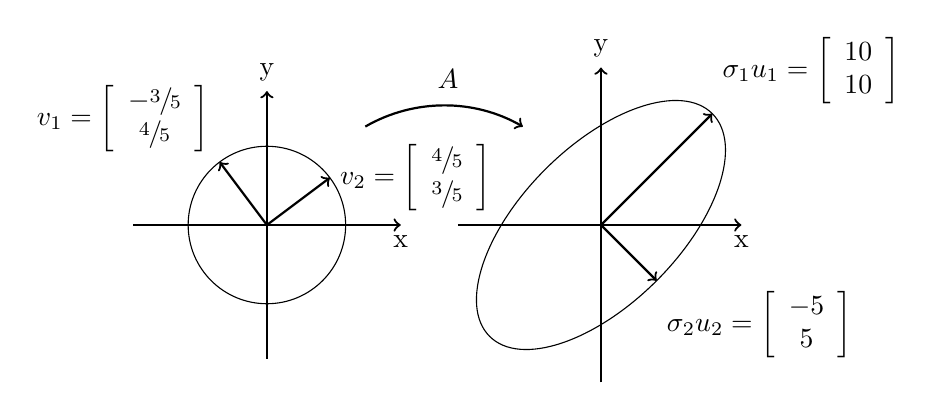
\begin{tikzpicture}
\draw (0,0) circle (1cm);
\draw[rotate=45] (3
,-3) ellipse (2cm and 1cm);

\draw[thick,->] (-1.7,0) -- (1.7,0) node[anchor=north] {x};
\draw[thick,->] (0,-1.7) -- (0,1.7) node[anchor=south] {y};

\draw[thick,->] (2.4264,0) -- (6.0264,0) node[anchor=north ] {x};
\draw[thick,->] (4.24264,-2) -- (4.24264,2) node[anchor=south ] {y};

\draw[thick,->] (0,0) -- (-0.6,0.8) node[anchor=south east] {$v_1=\left[\begin{array}{c}
	-\sfrac{3}{5} \\ 
	\sfrac{4}{5}
	\end{array} \right]$};
\draw[thick,->] (0,0) -- (0.8,0.6) node[anchor= west] {$v_2=\left[\begin{array}{c}
	\sfrac{4}{5} \\ 
	\sfrac{3}{5}
	\end{array} \right]$};

\draw[thick,->] (4.24264,0) -- (5.65685,1.414214) node[anchor=south west] {$\sigma_1u_1=\left[\begin{array}{c}
	10 \\ 
	10
	\end{array} \right]$};
\draw[thick,->] (4.24264,0) -- (4.94975,-0.707106) node[anchor=north west] {$\sigma_2u_2=\left[\begin{array}{c}
	-5 \\ 
	5
	\end{array} \right]$};

\draw[thick,->] (1.25,1.25) arc (120:60:2cm);

\draw (2.3,2.1) node[anchor=north ] {$A$};
\end{tikzpicture}
\end{center}
\item We denote $a_1,a_2$ the columns of $A$ and $a_1^*,a_2^*$ the rows of $A$, we have
\begin{align}
{\left\| A \right\|_1} &= \mathop {\max }\limits_{i = 1,2} {\left\| {{a_i}} \right\|_1} = {\left\| {{a_2}} \right\|_1} = 16\\
{\left\| A \right\|_2} &= \mathop {\max }\limits_{i = 1,2} {\sigma _i} = {\sigma _1} = 10\sqrt 2 \\
{\left\| A \right\|_\infty } &= \mathop {\max }\limits_{i = 1,2} {\left\| {a_i^*} \right\|_1} = {\left\| {a_2^*} \right\|_1} = 15\\
{\left\| A \right\|_F} &= \sqrt {\sigma _1^2 + \sigma _1^2}  = 5\sqrt {10} 
\end{align}
\item We have the SVD
\begin{align}
A=U\Sigma V^T
\end{align}
Therefore,
\begin{align}
{A^{ - 1}} &= {\left( {U\Sigma {V^T}} \right)^{ - 1}}\\
& = {V^{ - T}}{\Sigma ^{ - 1}}{U^{ - 1}}\\
& = V{\Sigma ^{ - 1}}{U^T}\\
& = \left[ {\begin{array}{*{20}{c}}
{\dfrac{1}{{20}}}&{ - \dfrac{{11}}{{100}}}\\
{\dfrac{1}{{10}}}&{ - \dfrac{1}{{50}}}
\end{array}} \right]
\end{align}
\item Use the following \textsc{Matlab} code
\begin{verbatim}
E = eig(A)
\end{verbatim}
yields
\begin{align}
{\lambda _{1,2}} = \dfrac{3}{2} \pm \dfrac{{\sqrt {391} }}{2}i
\end{align}
\item Use the following \textsc{Matlab} code to verify $\det A=\lambda _1 \lambda _2$ and $\left| {\det A} \right| = {\sigma _1}{\sigma _2}$.
\begin{verbatim}
det(A)-E(1)*E(2)
abs(det(A))-10*sqrt(2)*5*sqrt(2)
\end{verbatim}
\item The lengths of the semi-axes of the ellipsoid onto which $A$ maps the unit ball in $\mathbb{R}^2$ are ${\sigma _1} = 10\sqrt 2 ,{\sigma _2} = 5\sqrt 2 $. Therefore, the area of the ellipsoid is 
\begin{align}
{S_{ellipsoid}} = \pi {\sigma _1}{\sigma _2} = 100\pi 
\end{align}
\end{enumerate}
Done. \hfill $\square$\\
\\
\textbf{Problem 1.33 (Exercise 5.4, \cite{1}).} \textit{Suppose $A \in \mathbb{C}^{m\times m}$ has an SVD $A =U\Sigma V^*$. Find an eigenvalue decomposition of the $2m \times 2m$ hermitian martrix}
\begin{align}
M = \left[ {\begin{array}{*{20}{c}}
0&{{A^*}}\\
A&0
\end{array}} \right]
\end{align}
\textsc{Solution 1.} Let $\sigma _i,i=1,2,\ldots,m$ be singular values of $A$. We have
\begin{align}
A{v_i} &= {\sigma _i}{u_i},\hspace{0.5cm} i = 1,2, \ldots ,m\\
{A^*}{u_i} &= {\sigma _i}{v_i},\hspace{0.5cm}  i = 1,2, \ldots ,m
\end{align}
Hence,
\begin{align}
\label{1.12}
\left[ {\begin{array}{*{20}{c}}
0&{{A^*}}\\
A&0
\end{array}} \right]\left[ {\begin{array}{*{20}{c}}
{{v_i}}\\
{{u_i}}
\end{array}} \right] = {\sigma _i}\left[ {\begin{array}{*{20}{c}}
{{v_i}}\\
{{u_i}}
\end{array}} \right]
\end{align}
and
\begin{align}
\label{1.13}
\left[ {\begin{array}{*{20}{c}}
0&{{A^*}}\\
A&0
\end{array}} \right]\left[ {\begin{array}{*{20}{c}}
{{v_i}}\\
{ - {u_i}}
\end{array}} \right] =  - {\sigma _i}\left[ {\begin{array}{*{20}{c}}
{{v_i}}\\
{ - {u_i}}
\end{array}} \right]
\end{align}

Due to \eqref{1.12} and \eqref{1.13}, we have a set of eigenvectors of $M$
\begin{align}
\label{1.14}
\dfrac{1}{{\sqrt 2 }}\left[ {\begin{array}{*{20}{c}}
{  {v_i}}\\
{\pm {u_i}}
\end{array}} \right],i = 1,2, \ldots ,m
\end{align}
corresponding to eigenvalues $\pm \sigma _i$.

We now denote $Q$ the matrix whose columns are the eigenvectors \eqref{1.14} of $M$
\begin{align}
Q = \dfrac{1}{{\sqrt 2 }}\left[ {\begin{array}{*{20}{c}}
V&{  V}\\
U& -U
\end{array}} \right]
\end{align}
Then
\begin{align}
{Q^*} = \left[ {\begin{array}{*{20}{c}}
{{V^*}}&{{U^*}}\\
{ {V^*}}&{-{U^*}}
\end{array}} \right]
\end{align}
and
\begin{align}
Q{Q^*} &= \dfrac{1}{{\sqrt 2 }}\left[ {\begin{array}{*{20}{c}}
V&V\\
U&{ - U}
\end{array}} \right]\dfrac{1}{{\sqrt 2 }}\left[ {\begin{array}{*{20}{c}}
{{V^*}}&{{U^*}}\\
{{V^*}}&{ - {U^*}}
\end{array}} \right]\\
 &= \dfrac{1}{2}\left[ {\begin{array}{*{20}{c}}
{2{I_m}}&0\\
0&{2{I_m}}
\end{array}} \right]\\
& = {I_{2m}}
\end{align}
Thus, $Q$ is invertible and we have an eigenvalue decomposition of $M$ as follow
\begin{align}
M = \dfrac{1}{{\sqrt 2 }}\left[ {\begin{array}{*{20}{c}}
V&V\\
U&{ - U}
\end{array}} \right]\left[ {\begin{array}{*{20}{c}}
\Sigma &0\\
0&{ - \Sigma }
\end{array}} \right]\dfrac{1}{{\sqrt 2 }}{\left[ {\begin{array}{*{20}{c}}
V&V\\
U&{ - U}
\end{array}} \right]^{ - 1}}
\end{align}
\hfill $\square$\\
\\
\textsc{Solution 2.} We consider a SVD of $A$
\begin{align}
A=U\Sigma V^*
\end{align}
We denote $v_i$ the columns of $V$, $u_i$ the columns of $U$ and $\sigma _i$ the singular values of $A$. We want to find eigenvalues and eigenvectors of $M$. The equation
\begin{align}
\left[ {\begin{array}{*{20}{c}}
0&{{A^*}}\\
A&0
\end{array}} \right]\left[ {\begin{array}{*{20}{c}}
{{x_1}}\\
{{x_2}}
\end{array}} \right] = \lambda \left[ {\begin{array}{*{20}{c}}
{{x_1}}\\
{{x_2}}
\end{array}} \right]
\end{align}
yields
\begin{align}
{A^*}{x_2} &= \lambda {x_1}\\
A{x_1} &= \lambda {x_2}
\end{align}
Hence, 
\begin{align}
A{A^*}{x_2} &= \lambda A{x_1}\\
 &= {\lambda ^2}{x_2}
\end{align} 
We deduce that $x_2$ is a left singular vector of $A$.\\

Similarly,
\begin{align}
{A^*}A{x_1} &= \lambda {A^*}{x_2}\\
 &= {\lambda ^2}{x_1}
\end{align}
we deduce that $x_1$ is a right singular vector of $A$. Thus, we obtain $2m$ eigenvectors of $M$ 
\begin{align}
\dfrac{1}{{\sqrt 2 }}\left[ {\begin{array}{*{20}{c}}
{{v_i}}\\
{ \pm {u_i}}
\end{array}} \right],\hspace{0.5cm} i = 1,2, \ldots ,m
\end{align}
corresponding to the eigenvaluess $\lambda =\pm \sigma _i$. Finally, we get the eigenvalue decomposition
\begin{align}
M = \dfrac{1}{{\sqrt 2 }}\left[ {\begin{array}{*{20}{c}}
V&V\\
U&{ - U}
\end{array}} \right]\left[ {\begin{array}{*{20}{c}}
\Sigma &0\\
0&{ - \Sigma }
\end{array}} \right]\dfrac{1}{{\sqrt 2 }}{\left[ {\begin{array}{*{20}{c}}
V&V\\
U&{ - U}
\end{array}} \right]^{ - 1}}
\end{align}
\hfill $\square$\\
\\
\textbf{Problem 1.34.} \textit{Let $A$ be a Hermitian matrix. Prove that there exists an unitary matrix $Q$ such that}
\begin{align}
A=Q\Sigma Q^*
\end{align}
\textsc{Solution.} We consider a SVD of $A$
\begin{align}
A=U\Sigma V^*
\end{align}
Since $A$ is hermitian, all of its singular values of real, therefore
\begin{align}
{A^*} &= V{\Sigma ^*}{U^*}\\
 &= V\Sigma {U^*}
\end{align}
We also have
\begin{align}
{A^2} &= A{A^*}\\
 &= U\Sigma {V^*}V\Sigma {U^*}\\
 &= U{\Sigma ^2}{U^{ - 1}}
\end{align}
Since $\Sigma$ is a diagonal matrix with all positive entries, we can find $A$ by taking the square of $A^2$.
\begin{align}
A &= U\Sigma {U^{ - 1}}\\
 &= U\Sigma {U^*}
\end{align}
Done. \hfill $\square$\\
\chapter{QR Factorization and Least Squares}
\section{Lecture 6: Projectors}
\textbf{Problem 2.1 (Exercise 6.1, \cite{1}).} \textit{If $P$ is an orthogonal projector, then $I-2P$ is unitary. Prove this algebraically, and give a geometric interpretation.}\\
\\
\textsc{Solution.} Since $P$ is an orthogonal projector, we have $P^2=P$ and $P=P^*$. Hence
\begin{align}
{\left( {I - 2P} \right)^*}\left( {I - 2P} \right) &= \left( {I - 2{P^*}} \right)\left( {I - 2P} \right)\\
& = I - 2P - 2{P^*} + 4{P^*}P\\
& = I - 2P - 2P + 4{P^2}\\
& = I - 4P + 4P\\
& = I
\end{align}
Therefore, $I-2P$ is unitary.\\
\\
\textbf{\textsf{Geometric interpretation.}} 
\begin{center}
	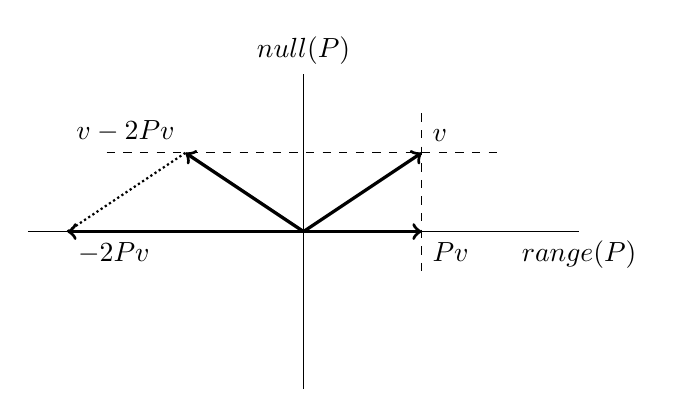
\begin{tikzpicture}
	\draw[very thin,-] (-3.5,0) -- (3.5,0) node[anchor=north] {$range(P)$};
	\draw[very thin,-] (0,-2) -- (0,2) node[anchor=south] {$null(P)$};
	
	\draw[very thick,->] (0,0) -- (1.5,1) node[anchor=south west] {$v$};
	\draw[very thick,->] (0,0) -- (-1.5,1) node[anchor=south east] {$v-2Pv$};
	\draw[very thick,->] (0,0) -- (1.5,0) node[anchor=north west] {$Pv$};
	\draw[very thick,->] (0,0) -- (-3,0) node[anchor= north west] {$-2Pv$};
	
	\draw[thin,dashed] (1.5,1.5) -- (1.5,-0.5);
	\draw[thin,dashed] (-2.5,1) -- (2.5,1);
	\draw[thick,densely dotted] (-1.5,1) -- (-3,0);
	\end{tikzpicture}
\end{center}

From this figure, we see that $I-2P$ is a reflection transform with respect to $null\left(P\right)$. Hence, it keeps the magnitude of any vector $v$, which is consistent which the fact that $I-2P$ is unitary. \hfill $\square$\\
\\
\textbf{Problem 2.2 (Exercise 6.2, \cite{1}).} \textit{Let $E$ be the $m \times m$ matrix that extracts the ``even parts'' of an $m$-vector: $Ex = \dfrac{{x + Fx}}{2}$, where $F$ is the $m \times m$ matrix that flips ${\left( {{x_1}, \ldots ,{x_m}} \right)^*}$ to ${\left( {{x_m}, \ldots ,{x_1}} \right)^*}$. Is $E$ an orthogonal projector, an oblique projector, or not a projector at all? What are its entries?}\\
\\
\textsc{Solution.} The matrix $F$ that flips $\left(x_1,\ldots,x_m\right)^*$ to $\left(x_m,\ldots,x_1\right)^*$ has the form
\begin{align}
F = \left[ {\begin{array}{*{20}{c}}
0&0& \cdots &0&1\\
0&0& \cdots &1&0\\
 \vdots & \vdots & {\mathinner{\mkern2mu\raise1pt\hbox{.}\mkern2mu
 \raise4pt\hbox{.}\mkern2mu\raise7pt\hbox{.}\mkern1mu}} & \vdots & \vdots \\
0&1& \cdots &0&0\\
1&0& \cdots &0&0
\end{array}} \right]
\end{align}
Hence,
\begin{align}
F^* &=F\\
{F^2} &= \left[ {\begin{array}{*{20}{c}}
1&0& \cdots &0&0\\
0&1& \cdots &0&0\\
 \vdots & \vdots & {\mathinner{\mkern2mu\raise1pt\hbox{.}\mkern2mu
 \raise4pt\hbox{.}\mkern2mu\raise7pt\hbox{.}\mkern1mu}} & \vdots & \vdots \\
0&0& \cdots &1&0\\
0&0& \cdots &0&1
\end{array}} \right]\\
& = {I_m}
\end{align}
We have
\begin{align}
\label{1.9}
Ex = \dfrac{{x + Fx}}{2},\forall x \in \mathbb{C}^m
\end{align}
or equivalently,
\begin{align}
E = \dfrac{{{I_m} + F}}{2}
\end{align}
Hence,
\begin{align}
{E^2} &= {\left( {\dfrac{{{I_m} + F}}{2}} \right)^2}\\
& = \dfrac{{{I_m} + 2F + {F^2}}}{4}\\
& = \dfrac{{{I_m} + 2F + {I_m}}}{4}\\
& = \dfrac{{{I_m} + F}}{2}\\
& = E
\end{align}
i.e., $E$ is a projector. 

In addition, we also have
\begin{align}
{E^*} &= {\left( {\dfrac{{{I_m} + F}}{2}} \right)^*}\\
 &= \dfrac{{{I_m^*} + {F^*}}}{2}\\
& = \dfrac{{{I_m} + F}}{2}\\
& = E
\end{align}
i.e., $E$ is an orthogonal projector.

Finally, it is straightforward to compute $E$ explicitly.
\begin{align}
E &= \dfrac{{{I_m} + F}}{2}\\
& = \dfrac{1}{2}\left( {\left[ {\begin{array}{*{20}{c}}
1&0& \cdots &0&0\\
0&1& \cdots &0&0\\
 \vdots & \vdots & {\mathinner{\mkern2mu\raise1pt\hbox{.}\mkern2mu
 \raise4pt\hbox{.}\mkern2mu\raise7pt\hbox{.}\mkern1mu}} & \vdots & \vdots \\
0&0& \cdots &1&0\\
0&0& \cdots &0&1
\end{array}} \right] + \left[ {\begin{array}{*{20}{c}}
0&0& \cdots &0&1\\
0&0& \cdots &1&0\\
 \vdots & \vdots & {\mathinner{\mkern2mu\raise1pt\hbox{.}\mkern2mu
 \raise4pt\hbox{.}\mkern2mu\raise7pt\hbox{.}\mkern1mu}} & \vdots & \vdots \\
0&1& \cdots &0&0\\
1&0& \cdots &0&0
\end{array}} \right]} \right)\\
& = \left\{ {\begin{array}{*{20}{c}}
{\left[ {\begin{array}{*{20}{c}}
{\dfrac{1}{2}}&0& \cdots & \cdots &0&{\dfrac{1}{2}}\\
0& \ddots & \ddots & {\mathinner{\mkern2mu\raise1pt\hbox{.}\mkern2mu
 \raise4pt\hbox{.}\mkern2mu\raise7pt\hbox{.}\mkern1mu}} & {\mathinner{\mkern2mu\raise1pt\hbox{.}\mkern2mu
 \raise4pt\hbox{.}\mkern2mu\raise7pt\hbox{.}\mkern1mu}} &0\\
 \vdots & \ddots &{\dfrac{1}{2}}&{\dfrac{1}{2}}& {\mathinner{\mkern2mu\raise1pt\hbox{.}\mkern2mu
 \raise4pt\hbox{.}\mkern2mu\raise7pt\hbox{.}\mkern1mu}} & \vdots \\
 \vdots & {\mathinner{\mkern2mu\raise1pt\hbox{.}\mkern2mu
 \raise4pt\hbox{.}\mkern2mu\raise7pt\hbox{.}\mkern1mu}} &{\dfrac{1}{2}}&{\dfrac{1}{2}}& \ddots & \vdots \\
0& {\mathinner{\mkern2mu\raise1pt\hbox{.}\mkern2mu
 \raise4pt\hbox{.}\mkern2mu\raise7pt\hbox{.}\mkern1mu}} & {\mathinner{\mkern2mu\raise1pt\hbox{.}\mkern2mu
 \raise4pt\hbox{.}\mkern2mu\raise7pt\hbox{.}\mkern1mu}} & \ddots & \ddots &0\\
{\dfrac{1}{2}}&0& \cdots & \cdots &0&{\dfrac{1}{2}}
\end{array}} \right],\mbox{ if }m\mbox{ is even}}\\
{\left[ {\begin{array}{*{20}{c}}
{\dfrac{1}{2}}&0& \cdots &0&{\dfrac{1}{2}}\\
0& \ddots & \cdots & {\mathinner{\mkern2mu\raise1pt\hbox{.}\mkern2mu
 \raise4pt\hbox{.}\mkern2mu\raise7pt\hbox{.}\mkern1mu}} &0\\
 \vdots & \vdots &1& \vdots & \vdots \\
0& {\mathinner{\mkern2mu\raise1pt\hbox{.}\mkern2mu
 \raise4pt\hbox{.}\mkern2mu\raise7pt\hbox{.}\mkern1mu}} & \cdots & \ddots &0\\
{\dfrac{1}{2}}&0& \cdots &0&{\dfrac{1}{2}}
\end{array}} \right],\mbox{ if } m \mbox{ is odd}}
\end{array}} \right.
\end{align}
Done. \hfill $\square$\\
\\
\textbf{Problem 2.3 (Exercise 6.3, \cite{1}).} \textit{Given $A\in \mathbb{C}^{m\times n}$ with $m \ge n$, show that $A^*A$ is nonsingular if and only if $A$ has full rank.}\\
\\
\textsc{Solution.} Since the nonzero singular values of $A$ are the square roots of the nonzero eigenvalues of $A^*A$, we have that the event $A^*A$ is nonsingular, i.e., $rank\left( {{A^*}A} \right) = n$ and $A^*A$ has $n$ nonzero eigenvalues, is equivalent to the event $A$ has $n$ nonzero singular values, i.e., $rank\left(A\right)=n$ and $A$ has $n$ nonzero singular values, i.e., $A$ has full rank. \hfill $\square$\\
\\
\textbf{Problem 2.4 (Exercise 6.4, \cite{1}).} \textit{Consider the matrices}
\begin{align}
A &= \left[ {\begin{array}{*{20}{c}}
1&0\\
0&1\\
1&0
\end{array}} \right]\\
B &= \left[ {\begin{array}{*{20}{c}}
1&2\\
0&1\\
1&0
\end{array}} \right]
\end{align}
\textit{Answer the following questions by hand calculation.}
\begin{enumerate}
\item \textit{What is the orthogonal projector $P$ onto $range\left(A\right)$, and what is the image under $P$ of the vector $\left(1,2,3\right)^*$?}
\item \textit{Same questions for $B$.}
\end{enumerate}
\textsc{Solution.} 
\begin{enumerate}
\item The orthogonal projector $P_A$ onto $range\left(A\right)$ is
\begin{align}
{P_A}& = A{\left( {{A^*}A} \right)^{ - 1}}{A^*}\\
 &= \left[ {\begin{array}{*{20}{c}}
{\dfrac{1}{2}}&0&{\dfrac{1}{2}}\\
0&1&0\\
{\dfrac{1}{2}}&0&{\dfrac{1}{2}}
\end{array}} \right]
\end{align}

The image under $P_A$ of the vector $v=\left(1,2,3\right)^*$ is
\begin{align}
{P_A}v &= \left[ {\begin{array}{*{20}{c}}
{\dfrac{1}{2}}&0&{\dfrac{1}{2}}\\
0&1&0\\
{\dfrac{1}{2}}&0&{\dfrac{1}{2}}
\end{array}} \right]\left[ {\begin{array}{*{20}{c}}
1\\
2\\
3
\end{array}} \right]\\
& = \left[ {\begin{array}{*{20}{c}}
2\\
2\\
2
\end{array}} \right]
\end{align}
\item Similarly, the orthogonal projector $P_B$ onto $range\left(B\right)$ is
\begin{align}
{P_B} &= B{\left( {{B^*}B} \right)^{ - 1}}{B^*}\\
 &= \left[ {\begin{array}{*{20}{c}}
{\dfrac{5}{6}}&{\dfrac{1}{3}}&{\dfrac{1}{6}}\\
{\dfrac{1}{3}}&{\dfrac{1}{3}}&{ - \dfrac{1}{3}}\\
{\dfrac{1}{6}}&{ - \dfrac{1}{3}}&{\dfrac{5}{6}}
\end{array}} \right]
\end{align}

The image under $P_B$ of the vector $v=\left(1,2,3\right)^*$ is
\begin{align}
{P_B}v &= \left[ {\begin{array}{*{20}{c}}
{\dfrac{5}{6}}&{\dfrac{1}{3}}&{\dfrac{1}{6}}\\
{\dfrac{1}{3}}&{\dfrac{1}{3}}&{ - \dfrac{1}{3}}\\
{\dfrac{1}{6}}&{ - \dfrac{1}{3}}&{\dfrac{5}{6}}
\end{array}} \right]\left[ {\begin{array}{*{20}{c}}
1\\
2\\
3
\end{array}} \right]\\
& = \left[ {\begin{array}{*{20}{c}}
2\\
0\\
2
\end{array}} \right]
\end{align}
\end{enumerate}
Done. \hfill $\square$\\
\\
\textbf{Problem 2.5 (Exercise 6.5, \cite{1}).} \textit{Let $P \in \mathbb{C}^{m\times m}$ be a nonzero projector. Show that ${\left\| P \right\|_2} \ge 1$, with equality if and only if $P$ is an orthogonal projector.}\\
\\
\textsc{Solution.} Since $P$ is an nonzero projector, we have
\begin{align}
\label{1.16}
{\left\| P \right\|_2} = {\left\| {{P^2}} \right\|_2} \le \left\| P \right\|_2^2
\end{align}
Dividing both side of \eqref{1.16} by ${\left\| P \right\|_2} \ne 0$ yields
\begin{align}
\label{1.17}
{\left\| P \right\|_2} \ge 1
\end{align}

We now consider the equality of \eqref{1.17}.
\begin{enumerate}
\item $\left(  \Leftarrow  \right)$ Suppose $P$ is an orthogonal projector, we have 
\begin{align}
{P^2} &= P\\
P &= {P^*}
\end{align}

Since $P$ is hermitian, the singular values of $P$ are the absolute values of the eigenvalues of $P$ (Theorem 5.5, \cite{1}). Hence, 
\begin{align}
\label{1.19}
{\sigma _i} = \left| {{\lambda _i}} \right| \in \left\{ {0,1} \right\},\forall i
\end{align}
Since $P$ is a nonzero projector, there is at least one $\sigma _i =1$, i.e., \eqref{1.19} gives
\begin{align}
{\left\| P \right\|_2} = {\sigma _1} = 1
\end{align}
\item $\left(  \Rightarrow  \right)$ We prove by contradiction. Suppose on the contrary that $P$ is an oblique projector, we need to prove ${\left\| P \right\|_2} > 1$. It suffices to choose an $y$ with ${\left\| y \right\|_2} \le 1$ for which 
\begin{align}
{\left\| {Py} \right\|_2} > {\left\| y \right\|_2}
\end{align}

Since $P$ is an oblique projector, we can choose $u \in range\left( P \right)$ and $v \in null\left( P \right)$ such that 
\begin{align}
{\left\| u \right\|_2} &= 1\\
{\left\| v \right\|_2} &= 1\\
\left\langle {u,v} \right\rangle  &\ne 0 \label{1.24}
\end{align}

(Note that \eqref{1.24} can not hold if $P$ is an orthogonal projector).

We now choose 
\begin{align}
z = u - \left\langle {u,v} \right\rangle v
\end{align}
By \eqref{1.24}, we then have
\begin{align}
\left\| z \right\|_2^2 &= \left\| {u - \left\langle {u,v} \right\rangle v} \right\|_2^2\\
 &= {u^2} - 2\left\langle {u,v} \right\rangle \left\langle {u,v} \right\rangle  + {\left\langle {u,v} \right\rangle ^2}{v^2}\\
& = 1 - {\left\langle {u,v} \right\rangle ^2} < 1
\end{align}
i.e., ${\left\| z \right\|_2} < 1$, whereas
\begin{align}
{\left\| {Pz} \right\|_2} = {\left\| u \right\|_2} = 1
\end{align}

Hence, 
\begin{align}
{\left\| P \right\|_2} &= \mathop {\sup }\limits_{x \in {\mathbb{C}^m},x \ne 0} \dfrac{{{{\left\| {Px} \right\|}_2}}}{{{{\left\| x \right\|}_2}}}\\
 &\ge \dfrac{{{{\left\| {Pz} \right\|}_2}}}{{{{\left\| z \right\|}_2}}}\\
 &= \dfrac{1}{{{{\left\| z \right\|}_2}}} > 1
\end{align}
This contradicts our assumption ${\left\| P \right\|_2} = 1$. Therefore, $P$ is an orthogonal projector.
\end{enumerate}
Done.  \hfill $\square$\\
\section{Lecture 7: QR Factorization}
\textbf{Problem 2.6 (Exercise 7.1, \cite{1}).} \textit{Consider again the matrices $A$ and $B$ of Exercise 6.4, \cite{1}.}
\begin{align}
A &= \left[ {\begin{array}{*{20}{c}}
1&0\\
0&1\\
1&0
\end{array}} \right]\\
B &= \left[ {\begin{array}{*{20}{c}}
1&2\\
0&1\\
1&0
\end{array}} \right]
\end{align}
\begin{enumerate}
\item \textit{Using any method you like, determine (on paper) a reduced QR factorization $A = \hat Q\hat R$ and a full QR factorization $A=QR$.}
\item \textit{Again using any method you like, determine reduced and full QR factorizations $B = \hat Q\hat R$ and $B=QR$.}
\end{enumerate}
\textsc{Solution.} Denote $a_i$ and $b_i$ be the columns of $A$ and $B$ respectively.
\begin{enumerate}
\item \textbf{\textsf{Reduced QR factorization.}}
\begin{align}
A &= \hat Q\hat R\\
{r_{11}} &= {\left\| {{a_1}} \right\|_2} = \sqrt 2 \\
{q_1} &= \dfrac{{{a_1}}}{{{r_{11}}}} = \left[ {\begin{array}{*{20}{c}}
{\dfrac{1}{{\sqrt 2 }}}\\
0\\
{\dfrac{1}{{\sqrt 2 }}}
\end{array}} \right]\\
{r_{12}} &= q_1^*{a_2} = 0\\
{r_{22}} &= {\left\| {{a_2} - {r_{12}}{q_1}} \right\|_2} = 1\\
{q_2} &= \dfrac{{{a_2} - {r_{12}}{q_1}}}{{{r_{22}}}} = \left[ {\begin{array}{*{20}{c}}
0\\
1\\
0
\end{array}} \right]
\end{align}
Hence, 
\begin{align}
A &= \left[ {\begin{array}{*{20}{c}}
1&0\\
0&1\\
1&0
\end{array}} \right]\\
 &= \left[ {\begin{array}{*{20}{c}}
{\dfrac{1}{{\sqrt 2 }}}&0\\
0&1\\
{\dfrac{1}{{\sqrt 2 }}}&0
\end{array}} \right]\left[ {\begin{array}{*{20}{c}}
{\sqrt 2 }&0\\
0&1
\end{array}} \right]
\end{align}
\textbf{\textsf{Full QR factorization.}} 
We take ${a_3} = \left[ {\begin{array}{*{20}{c}}
0\\
0\\
1
\end{array}} \right]$ and find a unit vector $q_3$ orthogonal to $q_1$ and $q_2$.
\begin{align}
{q_3} &= \dfrac{{{a_3} - q_1^*{a_3}{q_1} - q_2^*{a_3}{q_2}}}{{{{\left\| {{a_3} - q_1^*{a_3}{q_1} - q_2^*{a_3}{q_2}} \right\|}_2}}}\\
 &= \left[ {\begin{array}{*{20}{c}}
{ - \dfrac{1}{{\sqrt 2 }}}\\
0\\
{\dfrac{1}{{\sqrt 2 }}}
\end{array}} \right]
\end{align}
Hence, 
\begin{align}
A &= \left[ {\begin{array}{*{20}{c}}
1&0\\
0&1\\
1&0
\end{array}} \right]\\
 &= \left[ {\begin{array}{*{20}{c}}
{\dfrac{1}{{\sqrt 2 }}}&0&{ - \dfrac{1}{{\sqrt 2 }}}\\
0&1&0\\
{\dfrac{1}{{\sqrt 2 }}}&0&{\dfrac{1}{{\sqrt 2 }}}
\end{array}} \right]\left[ {\begin{array}{*{20}{c}}
{\sqrt 2 }&0\\
0&1\\
0&0
\end{array}} \right]
\end{align}
\item \textbf{\textsf{Reduced QR factorization.}}
\begin{align}
{r_{11}} &= {\left\| {{b_1}} \right\|_2} = \sqrt 2 \\
{q_1} &= \dfrac{{{b_1}}}{{{r_{11}}}} = \left[ {\begin{array}{*{20}{c}}
{\dfrac{1}{{\sqrt 2 }}}\\
0\\
{\dfrac{1}{{\sqrt 2 }}}
\end{array}} \right]\\
{r_{12}} &= q_1^*{b_2} = \sqrt 2 \\
{r_{22}} &= {\left\| {{b_2} - {r_{12}}{q_1}} \right\|_2} = \sqrt 3 \\
{q_2} &= \dfrac{{{b_2} - {r_{12}}{q_1}}}{{{r_{22}}}} = \left[ {\begin{array}{*{20}{c}}
{\dfrac{1}{{\sqrt 3 }}}\\
{\dfrac{1}{{\sqrt 3 }}}\\
{ - \dfrac{1}{{\sqrt 3 }}}
\end{array}} \right]
\end{align}
Hence, 
\begin{align}
B &= \left[ {\begin{array}{*{20}{c}}
1&2\\
0&1\\
1&0
\end{array}} \right]\\
 &= \left[ {\begin{array}{*{20}{c}}
{\dfrac{1}{{\sqrt 2 }}}&{\dfrac{1}{{\sqrt 3 }}}\\
0&{\dfrac{1}{{\sqrt 3 }}}\\
{\dfrac{1}{{\sqrt 2 }}}&{ - \dfrac{1}{{\sqrt 3 }}}
\end{array}} \right]\left[ {\begin{array}{*{20}{c}}
{\sqrt 2 }&{\sqrt 2 }\\
0&{\sqrt 3 }
\end{array}} \right]
\end{align}
\textbf{\textsf{Full QR factorization.}} We take ${b_3} = \left[ {\begin{array}{*{20}{c}}
0\\
0\\
1
\end{array}} \right]$ and find a unit vector $q_3$ orthogonal to $q_1$ and $q_2$.
\begin{align}
{q_3} &= \dfrac{{{b_3} - q_1^*{b_3}{q_1} - q_2^*{b_3}{q_2}}}{{{{\left\| {{b_3} - q_1^*{b_3}{q_1} - q_2^*{b_3}{q_2}} \right\|}_2}}}\\
 &= \left[ {\begin{array}{*{20}{c}}
{ - \dfrac{1}{{\sqrt 6 }}}\\
{\dfrac{{\sqrt 6 }}{3}}\\
{\dfrac{1}{{\sqrt 6 }}}
\end{array}} \right]
\end{align}
Hence, 
\begin{align}
B &= \left[ {\begin{array}{*{20}{c}}
1&2\\
0&1\\
1&0
\end{array}} \right]\\
 &= \left[ {\begin{array}{*{20}{c}}
{\dfrac{1}{{\sqrt 2 }}}&{\dfrac{1}{{\sqrt 3 }}}&{ - \dfrac{1}{{\sqrt 6 }}}\\
0&{\dfrac{1}{{\sqrt 3 }}}&{\dfrac{{\sqrt 6 }}{3}}\\
{\dfrac{1}{{\sqrt 2 }}}&{ - \dfrac{1}{{\sqrt 3 }}}&{\dfrac{1}{{\sqrt 6 }}}
\end{array}} \right]\left[ {\begin{array}{*{20}{c}}
{\sqrt 2 }&{\sqrt 2 }\\
0&{\sqrt 3 }\\
0&0
\end{array}} \right]
\end{align}
\end{enumerate}
Done. \hfill $\square$\\
\\
\textbf{Problem 2.7 (Exercise 7.2, \cite{1}).} \textit{Let $A$ be a matrix with the property that columns $1,3,5,7,\ldots$ are orthogonal to columns $2,4,6,8,\ldots$. In a reduced QR factorization $A=\hat Q \hat R$, what special structure does $\hat R$ possess?}\\
\\
\textbf{Problem 2.8 (Exercise 7.3, \cite{1}).} \textit{Let $A$ be an $m\times m$ matrix, and let $a_j$ be its $j$th column. Give an algebraic proof of \textbf{Hadamard's inequality}.}
\begin{align}
\left| {\det A} \right| \le \prod\limits_{j = 1}^m {{{\left\| {{a_j}} \right\|}_2}} 
\end{align}
\textit{Also give a geometric interpretation of this result, making use of the fact that the determinant equals the volume of a parallelepiped.}\\
\\
\textbf{Problem 2.9 (Exercise 7.4, \cite{1}).} \textit{Let ${x^{\left( 1 \right)}},{y^{\left( 1 \right)}},{x^{\left( 2 \right)}}$ and ${y^{\left( 2 \right)}}$ be nonzero vectors in $\mathbb{R}^3$ with the property that $x^{\left(1\right)}$ and $y^{\left(1\right)}$ are linearly independent and so are $x^{\left(2\right)}$ and $y^{\left(2\right)}$. Consider the two planes in $\mathbb{R}^3$,}
\begin{align}
{P^{\left( 1 \right)}} &= \left\langle {{x^{\left( 1 \right)}},{y^{\left( 1 \right)}}} \right\rangle \\
{P^{\left( 2 \right)}} &= \left\langle {{x^{\left( 2 \right)}},{y^{\left( 2 \right)}}} \right\rangle 
\end{align}
\textit{Suppose we wish to find a nonzero vector $v\in \mathbb{R}^3$ that lies in the intersection $P = {P^{\left( 1 \right)}} \cap {P^{\left( 2 \right)}}$. Devise a method for solving this problem by reducing it to the computation of QR factorizations of three $3\times 2$ matrices.}\\
\\
\textbf{Problem 2.10 (Exercise 7.5, \cite{1}).} \textit{Let $A$ be an $m\times n$ matrix ($m \ge n$) and let $A =\hat Q \hat R$ be a reduced QR factorization.}
\begin{enumerate}
\item \textit{Show that $A$ has rank $n$ if and only if all the diagonal entries of $\hat R$ are nonzero.}
\item \textit{Suppose $\hat R$ has $k$ nonzero diagonal entries for some $k$ with $0 \le k < n$. What does this imply about the rank of $A$? Exactly $k$? At most $k$? Give a precise answer, and prove it.}
\end{enumerate}
\textsc{Solution 1.} 
\begin{enumerate}
\item We have the following \textit{rank inequality}.\\
\\
\textbf{Lemma 2.10.1 (Rank Inequality).} \textit{For $A \in {\mathbb{C}^{m \times n}},B \in {\mathbb{C}^{n \times p}}$}
\begin{align}
rank\left( {AB} \right) \le \min \left\{ {rank\left( A \right),rank\left( B \right)} \right\}
\end{align}

Using Lemma 2.10.1 for $\hat Q$ and $\hat R$ yields
\begin{align}
rank\left( A \right) &= rank\left( {\hat Q\hat R} \right)\\
 &\le \min \left\{ {rank\left( {\hat Q} \right),rank\left( {\hat R} \right)} \right\}\\
 &\le n
\end{align}
where the last inequality is deduced from $\hat R \in {C^{n \times n}}$. 

Thus, 
\begin{align}
\label{1.31}
rank\left( A \right) = n \Leftrightarrow rank\left( {\hat R} \right) = n
\end{align}
In addition, $\hat R$ is an upper-triangular matrix. Therefore, \eqref{1.31} means $A$ has rank $n$ if and only if all the diagonal entries of $\hat R$ are nonzero.\\
\\
\textsc{Solution 2.} Since $rank\left( \hat Q\right) =n$, we have
\begin{align}
rank\left( A \right) = rank\left( {\hat Q\hat R} \right) = rank\left( {\hat R} \right)
\end{align}
Therefore, 
\begin{align}
&\hspace{0.5cm} rank\left( A \right) = n\\
& \Leftrightarrow rank\left( {\hat R} \right) = n\\
& \Leftrightarrow \det \left( {\hat R} \right)= \prod\limits_{i = 1}^n {{r_{ii}}}  \ne 0\\
& \Leftrightarrow {r_{ii}} \ne 0,\hspace{0.5cm} i = 1,2, \ldots ,n
\end{align}
\item Since $\hat R$ is an upper-triangular matrix, if it has $k$ nonzero diagonal entries, then it will have at least $k$ linearly indenpendent row vectors. Hence,
\begin{align}
rank\left( A \right) = rank\left( {\hat R} \right) \ge k
\end{align}
\textbf{Example 2.10.2.} 
\begin{align}
A = \left[ {\begin{array}{*{20}{c}}
0&1\\
0&0
\end{array}} \right]
\end{align}
then a reduced QR factorization of $A$ is
\begin{align}
\hat Q &= {I_2}\\
\hat R &= A
\end{align}
We have $k=0$ but $rank\left(A\right)=1>0$.
\end{enumerate}
Done. \hfill $\square$\\
\section{Lecture 8: Gram-Schmidt Orthogonalization}
\textbf{Problem 2.11 (Exercise 8.1, \cite{1}).} \textit{Let $A$ be an $m\times n$ matrix. Determine the exact numbers of floating point additions, subtractions, multiplications, and divisions involved in computing the factorization $A=\hat Q\hat R$ by Algorithm 8.1, \cite{1}.}\\
\\
\textbf{Problem 2.12 (Exercise 8.2, \cite{1}).} \textit{Write a} \textsc{Matlab} \textit{ function \texttt{[Q,R] = mgs(A)} (see Lecture 9, \cite{1}) that computes a reduces QR factorization $A=\hat Q\hat R$ of an $m\times n$ matrix $A$ with $m\ge n$ using modified Gram-Schmidt orthogonalization. The output variables are a matrix $Q\in \mathbb{C}^{m\times n}$ with orthonormal columns and a triangular matrix $R\in \mathbb{C}^{n\times n}$.}\\
\\
\textbf{Problem 2.13 (Exercise 8.3, \cite{1}).} \textit{Each upper-triangular matrix $R_j$ of p. 61, \cite{1} can be interpreted as the product of a diagonal matrix and a unit upper-triangular matrix (i.e., an upper-triangular matrix with 1 on the diagonal). Explain exactly what these factors are, and which line of Algorithm 8.1, \cite{1}, corresponds to each.}
\section{Lecture 9: MATLAB}
\textbf{Problem 2.14 (Exercise 9.1, \cite{1}).} 
\begin{enumerate}
\item \textit{Run the six-line}\textsc{ Matlab}\textit{ program of Experiment 1, \cite{1}, to produce a plot of approximate Legendre polynomials.}
\item \textit{For $k=0,1,2,3$, plot the difference on the 257-point grid between these approximations and the exact polynomials}
\begin{align}
{P_0}\left( x \right) &= 1\\
{P_1}\left( x \right) &= x\\
{P_2}\left( x \right) &= \frac{3}{2}{x^2} - \frac{1}{2}\\
{P_3}\left( x \right) &= \frac{5}{2}{x^3} - \frac{3}{2}x
\end{align}
\textit{How big are the errors, and how are they distributed?}
\item \textit{Compare these results with what you get with grid spacings $\Delta =2^{-\nu}$ for other values of $\nu$. What power of $\Delta x$ appears to control the convergence?}
\end{enumerate}
\textbf{Problem 2.15 (Exercise 9.2, \cite{1}).} \textit{In Experiment 2, the singular values of $A$ match the diagonal elements of a $QR$ factor $R$  approximately. Consider now a very different example. Suppose $Q=I$ and $A=R$, the $m\times m$ matrix (a \textbf{Toeplitz matrix}) with 1 on the main diagonal, 2 on the first superdiagonal, and 0 everywhere else.}
\begin{enumerate}
\item \textit{What are the eigenvalues, determinant, and rank of $A$?}
\item \textit{What is $A^{-1}$?}
\item \textit{Give a nontrivial upper bound on $\sigma _m$, the $m$th singular value of $A$. You are welcome to use}\textsc{Matlab}\textit{ for inspiration, but the bound you give should be justified analytically. (Hint: Use part (2).)}
\end{enumerate}
\textit{This problem illustrates that you cannot always infer much about the singular values of a matrix from its eigenvalues or from the diagonal entries of a QR factor $R$.}\\
\\
\textbf{Problem 2.16 (Exercise 9.3, \cite{1})} 
\begin{enumerate}
\item \textit{Write a}\textsc{Matlab}\textit{ program that sets up a $15\times 40$ matrix with entries 0 everywhere except for the values 1 in the position indicated in the picture below. The upper-leftmost 1 is in position $\left(2,2\right)$, and the lower-rightmost 1 is in position $\left(13,39\right)$. This picture was produced with the command \texttt{spy(A)}}.
\begin{figure}[H]
	\centering
	\includegraphics[scale=0.35]{6}
	\caption{\textit{Exercise 9.3, \cite{1}.}}
\end{figure}
\item \textit{Call \texttt{svd} to compute the singular values of $A$, and prints the results. Plot these numbers using both \texttt{plot} and \texttt{semilogy}. What is the mathematically exact rank of $A$? How does this show up in the computed singular values?}
\item \textit{For each $i$ from 1 to $\mbox{rank}\left(A\right)$, construct the rank-$i$ matrix $B$ that is the best approximation to $A$ in the 2-norm. Use the command \texttt{pcolor(B)} with \texttt{colormap(gray)} to create images of these various approximations.}
\end{enumerate}

\section{Lecture 10: Householder Triangularization}
\textbf{Problem 2.17 (Exercise 10.1, \cite{1}).} \textit{Determine the (1) eigenvalues, (2) determinant and (3) singular values of a Householder reflector. For the eigenvalues, give a geometric argument as well as an algebraic proof.}\\

In the complex case, there is a circle of possible reflections, i.e., the vector $x$ can be reflected to $z\left\| x \right\|{e_1}$, where $z$ is any scalar with $\left| z \right| = 1$. And in the real case, there are two alternatives, with $z =  \pm 1$ in $z\left\| x \right\|{e_1}$. Thus, we just need to handle this problem in the complex case generally. 

Now, in the complex case, suppose we are constructing unitary matrices $Q_k$ in Householder method. Each $Q_k$ is chosen to be a unitary matrix of the form
\begin{align}
{Q_k} = \left[ {\begin{array}{*{20}{c}}
I&0\\
0&F
\end{array}} \right]
\end{align}
where $I$ is the $\left( {k - 1} \right) \times \left( {k - 1} \right)$ identity and $F$ is an $\left( {m - k + 1} \right) \times \left( {m - k + 1} \right)$ unitary matrix.

Suppose, at the beginning of step $k$, the entries $k,\ldots,m$ of the $k$th column are given by the vector $x\in \mathbb{C}^{m-k+1}$. The Householder reflector $F$ effects the following map.
\begin{align}
F:x \mapsto Fx = \left\| x \right\|{e_1}
\end{align}
Explicitly, the Householder reflector $F$ is 
\begin{align}
F = I - 2\dfrac{{v{v^*}}}{{{v^*}v}}
\end{align}
where $v = z\left\| x \right\|{e_1} - x$.\\
\\
\textsc{Solution.} We compute eigenvalues, determinant and singular values of $F$ in turns. First of all, we can easily choose $z$ such that $v \ne 0$.\\
\textbf{1.} If $v^*u=0$, i.e., $u$ is perpendicular to $v$, then 
\begin{align}
Fu &= u - 2v\dfrac{{{v^*}u}}{{{v^*}v}}\\
& = u
\end{align}
Hence, $F$ has $m-k$ eigenvalues 1 since the subspace of $\mathbb{C}^{m-k+1}$ that is orthogonal to $v \ne 0$ has dimension $m-k$.

In addition, we also have $v$ is an eigenvector of $F$ itself. Indeed,
\begin{align}
Fv &= v - 2v\dfrac{{{v^*}v}}{{{v^*}v}}\\
&= v - 2v\\
 &=  - v
\end{align}
Thus, the last eigenvalue of $F$ is $-1$.\\
\\
\textbf{Geometric interpretation.} The reflection of $v$ is $-v$, and reflection of any vector perpendicular to $v$ is $v$ itself.\\
\\
\textbf{2.} The determinant of $F$ is 
\begin{align}
\det F &= \prod\limits_{i = 1}^{m - k + 1} {{\lambda _i}} \\
& = \left( { - 1} \right){1^{m - k}}\\
& =  - 1
\end{align}
\textbf{3.} Since $F$ is unitary, i.e., $F^*F=I$, using the Theorem 5.4, \cite{1}, we deduce that all singular values of $A$ equal to 1. \hfill $\square$\\
\\
\textbf{Problem 2.18 (Exercise 10.2, \cite{1}).} 
\begin{enumerate}
\item \textit{Write a}\textsc{ Matlab}\textit{ function \texttt{[W,R] = house(A)} that computes an implicit representation of a full QR factorization $A=QR$ of an $m\times n$ matrix $A$ with $m\ge n$ using Householder reflections. The output variables are a lower-triangular matrix $W\in \mathbb{C}^{m\times n}$ whose columns are the vectors $v_k$ defining the successive Householder reflections, and a triangular matrix $R\in \mathbb{C}^{n,n}$.}
\item \textit{Write a}\textsc{ Matlab}\textit{ function \texttt{Q = formQ(W)} that takes the matrix $W$ produced by \texttt{house} as input and generates a corresponding $m\times m$ orthogonal matrix $Q$.}
\end{enumerate}
\textbf{Problem 2.19 (Exercise 10.3, \cite{1}).} \textit{Let $Z$ be the matrix}
\begin{align}
Z = \left[ {\begin{array}{*{20}{c}}
1&2&3\\
4&5&6\\
7&8&7\\
4&2&3\\
4&2&2
\end{array}} \right]
\end{align}
\textit{Compute three reduced QR factorizations of $Z$ in}\textsc{ Matlab}\textit{: by the Gram-Schmidt routine \texttt{mgs} of Exercise 8.2, \cite{1}, by the Householder routines \texttt{house} and \texttt{formQ} of Exercise 10.2, \cite{1}, and by}\textsc{ Matlab}\textit{'s built-in command \texttt{[Q,R] = qr(Z,0)}. Compare these three and comment on any differences you see.}\\
\\
\textbf{Problem 2.20 (Exercise 10.4, \cite{1}).} \textit{Consider the $2 \times 2$ orthogonal matrices}
\begin{align}
F& = \left[ {\begin{array}{*{20}{c}}
{ - c}&s\\
s&c
\end{array}} \right]\\
J &= \left[ {\begin{array}{*{20}{c}}
c&s\\
{ - s}&c
\end{array}} \right]
\end{align}
\textit{where $s =\sin \theta _0$ and $c=\cos \theta _0 $ for some $\theta _0$. The first matrix has $\det F=-1$ and is a reflector - the special case of a Householder reflector in dimension 2. The second has  $\det J=1$ and effects a rotation instead of a reflection. Such a matrix is called a \textbf{Givens rotations}.}
\begin{enumerate}
\item \textit{Describe exactly what geometric effects left-multiplications by $F$ and $J$ have on the plane $\mathbb{R}^2$. ($J$ rotates the plane by the angle $\theta$, for example, but is the rotation clockwise or counterclockwise?})
\item \textit{Describe an algorithm for QR factorization that is analogous to Algorithm 10.1, \cite{1}-p.73, but based on Givens rotations instead of Householder reflections.}
\item \textit{Show that your algorithm involves six flops per entry operated on rather than four, so that the asymptotic operation count is 50\% greater than}
\begin{center}
Work for Householder orthogonalization: $\sim 2m{n^2} - \dfrac{2}{3}{n^3}$ flops.
\end{center}
\end{enumerate}
\textsc{Solution 1.} We now solve \textbf{1} and \textbf{2} through trigonometric view points since it is a good idea to use trigonometric in describing geometric effects in \cite{1}.\\ 
\textbf{1.} We consider $\mathbb{R}^2$ in polar coordinate  for simplicity.
\begin{align}
F\left[ {\begin{array}{*{20}{c}}
{r\sin \alpha }\\
{r\cos \alpha }
\end{array}} \right] &= \left[ {\begin{array}{*{20}{c}}
{ - c}&s\\
s&c
\end{array}} \right]\left[ {\begin{array}{*{20}{c}}
{r\sin \alpha }\\
{r\cos \alpha }
\end{array}} \right]\\
& = r\left[ {\begin{array}{*{20}{c}}
{  \sin \theta _0\cos \alpha - \cos \theta _0 \sin \alpha }\\
{\sin \theta _0\sin \alpha  + \cos \theta _0\cos \alpha }
\end{array}} \right]\\
& = \left[ {\begin{array}{*{20}{c}}
{r\sin \left( {\theta _0 - \alpha } \right)}\\
{r\cos \left( {\theta _0 - \alpha } \right)}
\end{array}} \right]
\end{align}
\textbf{Geometric interpretation of $F$.} The left-multiplication by $F$ will reflect the plane $\mathbb{R}^2$ across the hyperplane 
\begin{align}
\theta  = \dfrac{{{\theta _0}}}{2}
\end{align}
We handle $J$ similarly. 
\begin{align}
J\left[ {\begin{array}{*{20}{c}}
{r\sin \alpha }\\
{r\cos \alpha }
\end{array}} \right] &= \left[ {\begin{array}{*{20}{c}}
c&s\\
{ - s}&c
\end{array}} \right]\left[ {\begin{array}{*{20}{c}}
{r\sin \alpha }\\
{r\cos \alpha }
\end{array}} \right]\\
& = r\left[ {\begin{array}{*{20}{c}}
{\cos {\theta _0}\sin \alpha  + \sin {\theta _0}\cos \alpha }\\
{ \cos {\theta _0}\cos \alpha- \sin {\theta _0}\sin \alpha   }
\end{array}} \right]\\
& = \left[ {\begin{array}{*{20}{c}}
{r\sin \left( {\alpha  + {\theta _0}} \right)}\\
{r\cos \left( {\alpha  + {\theta _0}} \right)}
\end{array}} \right]
\end{align}
\textbf{Geometric interpretation of $J$.} The left-multiplication by $F$ will rotate the plane $\mathbb{R}^2$ by the angle $\theta _0$. In particular, if $\theta _0>0$, this rotation is counter-clockwise and if $\theta _0<0$, this rotation is clockwise. Of course, if $\theta _0 =0$ this rotation is identity operator.\\
\\
\textbf{2.} We focus on performing elimination under a single column of $A$, which we then repeat for each column. For Householder, this is done by a single Householder rotation. Since we are using $2\times 2$ rotations, we have to eliminate under a column one number at a time. Given 2-component vector $x = \left[ {\begin{array}{*{20}{c}}
{r\sin \alpha }\\
{r\cos \alpha }
\end{array}} \right]$ , we need 
\begin{align}
\label{1.21}
J:x \mapsto Jx = \left[ {\begin{array}{*{20}{c}}
{{{\left\| x \right\|}_2}}\\
0
\end{array}} \right]
\end{align}
We now use \eqref{1.21} to find givens rotation $J$ explicitly.
\begin{align}
\left[ {\begin{array}{*{20}{c}}
r\\
0
\end{array}} \right] &= J\left[ {\begin{array}{*{20}{c}}
{r\sin \alpha }\\
{r\cos \alpha }
\end{array}} \right]\\
& = \left[ {\begin{array}{*{20}{c}}
{r\sin \left( {\alpha  + {\theta _0}} \right)}\\
{r\cos \left( {\alpha  + {\theta _0}} \right)}
\end{array}} \right]
\end{align}
Thus, we obtain a system of equations
\begin{align}
\label{1.24}
r\sin \left( {\alpha  + {\theta _0}} \right) &= r\\
r\cos \left( {\alpha  + {\theta _0}} \right) &= 0 \label{1.25}
\end{align}
If $r=0$, take $J$ is an arbitrary givens rotations, i.e.,  $\theta _0$ can be taken arbitrarily. If $r \ne 0$, we can choose
\begin{align}
{\theta _0} = \dfrac{\pi }{2} - \alpha 
\end{align}
to make \eqref{1.24}-\eqref{1.25} hold.\\
\\
\textbf{Describe an algorithm for QR factorization for given rotations.} Then we just do this working bottom-up from the column: rotate the bottom two rows to introduce one zero, the the next two rows to introduce a second zero, etc.\\
\\
\textsc{Solution 2.} We now solve \textbf{2} and \textbf{3} as usual. This approach is good for counting flops in \textbf{3}.\\
\textbf{2.} Instead of trigonometric notation, we can take   $x = \left[ {\begin{array}{*{20}{c}}
a\\
b
\end{array}} \right]$ as usual. Then \eqref{1.21} becomes
\begin{align}
\left[ {\begin{array}{*{20}{c}}
{\sqrt {{a^2} + {b^2}} }\\
0
\end{array}} \right]& = J\left[ {\begin{array}{*{20}{c}}
s\\
b
\end{array}} \right]\\
& = \left[ {\begin{array}{*{20}{c}}
{a\cos {\theta _0} + b\sin {\theta _0}}\\
{ - a\sin {\theta _0} + b\cos {\theta _0}}
\end{array}} \right]
\end{align}
Thus, we obtain a system of equations
\begin{align}
\label{1.29}
a\cos {\theta _0} + b\sin {\theta _0} &= \sqrt {{a^2} + {b^2}} \\
 - a\sin {\theta _0} + b\cos {\theta _0} &= 0 \label{1.30}
\end{align}
Solving \eqref{1.29}-\eqref{1.30} out yields
\begin{align}
\cos {\theta _0} &= \dfrac{a}{{\sqrt {{a^2} + {b^2}} }}\\
\sin {\theta _0} &= \dfrac{b}{{\sqrt {{a^2} + {b^2}} }}
\end{align}
Some easy computation yields
\begin{align}
{\tan ^2}{\theta _0} &= \dfrac{1}{{{{\cos }^2}{\theta _0}}} - 1\\
& = \dfrac{{{a^2} + {b^2}}}{{{a^2}}} - 1\\
& = \dfrac{{{b^2}}}{{{a^2}}}
\end{align}
Hence, we can choose
\begin{align}
{\theta _0} = {\arctan \dfrac{b}{a}}
\end{align}
and the description of an algorithm for QR factorization for givens rotations is the same as the above argument.\\
\\
\textbf{3.} To multiply $J$ by a single 2-component vector requires mulplications and 2 addition, or 6 flops, as indicated below
\begin{align}
J\left[ {\begin{array}{*{20}{c}}
a\\
b
\end{array}} \right] = \left[ {\begin{array}{*{20}{c}}
{a \bullet \cos \left( {\arctan \dfrac{b}{a}} \right) \pmb{+} b \bullet \sin \left( {\arctan \dfrac{b}{a}} \right)}\\
{ - a \bullet \sin \left( {\arctan \dfrac{b}{a}} \right) \pmb{+} b \bullet \cos \left( {\arctan \dfrac{b}{a}} \right)}
\end{array}} \right]
\end{align}
That is 6 flops per column vector element of the matrix. Whereas Householder requires 4 flops per column vector element, see \cite{1}-p.59. Therefore, 6 flops of givens rotations is 50\% more than 4 flops of Householder. \hfill $\square$\\
\section{Lecture 11: Least Squares Problems}
\textbf{Problem 2.21 (Exercise 11.1, \cite{1}).} \textit{Suppose the $m\times n$ matrix $A$ has the form}
\begin{align}
A = \left[ {\begin{array}{*{20}{c}}
{{A_1}}\\
{{A_2}}
\end{array}} \right]
\end{align}
\textit{where $A_1$ is a nonsingular matrix of dimension $n\times n$ and $A_2$ is an arbitrary matrix of dimension $\left(m-n\right)\times n$. Prove that}
\begin{align}
{\left\| {{A^ + }} \right\|_2} \le {\left\| {A_1^{ - 1}} \right\|_2}
\end{align}
\textsc{Solution.} Under the orthogonal projector $P \in \mathbb{C}^{m\times m}$ that maps $\mathbb{C}^m$ onto $\mbox{range}\left(A\right)$, any $x\in \mathbb{C}^m$ can be decomposed uniquely as $x=Px+\left(x-Px\right)$, where $Px \in \mbox{range}\left(A\right)$ and $x-Px \in \mbox{null}\left(A\right)$.

Now, we have
\begin{align}
\label{1.3}
{\left( {x - Px} \right)^*}Ay = 0,\forall y \in {\mathbb{C}^n}
\end{align}
since $Ay \in \mbox{range}\left(A\right)$. 

Applying the Hermitian operator on both side of \eqref{1.3} yields
\begin{align}
{y^*}{A^*}\left( {x - Px} \right) = 0,\forall y \in {\mathbb{C}^n}
\end{align}
Hence,
\begin{align}
\label{1.5}
{A^*}\left( {x - Px} \right) = 0
\end{align}
Using \eqref{1.5}, we estimate the 2-norm of the pseudoinverse matrix $A^+$ of $A$ as follow
\begin{align}
{\left\| {{A^ + }} \right\|_2} &= {\sup _{x \in {\mathbb{C}^m},x \ne 0}}\dfrac{{{{\left\| {{A^ + }x} \right\|}_2}}}{{{{\left\| x \right\|}_2}}}\\
& = {\sup _{x \in {\mathbb{C}^m},x \ne 0}}\dfrac{{{{\left\| {{{\left( {{A^*}A} \right)}^{ - 1}}{A^*}\left( {Px + \left( {x - Px} \right)} \right)} \right\|}_2}}}{{{{\left\| {Px + \left( {x - Px} \right)} \right\|}_2}}}\\
& \le {\sup _{x \in {\mathbb{C}^m},x \ne 0}}\dfrac{{{{\left\| {{{\left( {{A^*}A} \right)}^{ - 1}}{A^*}Px} \right\|}_2}}}{{{{\left\| {Px} \right\|}_2}}}\\
& = {\sup _{y \in {\mathbb{C}^m},y \ne 0}}\dfrac{{{{\left\| {{{\left( {{A^*}A} \right)}^{ - 1}}{A^*}Ay} \right\|}_2}}}{{{{\left\| {Ay} \right\|}_2}}} \label{1.9}\\
& = {\sup _{y \in {\mathbb{C}^m},y \ne 0}}\dfrac{{{{\left\| y \right\|}_2}}}{{{{\left\| {Ay} \right\|}_2}}}\\
& \le {\sup _{y \in {\mathbb{C}^m},y \ne 0}}\dfrac{{{{\left\| y \right\|}_2}}}{{\sqrt {\left\| {{A_1}y} \right\|_2^2 + \left\| {{A_2}y} \right\|_2^2} }}\\
& \le {\sup _{y \in {\mathbb{C}^m},y \ne 0}}\dfrac{{{{\left\| y \right\|}_2}}}{{{{\left\| {{A_1}y} \right\|}_2}}}\\
& = {\sup _{y \in {\mathbb{C}^m},y \ne 0}}\dfrac{{{{\left\| {A_1^{ - 1}y} \right\|}_2}}}{{{{\left\| y \right\|}_2}}}\\
& = \left\| {A_1^{ - 1}} \right\|_2^2
\end{align}
where the equality \eqref{1.9} is deduced from the fact that there exists an nonzero vector $y \in \mathbb{C}^n$ such that $Px=Ay$ since $Px \in \mbox{range}\left(A\right)$.

We also have used the following estimate
\begin{align}
\label{1.12}
\left\| {Px + \left( {x - Px} \right)} \right\|_2^2 &= \left\| {Px} \right\|_2^2 + \left\| {x - Px} \right\|_2^2\\
 &\ge \left\| {Px} \right\|_2^2 \label{1.13}
\end{align}
The estimate \eqref{1.12}-\eqref{1.13} is deduce from applying the Pythagorean theorem for two orthogonal vector $Px \bot \left( {x - Px} \right)$. Done. \hfill $\square$\\
\\
\textbf{Problem 2.22 (Exercise 11.2, \cite{1}).}
\begin{enumerate}
\item \textit{How closely, as measured in the $L^2$ norm on the interval $\left[1,2\right]$, can the function $f\left(x\right)=x^{-1}$ be fitted by a linear combination of the function $e^x, \sin x$ and $\Gamma \left(x\right)$? ($\Gamma \left(x\right)$ is the gamma function, a built-in function in \textsc{Matlab}.) Write a program that determines the answer to at least two digits of relative accuracy using the discretization of $\left[1,2\right]$ and a discrete least squares problem. Write down your estimate of the answer and also of the coefficients of the optimal linear combination, and produce a plot of the optimal approximation.}
\item \textit{Now repeat, but with $\left[1,2\right]$ replaced by $\left[0,1\right]$, You may find the following fact helpful: if $g\left( x \right) = \dfrac{1}{{\Gamma \left( x \right)}}$ then $g'\left( 0 \right) = 1$.}
\end{enumerate}
\textsc{Solution.} 
\begin{enumerate}
\item Using the following \textsc{Matlab} code
\begin{verbatim}
close all
clear all
clc
format long

% Trefethen & Bau, Exercise 11.2.
N = 300;
for n = 2:N
   % set up least square problem.
   A = zeros(n,3);
   x = linspace(1,2,n);
   A(:,1) = exp(x');
   A(:,2) = sin(x');
   A(:,3) = gamma(x');
   b = 1./x';
   % solve least square problem.
   [Q,R] = qr(A);
   sol = R\(Q'*b);
   % compute L^2 norm of error.
   error(n) = sqrt(quad(@(z)F(z,sol(1),sol(2),sol(3)),1,2));
   % compute discrete L^2 norm of error.
   discrete_error(n) = sqrt((norm(b-sol(1)*A(:,1)- ...
                       sol(2)*A(:,2)-sol(3)*A(:,3)))^2/n);
end
plot(2:N,error(2:N),2:N,discrete_error(2:N));
xlabel('Number of Data Points');
ylabel('Errors');
title('Errors of Least Square Problems');
legend('L^2 norm','discrete L^2 norm');
print('-r300','-djpeg');
\end{verbatim}
and subroutine
\begin{verbatim}
function y = F(z,c1,c2,c3)
y = (1./z-c1*exp(z)-c2*sin(z)-c3*gamma(z)).^2;
\end{verbatim}
yields 
\begin{figure}[H]
	\centering
	\includegraphics[scale=0.14]{1}
	\caption{\textit{The $L^2$ norm of error on the interval $\left[1,2\right]$.}}
\end{figure}
\item Using the following \textsc{Matlab} code
\begin{verbatim}
close all
clear all
clc
format long

% Trefethen & Bau, Exercise 11.2.
N = 200;
tol = 1e-13;
for n = 2:N
   % set up least square problem.
   A = zeros(n,3);
   x = linspace(tol,1,n);
   A(:,1) = exp(x');
   A(:,2) = sin(x');
   A(:,3) = gamma(x');
   b = 1./x';
   % solve least square problem.
   [Q,R] = qr(A);
   sol = R\(Q'*b);
   % compute L^2 norm of error.
   error(n) = sqrt(quad(@(z)F(z,sol(1),sol(2),sol(3)),tol,1));
   % compute discrete L^2 norm of error.
   discrete_error(n) = sqrt((norm(b-sol(1)*A(:,1)- ...
                       sol(2)*A(:,2)-sol(3)*A(:,3)))^2/n);
end
plot(2:N,error(2:N),2:N,discrete_error(2:N));
xlabel('Number of Data Points');
ylabel('Errors');
title('Errors of Least Square Problems');
legend('L^2 norm','discrete L^2 norm');
print('-r300','-djpeg');
\end{verbatim}
and subroutine
\begin{verbatim}
function y = F(z,c1,c2,c3)
y = (1./z-c1*exp(z)-c2*sin(z)-c3*gamma(z)).^2;
\end{verbatim}
yields
\begin{figure}[H]
	\centering
	\includegraphics[scale=0.14]{2}
	\caption{\textit{The $L^2$ norm of error on the interval $\left[10^{-13},1\right]$.}}
\end{figure}
If you use \texttt{tol=1e-14}, this \textsc{Matlab} code returns
\begin{figure}[H]
	\centering
	\includegraphics[scale=0.14]{3}
	\caption{\textit{The $L^2$ norm of error on the interval $\left[10^{-14},1\right]$.}}
\end{figure}
If you use \texttt{tol=1e-15}, this \textsc{Matlab} code returns
\begin{figure}[H]
	\centering
	\includegraphics[scale=0.14]{4}
	\caption{\textit{The $L^2$ norm of error on the interval $\left[10^{-15},1\right]$.}}
\end{figure}
If you use \texttt{tol=1e-16}, this \textsc{Matlab} code returns
\begin{figure}[H]
	\centering
	\includegraphics[scale=0.14]{5}
	\caption{\textit{The $L^2$ norm of error on the interval $\left[10^{-16},1\right]$.}}
\end{figure}
\end{enumerate}
Done. \hfill $\square$\\
\\
\textbf{Problem 2.23 (Exercise 11.3, \cite{1}).} \textit{Take $m=50,n=12$. Using}\textsc{ Matlab}\textit{'s \texttt{linspace}, define $t$ to be the $m$-vector corresponding to linearly spaced grid points from 0 to 1. Using}\textsc{ Matlab}\textit{'s \texttt{vander} and \texttt{fliplr}, define $A$ to be the $m\times n$ matrix associated with least squares fitting on this grid by a polynomial of degree $n-1$. Take $b$ to the function $\cos \left(4t\right)$ evaluated on the grid. How, calculate and print (to sixteen-digit precision) the least squares coefficients vector $x$ by six methods:}
\begin{enumerate}
\item \textit{Formation and solution of the normal equations, using}\textsc{ Matlab}\textit{'s}\verb|\|.
\item \textit{$QR$ factorization computed by \texttt{mgs} (modified Gram-Schmidt, Exercise 8.2, \cite{1}).}
\item \textit{$QR$ factorization computed by \texttt{house} (Householder triangularization, Exercise 10.2, \cite{2}).}
\item \textit{$QR$ factorization computed by}\textsc{ Matlab}\textit{'s \texttt{qr} (also Householder triangularization).}
\item \verb|x = A\b|\textit{ in}\textsc{ Matlab}\textit{ (also based on $QR$ factorization).}
\item \textit{SVD, using}\textsc{ Matlab}\textit{'s \texttt{svd}}.
\item \textit{The calculations above will produce six lists of twelve coefficients. In each list, shade with red pen the digits that appear to be wrong (affected by rounding error). Comment on what differences you observe. Do the normal equations exhibit instability? You do not have to explain your observations.}
\end{enumerate}





\chapter{Conditioning and Stability}
\section{Lecture 12: Conditioning and Condition Numbers}
\textbf{Problem 3.1 (Exercise 12.1, \cite{1}).} \textit{Suppose $A$ is a $202\times 202$ matrix with ${\left\| A \right\|_2} = 100$ and ${\left\| A \right\|_F} = 101$. Give the sharpest possible lower bound on the 2-norm condition number $\kappa \left(A\right)$.}\\
\\
\textbf{Problem 3.2 (Exercise 12.2, \cite{1}).} \textit{In Example 11.1, \cite{1}, we remarked that polynomial interpolation in equispaced points is ill-conditioned. To illustrate this phenomenon, let $x_1,\ldots,x_n$ and $y_1,\ldots,y_m$ be $n$ and $m$ equispaced points from $-1$ to 1, respectively.}
\begin{enumerate}
\item \textit{Derive a formula for the $m\times n$ matrix $A$ that maps an $n$-vector of data at $\left\{ {{x_j}} \right\}$ to an $m$-vector of sampled values $\left\{ {p\left( {{y_j}} \right)} \right\}$, where $p$ is the degree $n-1$ polynomial interpolant of the data (see Example 1.1, \cite{1}).} 
\item \textit{Write a program to calculate $A$ and plot ${\left\| A \right\|_\infty }$ on a semilog scale for $n=1,2,\ldots,30,m=2n-1$. In the continuous limit $m\to \infty$, the number ${\left\| A \right\|_\infty }$ are known as the \textbf{Lebesgue constants} for equispaced interpolation, which are asymptotic to}
\begin{align}
\frac{{{2^n}}}{{e\left( {n - 1} \right)\log n}}
\end{align}
\textit{as $n \to \infty$.}
\item \textit{For $n=1,2,\ldots,30$ and $m=2n-1$, what is the $\infty$-norm condition number $\kappa$ of the problem of interpolating the constant function 1? Use}
\begin{align}
\kappa  = \frac{{\left\| {J\left( x \right)} \right\|\left\| x \right\|}}{{\left\| {f\left( x \right)} \right\|}}
\end{align}
\item \textit{How close is your result for $n=11$ to the bound implicit in the following Figure.} 
\end{enumerate}
\begin{figure}[H]
	\centering
	\includegraphics[scale=0.35]{7}
	\caption{\textit{Degree 10 polynomial interpolant to eleven data points. The axis scales are not given, as these have no effect on the picture.}}
\end{figure}
\textbf{Problem 3.3 (Exercise 12.3, \cite{1}).} \textit{The goal of this problem is to explore some properties of random matrices. Your job is to be a laboratory scientist, performing experiments that lead to conjectures and more refined experiments. Do not try to prove any thing. Do produce well-designed plots, which are worth a thousand numbers.}

\textit{Define a \textbf{random matrix} to be an $m\times m$ matrix whose entries are independent samples from the real normal distribution with mean zero and standard derivation $\frac{1}{{\sqrt m }}$. (In}\textsc{ Matlab}\textit{, \texttt{A = randn(m,m)/sqrt(m)}.) The factor $\sqrt m$ is introduced to make the limiting behavior clean as $m\to \infty$.}
\begin{enumerate}
\item \textit{What do the eigenvalues of a random matrix look like? What happens, say, if you take 100 random matrices and superimpose all their eigenvalues in a single plot? If you do this for $m=8,16,32,64,\ldots$, what pattern is suggested? How does the spectral radius $\rho \left(A\right)$ (Exercise 3.2, \cite{1}) behave as $m\to \infty$?}
\item \textit{What about norms? How does the 2-norm of a random matrix behave as $m\to \infty$? Of course, we must have $\rho \left( A \right) \le \left\| A \right\|$ (Exercise 3.2, \cite{1}). Does this inequality appear to approach an equality as $m\to \infty$?}
\item \textit{What about condition numbers-or more simply, the smallest singular value $\sigma _{\min}$? Even for fixed $m$ this equation is interesting. What proportions of random matrices in $\mathbb{R}^{m\times
 m}$ seem to have ${\sigma _{\min }} \le \frac{1}{2},\frac{1}{4},\frac{1}{8}, \ldots $? In other words, what does the tail of the probability distribution of smallest singular values look like? How does the scale of all this change with $m$?}
\item \textit{How do the answer to (1)-(3) change if we consider random triangular instead of full matrices, i.e., upper-triangular matrices whose entries are samples from the same  distribution as above?}
\end{enumerate}




\section{Lecture 13: Floating Point Arithmetic}
\textbf{Problem 3.4 (Exercise 13.1, \cite{1}).} \textit{Between an adjacent pair of nonzero IEEE single precision real numbers, how many IEEE double precision numbers are there?}\\
\\
\textbf{Problem 3.5 (Exercise 13.2, \cite{1}).} \textit{The floating point system $\mathbb{F}$ defined by}
\begin{align}
x =  \pm \left( {m/{\beta ^t}} \right){\beta ^e}
\end{align}
\textit{includes many integers, but not all of them.}
\begin{enumerate}
\item \textit{Give an exact formula for the smallest positive integer $n$ that does not belong to $\mathbb{F}$.}
\item \textit{In particular, what are the values of $n$ for IEEE single and double precision arithmetic?}
\item \textit{Figure out a way to verify this result for your own computer. Specifically, design and run a program that produces evidence that $n-3,n-2$, and $n-1$ belong to $\mathbb{F}$ but $n$ does not. What about $n+1,n+2,n+3$?}
\end{enumerate}
\textbf{Problem 3.6 (Exercise 13.3, \cite{1}).} \textit{Consider the polynomial}
\begin{align}
p\left( x \right)& = {\left( {x - 2} \right)^9}\\
& = {x^9} - 18{x^8} + 144{x^7} - 672{x^6} + 2016{x^5} - 4032{x^4}\\
& + 5376{x^3} - 4608{x^2} + 2304x - 512
\end{align}
\begin{enumerate}
\item \textit{Plot $p\left(x\right)$ for $x=-1.920,-1.919,-1.918,\ldots,2.080$, evaluating $p$ via its coefficients $1,-18,144,\ldots$.}
\item \textit{Produce the same plot again, now evaluating $p$ via the expression $\left(x-2\right)^9$.}
\end{enumerate}
\textbf{Problem 3.7 (Exercise 13.4, \cite{1}).} \textit{The polynomial $p\left(x\right)=x^5-2x^4-3x^3+3x^2-2x-1$ has three real zeros. Applying Newton's method to $p$ with initial guess $x_0=0$ produces a series of estimates $x_1,x_2,x_3,\ldots$ that converge rapidly to a zero $x_* \approx -0.315$.}
\begin{enumerate}
\item \textit{Compute $x_1,\ldots,x_6$ in floating point arithmetic with $\epsilon _{\mbox{machine}}\approx 10^{-16}$. How many digits do you estimate are correct in each of these numbers?}
\item \textit{Compute $x_1,\ldots,x_6$ again exactly with the aid of a symbolic algebra system such as}\textsc{ Maple}\textit{ or}\textsc{Mathematica}.\textit{ Each $x_j$ is a rational number. How many digits are there in the numerator and the denominator for each $j$?}
\end{enumerate}



\section{Lecture 14: Stability}
\textbf{Problem 3.8 (Exercise 14.1, \cite{1}).} \textit{True of False?}
\begin{enumerate}
\item $\sin x = O\left( 1 \right)$ \textit{as} $x \to \infty $.
\item $\sin x = O\left( 1 \right)$ \textit{as} $x \to 0 $.
\item $\log x = O\left( {{x^{\frac{1}{{100}}}}} \right)$ \textit{as} $x \to \infty $.
\item $n! = O\left( {{{\left( {\frac{n}{e}} \right)}^n}} \right)$ \textit{as} $n \to \infty $.
\item \textit{$A = O\left( {{V^{\frac{2}{3}}}} \right)$ as $V \to \infty $, where $A$ and $V$ are the surface area and volume of a sphere measured in square miles and cubic microns, respectively.}
\item $fl\left( \pi  \right) - \pi  = O\left( {{\epsilon _{machine}}} \right)$. \textit{(We dot not mention that the limit is $\epsilon _{machine} \to 0$, since that is implicit for all expressions $O\left(\epsilon _{machine}\right)$ in this book.}
\item $fl\left( {n\pi } \right) - n\pi  = O\left( {{\epsilon _{machine}}} \right)$\textit{, uniformly for all integers $n$. (Here $n\pi$ represents the exact mathematical quantity, not the result of a floating point calculation.}
\end{enumerate}
\textbf{Problem 3.9 (Exercise 14.2, \cite{1}).}
\begin{enumerate}
\item \textit{Show that}
\begin{align}
\left( {1 + O\left( {{\epsilon _{machine}}} \right)} \right)\left( {1 + O\left( {{\epsilon _{machine}}} \right)} \right) = 1 + O\left( {{\epsilon _{machine}}} \right)
\end{align}
\textit{The precise meaning of this statement is that if $f$ is a function satisfying }
\begin{align}
f\left( {{\epsilon _{machine}}} \right) = \left( {1 + O\left( {{\epsilon _{machine}}} \right)} \right)\left( {1 + O\left( {{\epsilon _{machine}}} \right)} \right)\mbox{ as } {\epsilon _{machine}} \to 0
\end{align}
\textit{then $f$ also satisfies}
\begin{align}
f\left( {{\epsilon _{machine}}} \right) = 1 + O\left( {{\epsilon _{machine}}} \right)\mbox{ as } {\epsilon _{machine}} \to 0
\end{align}
\item \textit{Show that}
\begin{align}
{\left( {1 + O\left( {{\epsilon _{machine}}} \right)} \right)^{ - 1}} = 1 + O\left( {{\epsilon _{machine}}} \right)
\end{align}
\end{enumerate}


\section{Lecture 15: More on Stability}
\textbf{Problem 3.10 (Exercise 15.1, \cite{1}).} \textit{Each of the following problems describes an algorithm implemented on a computer satisfying the axioms}\\
\textbf{Axiom 3.10.1.}
\begin{align}
\label{3.11}
\forall x \in \mathbb{R},\exists \epsilon ,\left| \epsilon  \right| \le {\epsilon _{machine}},fl\left( x \right) = x\left( {1 + \epsilon } \right)
\end{align}
\textbf{Fundamental Axiom of Floating Point Arithmetic 3.10.2.}
\begin{align}
\label{3.12}
\forall x \in F,\forall y \in F,\exists \epsilon ,\left| \epsilon  \right| \le {\epsilon _{machine}},x \raisebox{.3pt}{\textcircled{\raisebox{-3pt} {*}}}  y = \left( {x * y} \right)\left( {1 + \epsilon } \right)
\end{align}
\textit{For each one, state whether the algorithm is \textbf{backward stable, stable but not backward stable} or \textbf{unstable}, and prove it or at least give a reasonably convincing argument. Be sure to follow the definitions as given in the text.}
\begin{enumerate}
\item \textit{Data: $x\in \mathbb{C}$. Solution: $2x$, computed as $x \oplus x$.}
\item \textit{Data: $x\in \mathbb{C}$. Solution: $x^2$, computed as $x \otimes x$.}
\item \textit{Data: $x \in \mathbb{C}\backslash \left\{ 0 \right\}$. Solution: 1, computed as} $x$ \encircle{$\div$ }$\ x$.\textit{ (A machine satisfying}
\begin{align}
x \raisebox{.3pt}{\textcircled{\raisebox{-3pt} {*}}}  y = fl\left(x*y\right)
\end{align}
\textit{will give exactly the right answer, but our definitions are based on the weaker condition \eqref{3.12}.)}
\item \textit{Data: $x\in \mathbb{C}$. Solution: 0,  computed as $x \raisebox{.3pt}{\textcircled{\raisebox{-3pt} {-}}}$. (Again, a real machine may do better than our definitions based on \eqref{3.12}.)}
\item \textit{Data: none. Solution: $e$, computed by summing $\sum\nolimits_{k = 0}^\infty  {\frac{1}{{k!}}} $ from left to right using $ \otimes$ and $\oplus $, stopping when a summand is reached of magnitude $<\epsilon _{machine}$.}
\item \textit{Data: none. Solution: $e$, computed by the same algorithm as above except with the series summed from right to left.}
\item \textit{Data: none. Solution: $\pi$, computed by doing an exhaustive search to find the smallest floating point number $x$ in the interval $\left[3,4\right]$ such that}
\begin{align}
s\left( x \right) \otimes s\left( {x'} \right) \le 0
\end{align}
\textit{Here $s\left(x\right)$  is an algorithm that calculates $\sin x$ stably in the given interval, and $x'$ denotes  the next floating point number after $x$ in the floating point system.}
\end{enumerate}
\textbf{Problem 3.11 (Exercise 15.2, \cite{1}).} \textit{Consider an algorithm for the problem of computing the (full) SVD of a matrix. The data for this problem is a matrix $A$, and the solution is three matrices $U$ (unitary), $\sum$ (diagonal), and $V$ (unitary) such that $A=U\sum V^*$. (We are speaking here of explicit matrices $U$ and $V$, not implicit representations as products of reflectors.)}
\begin{enumerate}
\item \textit{Explain what it would mean for this algorithm to be backward stable.}
\item \textit{In fact, for a simple reason, this algorithm cannot be backward stable. Explain.}
\item \textit{Fortunately, the standard algorithms for computing the SVD (Lecture 31, \cite{1}) are stable. Explain what stability means for such an algorithm.}
\end{enumerate}




\section{Lecture 16: Stability of Householder Triangularization}
\textbf{Problem 3.12 (Exercise 16.1, \cite{1}).}
\begin{enumerate}
\item \textit{Let unitary matrices $Q_1,\ldots,Q_k \in \mathbb{C}^{m,m}$ be fixed and consider the problem of computing, for $A\in \mathbb{C}^{m\times n}$, the product $B=Q_k \ldots Q_1 A$. Let the computation be carried out from right to left by straightforward floating point operations on a computer satisfying \eqref{3.11} and \eqref{3.12}. Show that this algorithm is backward stable. (Here $A$ is thought of as data that can be perturbed; the matrices $Q_j$ are fixed and not to be perturbed.)}
\item \textit{Give an example to show that this result no longer holds if the unitary matrices $Q_j$ are replaced by arbitrary matrices $X_j \in \mathbb{C}^{m\times m}$.}
\end{enumerate}
\textbf{Problem 3.13 (Exercise 16.2, \cite{1}).} \textit{The idea of this exercise is to carry out an experiment analogous to the one described in this lecture, but for the SVD instead of $QR$ factorization.}
\begin{enumerate}
\item \textit{Write a}\textsc{ Matlab}\textit{ program that constructs a $50\times 50$ matrix \texttt{A = U*S*V'}, where $U$ and $V$ are random orthogonal matrices and $S$ is a diagonal matrix whose diagonal entries are random uniformly distributed numbers in $\left[0,1\right]$, sorted into nonincreasing order. Have your program compute \texttt{[U2,S2,V2] = svd(A)} and the norms of \texttt{U-U2, V-V2, S-S2}, and \texttt{A-U2*S2*V2'}. Do this for five matrices $A$ and comment on the results. (Hint: Plots of \texttt{diag(U2'*U)} and \texttt{diag(V2'*V)} may be informative.}
\item \textit{Fix the signs in your computed SVD so that the difficulties of (1) go away. Run the program again for five random matrices and comment on the various norms. Do they have a connection with \texttt{cond(A)}?}
\item \textit{Replace the diagonal entries of $S$ by their sixth powers and repeat (2). Do you see significant differences between the results of this exercise and those of the experiments for $QR$ factorization?}
\end{enumerate}




\section{Lecture 17: Stability of Back Substitution}
\textbf{Problem 3.14 (Exercise 17.1, \cite{1}).} \textit{For any particular choice of norm $\left\|  \cdot  \right\|$, the bound}
\begin{align}
\frac{{\left| {\delta {r_{ij}}} \right|}}{{\left| {{r_{ij}}} \right|}} \le m{\epsilon _{machine}} + O\left( {\epsilon _{machine}^2} \right)
\end{align}
\textit{implies a more quantitative normwise bound than}
\begin{align}
\frac{{\left\| {\delta R} \right\|}}{{\left\| R \right\|}} = O\left( {{\epsilon _{machine}}} \right)
\end{align}
\textit{Derive such bounds for the norms ${\left\|  \cdot  \right\|_1}$, ${\left\|  \cdot  \right\|_2}$ and ${\left\|  \cdot  \right\|_\infty}$.}\\
\\
\textbf{Problem 3.15 (Exercise 17.2, \cite{1}).}  \textit{Let $L\in \mathbb{C}^{m\times m}$ be a unit lower-triangular matrix (i.e., with diagonal entries equal to 1). For convenience, write $L$ in the form}
\begin{align}
sL = \left[ {\begin{array}{*{20}{c}}
1&{}&{}&{}&{}\\
{ - {l_{2,1}}}&1&{}&{}&{}\\
{ - {l_{3,1}}}&{ - {l_{3,2}}}&1&{}&{}\\
 \vdots & \vdots &{}& \ddots &{}\\
{ - {l_{m,1}}}&{ - {l_{m,2}}}&{ - {l_{m,3}}}& \cdots &1
\end{array}} \right]
\end{align}
\textit{and define $M=L^{-1}$.}
\begin{enumerate}
\item \textit{Derive a formula for $m_{ij}$ (which may involve other entries of $M$). Which entries of $L$ does $m_{ij}$ depend on?}
\item \textit{Suppose the subdiagonal entries of $L$ are independent random numbers $\pm 1$ with equal probability. Fix $k$ and define}
\begin{align}
{\mu _1} &= {m_{kk}}\\
{\mu _2} &= {m_{k + 1,k}}\\
{\mu _3} &= {m_{k + 2,k}}\\
 &\cdots 
\end{align}
\textit{Write down a system of recurrences relations with random coefficients for the numbers $\mu _j$.}
\item \textit{Experiments show that random triangular matrices with entries $\pm 1$ are exponentially ill-conditioned in the sense that if $\kappa _m$ denote the 2-norm condition number of a matrix of this kind of dimension $m$, then}
\begin{align}
\mathop {\lim }\limits_{m \to \infty } \sqrt[m]{{{\kappa _m}}} = C
\end{align}
\textit{for some constant $1<C<1.5$. (The limit process can be made precise in various ways, but we shall not go into the technicalities; think of it as holding ``with probability 1.'') Perform numerical experiments involving random matrices of various dimensions to estimate $C$ to 10\% accuracy of better.}
\item \textit{Larger scale experiments become feasible if the random matrices of (3) are replaced by the random sequences $\mu _1,\mu_2,\mu _3,\ldots $ of (2). Explain (without proof) why the constant $C$ can also be obtained by considering these sequences, and carry out numerical experiments to estimate $C$ to 1\% accuracy or better.}
\end{enumerate}

\section{Lecture 18: Conditioning of Least Squares Problems}
\textbf{Problem 3.16 (Exercise 18.1, \cite{1}).} \textit{Consider the example}
\begin{align}
A& = \left[ {\begin{array}{*{20}{c}}
1&1\\
1&{1.0001}\\
1&{1.0001}
\end{array}} \right]\\
b& = \left[ {\begin{array}{*{20}{c}}
2\\
{0.0001}\\
{4.0001}
\end{array}} \right]
\end{align}
\begin{enumerate}
\item \textit{What are the matrices $A^+$ and $P$ for this example? Give exact answers.}
\item \textit{Find the exact solutions $x$ and $y=Ax$ to the least squares problem $Ax\approx b$.}
\item \textit{What are $\kappa \left(A\right),\theta$, and $\eta$? From here on, numerical answers are acceptable.}
\item \textit{What are the four condition numbers of Theorem 18.1, \cite{1}?}
\item \textit{Give examples of perturbations $\delta b$ and $\delta A$ that approximately attain these four condition numbers.}
\end{enumerate}
\textbf{Problem 3.17 (Exercise 18.2, \cite{1}).} \textit{Social scientists depend on the technique of \textbf{regression}, in which a vector of observations of some quantity is approximated in the least squares sense by a linear combination of other vectors. The coefficients of the fit are then interpreted as representing, say, the effects on annual income of IQ, years of education, parents' years of education, and parents' income.}

\textit{One might think that the more variables one included in such a model, the more information one would obtain, but this is not always true. Explain this phenomenon from the point of view of conditioning, making specific reference to the results of Theorem 18.1, \cite{1}.}\\
\\
\textbf{Problem 3.18 (Exercise 18.3, \cite{1}).} \textit{Suppose you look across Lake Cayuga at a light from a house on the other side. If the lake surface is rippled, the reflected light appears as a long vertical streak. The same effect appears with taillights o the car ahead of you on a rainy road, or even with reflections of hallway lights on a shiny waxed floor. It is a real effect, not an optical illusion, and the explanation is a matter of geometry.}
\begin{enumerate}
\item \textit{Derive a quantitative theory explaining this phenomenon. Specifically, suppose you and the house across the lake are each fifty meters above the surface, and the lake is one kilometer wide. What is the length-to-width ratio of the streak as it appears in your visual fields?}
\item \textit{Describe a connection between this problem and one of the geometrical arguments of Lecture 18, \cite{1}.}
\end{enumerate}
\textbf{Problem 3.19 (Exercise 18.4, \cite{1}).} \textit{Explain why, as remarked after Theorem 18.1, \cite{1}, the condition number of $y$ with respect to perturbations in $A$ becomes 0 in the case $m=n$.}




\section{Lecture 19: Stability of Least Squares Algorithms}
\textbf{Problem 3.20 (Exercise 19.1, \cite{1}).} \textit{Given $A \in \mathbb{C}^{m\times m}$ of rank $n$ and $b\in \mathbb{C}^m$, consider the block $2\times 2$ system of equations}
\begin{align}
\left[ {\begin{array}{*{20}{c}}
I&A\\
{{A^*}}&0
\end{array}} \right]\left[ {\begin{array}{*{20}{c}}
r\\
x
\end{array}} \right] = \left[ {\begin{array}{*{20}{c}}
b\\
0
\end{array}} \right]
\end{align}
\textit{where $I$ is the $m\times m$ identity. Show that this system has a unique solution $\left(r,x\right)^T$, and that the vectors $r$ and $x$ are the residual and the solution of the least squares problem}
\begin{center}
\textit{Given $A\in \mathbb{C}^{m\times m}$ of full rank, $m\ge n,b\in \mathbb{C}^m$,\\
find $x\in \mathbb{C}^m$ such that $\left\|b-Ax\right\|$ is minimized.}
\end{center}
\textbf{Problem 3.21 (Exercise 19.2, \cite{1}).} \textit{Heree is a stripped-down version of one of}\textsc{ Matlab}\textit{'s built-in $m$-files.}
\begin{verbatim}
[U,S,V] = svd(A);
S = diag(S);
tol = max(size(A))*S(l)*eps;
r = sum(S > tol);
S = diag(ones(r,l)./S(l:r));
X = V(:,l:r)*S*U(:,l:r)';
\end{verbatim}
\textit{What does this program compute?}


\chapter{Systems of Equations}
\section{Lecture 20: Gaussian Elimination}
\textbf{Problem 4.1 (Exercise 20.1, \cite{1}).} \textit{Let $A \in \mathbb{C}^{m\times m}$ be nonsingular. Show that $A$ has an LU factorization if and only if for each $k$ with $1\le k \le m$, the upper-left $k\times k$ block ${A_{1:k,1:k}}$ is nonsingular. (Hint: The row operations of Gaussian elimination leave the determinants $\det \left( {{A_{1:k,1:k}}} \right)$ unchanged.) Prove that this LU factorization is unique.}\\
\\
\textsc{Solution.} 
\begin{enumerate}
\item $\left(  \Rightarrow  \right)$ If $A$ has an $LU$ factorization, ie.,
\begin{align}
\label{1.17}
A = LU
\end{align}
then all the diagonal elements of $U$ are nonzero since $A$ is nonsingular. 

The factorization \eqref{1.17} also implies that
\begin{align}
\label{1.18}
{A_{1:k,1:k}} = {L_{1:k,1:k}}{U_{1:k,1:k}}
\end{align}
Combining \eqref{1.18} with two facts that $U_{1:k,1:k}$ is nonsingular ($U$ is triangular and all its diagonal elements are nonzero) and $L_{1:k,1:k}$ is unit lower-triangular, yields that the upper-left $k\times k$ block $A_{1:k,1:k}$ is nonsingular for each $k$ with $1\le k \le m$. 
\item $\left(  \Leftarrow  \right)$ Suppose that for each $k$ with $1 \le k \le m$, the upper-left $k\times k$ block $A_{1:k,1:k}$ is nonsingular. \\
We recall Gaussian elimination in \cite{1}.\\
\\
\textsc{Algorithm 3.1. Gaussian Elimination without Pivoting.}
\begin{itemize}
\item[-] $U=A,L=I$
\item[-] for $k=1$ to $m-1$
\item[-] \hspace{1cm} for $j=k+1$ to $m$
\item[-] \hspace{2cm} ${l_{jk}} = \dfrac{{{u_{jk}}}}{{{u_{kk}}}}$
\item[-] \hspace{2cm} ${u_{j,k:m}} = {u_{j,k:m}} - {l_{j,k}}{u_{k,k:m}}$
\end{itemize}
\vspace{0.5cm}
Combining the assumption above with the fact that the row operations of Gaussian elimination leave the determinants $\det \left( {{A_{1:k,1:k}}} \right)$ unchanged, we deduce that $u_{kk}$ in the above Algorithm is always nonzero. Hence the step ${l_{jk}} = \dfrac{{{u_{jk}}}}{{{u_{kk}}}}$ makes sense and the algorithm proceeds straightforward. Therefore, $A$ has an $LU$ factorization.
\end{enumerate}
\textbf{Uniqueness.} Suppose that $A$ has two $LU$ factorizations, 
\begin{align}
\label{1.19}
A = {L_1}{U_1} = {L_2}{U_2}
\end{align}
where $L_1,L_2$ are unit lower-triangular matrices and $U_1, U_2$ are nonsingular upper-triangular matrices, which is deduced from nonsingularity of $A$. Using the nonsingularity of $L_2$ and $U_1$ for \eqref{1.9} yields
\begin{align}
\label{1.20}
L_2^{ - 1}{L_1} = {U_2}U_1^{ - 1}
\end{align}
We have the left-hand side of \eqref{1.20} is a lower-triangular matrix whose all diagonal elements equal to 1. Whereas the right-hand side of \eqref{1.20} is a upper-triangular matrix. This possily happens if and only if
\begin{align}
L_2^{ - 1}{L_1} = {U_2}U_1^{ - 1} = I
\end{align}
or equivalently,
\begin{align}
{L_1}& = {L_2}\\
{U_1} &= {U_2}
\end{align}
Therefore, the $LU$ factorization of $A$ is unique. \hfill $\square$\\
\\
\textbf{Problem 4.2 (Exercise 20.2, \cite{1}).} \textit{Suppose $A\in \mathbb{C}^{m\times m}$ satisfies the condition of Exercise 20.1, \cite{1}, and is banded with bandwidth $2p+1$, i.e., $a_{ij}=0$ for $\left|i-j\right|>p$. What can you say about the sparsity patterns of the factors $L$ and $U$ of $A$?}\\
\\
\textbf{Problem 4.3 (Exercise 20.3, \cite{1}).} \textit{Suppose an $m\times m$ matrix $A$ is written in the block form}
\begin{align}
A = \left[ {\begin{array}{*{20}{c}}
{{A_{11}}}&{{A_{12}}}\\
{{A_{21}}}&{{A_{22}}}
\end{array}} \right]
\end{align}
\textit{where $A_{11}$ is an $n\times n$ and $A_{22}$ is $\left(m-n\right)\times \left(m-n\right)$. Assume that $A$ satisfies the condition of Exercise 20.1, \cite{1}.}
\begin{enumerate}
\item \textit{Verify the formula}
\begin{align}
\left[ {\begin{array}{*{20}{c}}
I&{}\\
{ - {A_{21}}A_{11}^{ - 1}}&I
\end{array}} \right]\left[ {\begin{array}{*{20}{c}}
{{A_{11}}}&{{A_{12}}}\\
{{A_{21}}}&{{A_{22}}}
\end{array}} \right] = \left[ {\begin{array}{*{20}{c}}
{{A_{11}}}&{{A_{12}}}\\
{}&{{A_{22}} - {A_{21}}A_{11}^{ - 1}{A_{12}}}
\end{array}} \right]
\end{align}
\textit{for ``elimination'' of the block $A_{21}$. The matrix ${{A_{22}} - {A_{21}}A_{11}^{ - 1}{A_{12}}}$ is known as the \textbf{Schur complement} of $A_{11}$ in $A$.}
\item \textit{Suppose $A_{21}$ is eliminated row by row by means of $n$ steps of Gaussian elimination. Show that the bottom-right $\left(m-n\right)\times\left(m-\right)$ block of the result is again ${{A_{22}} - {A_{21}}A_{11}^{ - 1}{A_{12}}}$.}
\end{enumerate}
\textbf{Problem 4.4 (Exercise 20.4, \cite{1}).} \textit{Like most of the algorithms in this book, Gaussian elimination involves a triply nested loop. In Algorithm 20.1, there are two explicit for loops, and the third loop is implicit in the vectors $u_{j,k:m}$ and $u_{k,k:m}$. Rewrite this algorithm with just one explicit for loop indexed by $k$. Inside this loop, $U$ will be updated at each step by a certain rank-one outer product. This ``outer product'' form of Gaussian elimination may be a better starting point than Algorithm 20.1, \cite{1}, if one wants to optimize computer performance.}\\
\\
\textbf{Problem 4.5 (Exercise 20.5, \cite{1}).} \textit{We have seen that Gaussian elimination yields a factorization $A=LU$, where $L$ has ones one the diagonal but $U$ does not. Describe at a high level the factorization that results if this process is varied in the following ways:}
\begin{enumerate}
\item \textit{Elimination by columns from left to right, rather than by rows from top to bottom, so that $A$ is made lower-triangular.}
\item \textit{Gaussian elimination applied after a preliminary scaling of the columns of $A$ by a diagonal matrix $D$. What form does a system $Ax=b$ take under this rescaling? Is it the equations or the unknowns that are rescaled by $D$?}
\item \textit{Gaussian elimination carried further, so that after $A$ (assumed nonsingular) is brought to upper-triangular form, addition column operations are carried out so that this upper-triangular matrix is made diagonal.}
\end{enumerate}
\section{Lecture 21: Pivoting}
\textbf{Problem 4.6 (Exercise 21.1, \cite{1}).} \textit{Let $A$ be the $4\times 4$ matrix}
\begin{align}
A = \left[ {\begin{array}{*{20}{c}}
2&1&1&0\\
4&3&3&1\\
8&7&9&5\\
6&7&9&8
\end{array}} \right]
\end{align}
\textit{considered in Lecture 21, \cite{1}, in this lecture and the previous one.}
\begin{enumerate}
\item \textit{Determine $\det A$ from}
\begin{align}
\left[ {\begin{array}{*{20}{c}}
2&1&1&0\\
4&3&3&1\\
8&7&9&5\\
6&7&9&8
\end{array}} \right] = \left[ {\begin{array}{*{20}{c}}
1&{}&{}&{}\\
2&1&{}&{}\\
4&3&1&{}\\
3&4&1&1
\end{array}} \right]\left[ {\begin{array}{*{20}{c}}
2&1&1&0\\
{}&1&1&1\\
{}&{}&2&2\\
{}&{}&{}&2
\end{array}} \right]
\end{align}
\item \textit{Determine $\det A$ from}
\begin{align}
\left[ {\begin{array}{*{20}{c}}
{}&{}&1&{}\\
{}&{}&{}&1\\
{}&1&{}&{}\\
1&{}&{}&{}
\end{array}} \right]& \left[ {\begin{array}{*{20}{c}}
2&1&1&0\\
4&3&3&1\\
8&7&9&5\\
6&7&9&8
\end{array}} \right] \\
= &\left[ {\begin{array}{*{20}{c}}
1&{}&{}&{}\\
{\frac{3}{4}}&1&{}&{}\\
{\frac{1}{2}}&{ - \frac{2}{7}}&1&{}\\
{\frac{1}{4}}&{ - \frac{3}{7}}&{\frac{1}{3}}&1
\end{array}} \right]\left[ {\begin{array}{*{20}{c}}
8&7&9&5\\
{}&{\frac{7}{4}}&{\frac{9}{4}}&{\frac{{17}}{4}}\\
{}&{}&{ - \frac{6}{7}}&{ - \frac{2}{7}}\\
{}&{}&{}&{\frac{2}{3}}
\end{array}} \right]
\end{align}
\item \textit{Describe how Gaussian elimination with partial pivoting can be used to find the determinant of a general square matrix.}
\end{enumerate}
\textbf{Problem 4.7 (Exercise 21.2, \cite{1}).} \textit{Suppose $A\in \mathbb{C}^{m\times m}$ is banded with bandwidth $2p+1$, as in Exercise 20.2, \cite{1}, and a factorization $PA=LU$ is computed by Gaussian elimination with partial pivoting. What can you say about the sparsity patterns of $L$ and $U$?}\\
\\
\textbf{Problem 4.8 (Exercise 21.3, \cite{1}).} \textit{Consider Gaussian elimination carried out with pivoting by columns instead of rows, leading to a factorization $AQ=LU$, where $Q$ is a permutation matrix.}
\begin{enumerate}
\item \textit{Show that if $A$ is nonsingular, such a factorization always exists.}
\item \textit{Show that if $A$ is singular, such a factorization does not always exist.}
\end{enumerate}
\textbf{Problem 4.9 (Exercise 21.4, \cite{1}).} \textit{Gaussian elimination can be used to compute the inverse $A^{-1}$ of a nonsingular matrix $A\in \mathbb{C}^{m\times m}$, though it is rarely really necessary to do so.}
\begin{enumerate}
\item \textit{Describe an algorithm for computing $A^{-1}$ by solving $m$ systems of equations, and show that its asymptotic operation count is $\dfrac{8m^3}{3}$ flops.}
\item \textit{Describe a variant of your algorithm, taking advantage of sparsity, that reduces the operation count to $2m^3$ flops.}
\item \textit{Suppose one wishes to solve $n$ systems of equations $Ax_j=b_j$, or equivalently, a block system $AX=B$ with $B\in \mathbb{C}^{m\times m}$. What is the asymptotic operation count (a function of $m$ and $n$) for doing this}
\begin{enumerate}
\item \textit{directly from the $LU$ factorization and}
\item \textit{with a preliminary computation of $A^{-1}$?}
\end{enumerate}
\end{enumerate}
\textbf{Problem 4.10 (Exercise 21.5, \cite{1}).} \textit{Suppose $A\in \mathbb{Cc}^{m\times m}$ is hermitian, or in the real case, symmetric (but not necessarily positive definite).}
\begin{enumerate}
\item \textit{Describe a strategy of \textbf{symmetric pivoting} to preserve the hermitian structure while still leading to a unit lower-triangular matrix with entries $\left|l_{ij}\right| \le 1$.}
\item \textit{What is the form of the matrix factorization computed by your algorithm?}
\item \textit{What is its asymptotic operation count?}
\end{enumerate}
\textbf{Problem 4.11 (Exercise 21.6, \cite{1}).} \textit{Suppose $A\in \mathbb{C}^{m\times m}$ is \textbf{strictly column diagonally dominant}, which means that for each $k$,}
\begin{align}
\left| {{a_{kk}}} \right| > \sum\limits_{j \ne k} {\left| {{a_{jk}}} \right|} 
\end{align}
\textit{Show that if Gaussian elimination with partial pivoting is applied to $A$, no row interchanges take place.}\\
\\
\textbf{Problem 4.12 (Exercise 21.7, \cite{1}).} \textit{In Lecture 20, \cite{1}, the ``two strokes of luck'' were explained by the use of the vectors $e_k$ and $l_k$. Give an explanation based on these vectors for the ``third stroke of luck'' in the Lecture 21, \cite{1}.}

\section{Lecture 22: Stability of Gaussian Elimination}
\textbf{Problem 4.13 (Exercise 22.1, \cite{1}).} \textit{Show that for Gaussian elimination with partial pivoting applied to any matrix $A\in \mathbb{C}^{m\times m}$, the growth factor}
\begin{align}
\rho  = \frac{{{{\max }_{i,j}}\left| {{u_{ij}}} \right|}}{{{{\max }_{i,j}}\left| {{a_{ij}}} \right|}}
\end{align}
\textit{satisfies $\rho \le 2^{m-1}$.}\\
\\
\textbf{Problem 4.14 (Exercise 22.2, \cite{1}).} \textit{Experiment with solving $60\times 60$ systems of equations $Ax=b$ by Gaussian elimination with partial pivoting, with $A$ having the form}
\begin{align}
A = \left[ {\begin{array}{*{20}{c}}
1&{}&{}&{}&1\\
{ - 1}&1&{}&{}&1\\
{ - 1}&{ - 1}&1&{}&1\\
{ - 1}&{ - 1}&{ - 1}&1&1\\
{ - 1}&{ - 1}&{ - 1}&{ - 1}&1
\end{array}} \right]
\end{align}
\textit{Do you observe that the results are useless because of the growth factor of order $2^{60}$? At your first attempt you may not observe this, because the integer entries of $A$ may prevent any rounding errors from occurring. If so, find a way to modify your problem slightly so that the growth factor is the same or nearly so and catastrophic rounding errors really do take place.}\\
\\
\textbf{Problem 4.15 (Exercise 22.3, \cite{1}).} \textit{Reproduce the figures of Lecture 22, \cite{1}, approximately if not in full detail, but based on random matrices with entries uniformly distributed in $\left[-1,1\right]$ rather than normally distributed. Do you see any significant differences?}\\
\\
\textbf{Problem 4.16 (Exercise 22.4, \cite{1}).}
\begin{enumerate}
\item \textit{Suppose $PA=LU$ ($LU$ factorization with partial pivoting) and $A=QR$ ($QR$ factorization). Describe a relationship between the last row of $L^{-1}$ and the last column of $Q$.}
\item \textit{Show that if $A$ is random in the sense of having independent, normally distributed entries, then its column spaces are randomly oriented, so that in particular, the last column of $Q$ is a random unit vector.}
\item \textit{Combine the results of (1) and (2) to make a statement about the final row of $L^{-1}$ in Gaussin elimination applied to a random matrix $A$.}
\end{enumerate}


\section{Lecture 23: Cholesky Factorization}
\textbf{Problem 4.17 (Exercise 23.1, \cite{1}).} \textit{Let $A$ be a nonsingular square matrix and let $A=QR$ and $A^* A =U^* U$ be $QR$ and Cholesky factorizations, respectively, with the usual normalizations $r_{jj},u_{jj}>0$. Is it true or false that $R=U$?}\\
\\
\textbf{Problem 4.18 (Exercise 23.2, \cite{1}).} \textit{Using the proof of Theorem 16.2, \cite{1}, as a guide, derive Theorem 23.3, \cite{1}, from Theorem 23.2 and Theorem 17.1, \cite{1}.}\\
\\
\textbf{Problem 4.19 (Exercise 23.3, \cite{1}).} \textit{\textbf{Reverse Software Engineering of ``}}\verb|\|\textit{''. The following}\textsc{ Matlab}\textit{ session records a sequence of tests of the elapsed times for various computations on a workstation manufactured in 1991. For each part, try to explain}
\begin{enumerate}
\item \textit{Why was this experiment carried out?}
\item \textit{Why did the result came out as it did? Your answer should refer to formulas from the text for flop counts. The}\textsc{ Matlab}\textit{ queries \texttt{help chol} and \texttt{help slash} may help in your detective work.}
\begin{enumerate}
\item 
\begin{verbatim}
m = 200; Z = randn(m,m);
A = Z'*Z; b = randn(m,l);
tic; x = A\b; toe;
    elapsed_time = 1.0368
\end{verbatim}
\item 
\begin{verbatim}
tic; x = A\b; toe;
    elapsed_time = 1.0303
\end{verbatim}
\item 
\begin{verbatim}
A2 = A; A2(m,l) = A2(m,l)/2;
tic; x = A2\b; toe;
    elapsed_time = 2.0361
\end{verbatim}
\item 
\begin{verbatim}
I = eye(m,m); emin = min(eig(A));
A3 = A - .9*emin*I;
tic; x = A3\b; toe;
    elapsed_time = 1.0362
\end{verbatim}
\item
\begin{verbatim}
A4 = A - l.l*emin*I;
tic; x = A4\b; toe;
    elapsed_time = 2.9624
\end{verbatim}
\item 
\begin{verbatim}
A5 = triu(A);
tic; x = A5\b; toe;
    elapsed_time = 0.1261
\end{verbatim}
\item  
\begin{verbatim}
A6 = A5; A6(m,l) = A5(l,m);
tic; x = A6\b; toe;
    elapsed-time = 2.0012
\end{verbatim}
\end{enumerate}
\end{enumerate}


\chapter{Eigenvalues}
\section{Lecture 24: Eigenvalue Problems}
\textbf{Problem 5.1 (Exercise 24.1, \cite{1}).} \textit{For each of the following statements, prove that it is true or give an example to show it is false. Throughout, $A \in {\mathbb{C}^{m \times m}}$ unless otherwise indicated, and ``ew'' stands for eigenvalue. (This comes from the German ``Eigenwert''. The corresponding abbreviation for eigenvector is ``ev'', from ``Eigenvektor''.)}
\begin{enumerate}
\item \textit{If $\lambda$ is an ew of $A$ and $\mu \in \mathbb{C}$, then $\lambda -\mu$ is an ew of $A-\mu I$.}
\item \textit{If $A$ is real and $\lambda$ is an ew of $A$, then so is $-\lambda$.}
\item \textit{If $A$ is real and $\lambda$ is an ew of $A$, then so is $\bar{\lambda}$.}
\item \textit{If $\lambda$ is an ew of $A$ and $A$ is nonsingular, then $\lambda ^{-1}$ is an ew of $A^{-1}$.}
\item \textit{If all the ew's of $A$ are zero, then $A=0$.}
\item \textit{If $A$ is hermitian and $\lambda$ is an ew of $A$, then $\left| \lambda  \right|$ is a singular value of $A$.}
\item \textit{If $A$ is diagonalizable and all its ew's are equal, then $A$ is diagonal.}
\end{enumerate}
\textsc{Solution.} 
\begin{enumerate}
\item \textit{Correct.} Since $\lambda$ is an eigenvalue of $A$, there exists an nonzero vector $v$ such that
\begin{align}
Av=\lambda v
\end{align}
Hence,
\begin{align}
\left( {A - \mu I} \right)v &= Av - \mu v\\
& = \left( {\lambda  - \mu } \right)v
\end{align}
Therefore, $\lambda -\mu$ is an eigenvalue of $A-\mu I$.
\item \textit{Incorrect.} The easiest counter-examples are the unit matrices $I_n$.
\item \textit{Correct.} Consider the characteristic polynomial of $A$
\begin{align}
{p_A}\left( x \right) = \sum\limits_{i = 0}^n {{a_i}{x^i}} 
\end{align}
Since $\lambda$ is an eigenvalue of $A$, we have
\begin{align}
\label{1.5}
{p_A}\left( \lambda  \right) = 0
\end{align}
Taking the complex conjugate of both sides of \eqref{1.5} yields
\begin{align}
0 & = \overline {{p_A}\left( \lambda  \right)} \\
 &= \overline {\sum\limits_{i = 0}^n {{a_i}{\lambda ^i}} } \\
 &= \sum\limits_{i = 0}^n {{a_i}{{\bar \lambda }^i}} \\
 &= {p_A}\left( {\bar \lambda } \right)
\end{align}
where we have used the assumption that $A$ is real. Therefore, $\bar \lambda$ is also an eigenvalue of $A$.
\item \textit{Correct.} Since $\lambda$ is an eigenvalue of $A$, there exists a nonzero vector $v$ such that
\begin{align}
\label{1.10}
Av = \lambda v
\end{align}
Since $A$ is nonsingular, \eqref{1.10} is equivalent to
\begin{align}
{A^{ - 1}}v = {\lambda ^{ - 1}}v
\end{align}
Therefore, $\lambda ^{-1}$ is an eigenvalue of $A^{-1}$.
\item \textit{Incorrect.} The easiest counter-examples are nonzero strictly upper-triangular matrices (or nonzero strictly lower-triangular matrices).
\item \textit{Correct.} Theorem 5.5, \cite{1}.
\item \textit{Correct.} Since $A$ is diagonalizable, $A$ can be represented as
\begin{align}
\label{1.12}
A = P\sum {P^{ - 1}}
\end{align}
where $\sum$ is the diagonal matrix whose elements are eigenvalues of $A$. By the assumption that all eigenvalues of $A$ are equal, we deduce that
\begin{align}
\label{1.13}
\sum  = \lambda I
\end{align}
where $\lambda$'s are eigenvalues of $A$.\\
Combining \eqref{1.12} and \eqref{1.13} yields
\begin{align}
A &= cPI{P^{ - 1}}\\
 &= cI
\end{align}
i.e., $A$ is diagonal. 
\end{enumerate}
Done. \hfill $\square$\\
\\
\textbf{Problem 5.2 (Exercise 24.2, \cite{1}).} \textit{Here is Gerschgorin's theorem, which holds for any $m\times m$ matrix $A$, symmetric or nonsymmetric. ``Every eigenvalues of $A$ lies in at least one of the $m$ circular disks in the complex plane with centers $a_{ii}$ and radii $\sum\nolimits_{j \ne i} {\left| {{a_{ij}}} \right|} $. Moreover, if $n$ of these disks form a connected domain that is disjoint from the other $m-n$ disks, then there are precisely $n$ eigenvalues of $A$ within this domain.}
\begin{enumerate}
\item \textit{Prove the first part of Gerschgorin's theorem. (Hint: Let $\lambda$ be any eigenvalue of $A$, and $x$ a corresponding eigenvector with largest entry 1.}
\item \textit{Prove the second part. (Hint: Deform $A$ to a diagonal matrix and use the fact that the eigenvalues of a matrix are continuous functions of its entries.}
\item \textit{Give estimates based on Gerschgorin's theorem for the eigenvalues of}
\begin{align}
\label{1.16}
A = \left( {\begin{array}{*{20}{c}}
8&1&0\\
1&4&\varepsilon \\
0&\varepsilon &1
\end{array}} \right),\hspace{0.2cm} \left| \varepsilon  \right| < 1
\end{align}
\item \textit{Find a way to establish the tighter bound $\left| {{\lambda _3} - 1} \right| \le {\varepsilon ^2}$ on the smallest eigenvalue of $A$. (Hint: Consider diagonal similarity transformations.)}
\end{enumerate}
\textsc{Solution.} First of all, we state the Gerschgorin's theorem and its generalization and we then prove them in order. The following subsection includes solution of Problem 2.1 and 2.2. Problem 2.3 and 2.4 will be proved later.
\subsection{Gershgorin Circle Theorem}
See \cite{2}.

In mathematics, the \textit{Gershgorin circle theorem}\index{Gershgorin circle theorem} may be used to bound the spectrum \index{spectrum} of a square matrix. It was first published by the Soviet mathematican Semyon Aronovich Gershgorin in 1931.
Let $A$ be a complex $n\times n$ matrix, with entries $a_{ij}$. For $i=1,2,\ldots,n$ let 
\begin{align}
{R_i} = \sum\limits_{j \ne i} {\left| {{a_{ij}}} \right|} 
\end{align}
be the sum of the absolute values of the non-diagonal entries in $i$th row. Let $D\left(a_{ii},R_i\right)$ be the closed disc centered at $a_{ii}$ with radius $R_i$. Such a disc is called a \textit{Gershgorin disc}\index{Gershgorin disc}.\\
\\
\textbf{Theorem 5.2.1.} \textit{Every eigenvalue of $A$ lies within at least one of the Gershgorin discs $D\left(a_{ii},R_i\right)$.}\\
\\
\textsc{Proof.} Let $\lambda$ be an eigenvalue of $A$ and let $x=\left(x_j\right)$ be a corresponding eigenvector. Let $i \in \left\{ {1,2, \ldots ,n} \right\}$ be chosen so that 
\begin{align}
\left| {{x_i}} \right| = {\max _j}\left| {{x_j}} \right|
\end{align}
That is to say, choose $i$ so that $x_i$ is the largest number in absolute value in the the vector $x$. Then $\left| {{x_i}} \right|>0$, otherwise $x=0$.
Since $x$ is an eigenvector, $Ax=\lambda x$, and thus
\begin{align}
\sum\limits_j {{a_{ij}}{x_j}}  = \lambda {x_i},\hspace{0.2cm} i = 1,2, \ldots ,n
\end{align}
So, splitting the sum, we get
\begin{align}
\sum\limits_{j \ne i} {{a_{ij}}{x_j}}  = \lambda {x_i} - {a_{ii}}{x_i}
\end{align}
We may then divide both sides by $x_i \ne 0$ and take the absolute value to obtain
\begin{align}
\left| {\lambda  - {a_{ii}}} \right| &= \left| {\dfrac{{\sum\limits_{j \ne i} {{a_{ij}}{x_j}} }}{{{x_i}}}} \right|\\
 &\le \sum\limits_{j \ne i} {\left| {\dfrac{{{a_{ij}}{x_j}}}{{{x_i}}}} \right|} \\
& \le \sum\limits_{j \ne i} {\left| {{a_{ij}}} \right|} \\
& = {R_i}
\end{align}
where the last inequality is valid because
\begin{align}
\left| {\dfrac{{{x_j}}}{{{x_i}}}} \right| \le 1,\forall j \ne i
\end{align}
Done. \hfill $\square$\\
\\
\textbf{Corollary 5.2.2.} \textit{The eigenvalues of $A$ must also lie within the Gershgorin discs $C_j$ corresponding to the columns of $A$.}\\
\\
\textsc{Proof.} Apply Theorem 5.2.1 to $A^T$. \hfill $\square$\\

For a diagonal matrix, the Gershgorin discs coincide with the spectrum. Conversely, if the Gershgorin discs coincide with the spectrum, the matrix is diagonal.\\
\\
\textbf{Theorem 5.2.3 (Strengthening of Gershgorin Circle Theorem).} \textit{If the union of $k$ discs is disjoint from the union of the other $n-k$ discs then the former union contains exactly $k$ and the latter $n-k$ eigenvalues of $A$.}\\
\\
\textsc{Proof.} Let $D$ be the diagonal matrix with entries equal to the diagonal entries of $A$ and let
\begin{align}
B\left( t \right) = \left( {1 - t} \right)D + tA
\end{align}
We will use the fact that the eigenvalues are continuous in $t$, and show that if any eigenvalue moves from one of the unions to the other, then it must be outside all the discs for some $t$, which is a contradiction.

The statement is true for $D+B\left(0\right)$. The diagonal entries of $B\left(t\right)$ are equal to that of $A$, thus the centers of the Gershgorin circles are the same, however their radii are $t$ times that of $A$. Therefore the union of the corresponding $k$ discs of $B\left(t\right)$ is disjoint from the union of the remaining $n-k$ for all $t \in \left[0,1\right]$. The discs are closed, so the distance of the two unions for $A$ is $d>0$. The distance for $B\left(t\right)$ is a decreasing function of $t \in \left[0,1\right]$, so it is always at least $d$. Since the eigenvalues of $B\left(t\right)$ are continuous functions of $t$, for any eigenvalue $\lambda \left(t\right)$ of $B\left(t\right)$ in the  union of the $k$ discs its distance $d\left(t\right)$ from the union of the other $n-k$ discs is also continuous. Obviously, $d\left(0\right) \ge d$, and assume $\lambda \left(1\right)$ lies in the union of the $n-k$ discs. Then $d\left(1\right) =0$, so there exists $0<t_0<1$ such that $0<d\left(t_0\right)<d$.

But this means $\lambda \left(t_0\right)$ lies outside the Gershgorin discs, which is impossible. Therefore $\lambda \left(1\right)$ lies in the union of the $k$ discs, and the theorem is proven. \hfill $\square$
\subsection{An Applications of Gerschgorin's Theorem}
Applying Gerschgorin's theorem to the matrix $A$ defined by \eqref{1.16}, where Gerschgorin's discs are defined by
\begin{align}
{D_1} &= D\left( {8,1} \right)\\
{D_2} &= D\left( {4,1 + \left| \varepsilon  \right|} \right)\\
{D_3} &= D\left( {1,\left| \varepsilon  \right|} \right)
\end{align}
yields that every eigenvalues of $A$ must satisfy at least one of the following three inequalities
\begin{align}
\left| {\lambda  - 8} \right| &\le 1\\
\left| {\lambda  - 4} \right| &\le 1 + \left| \varepsilon  \right|\\
\left| {\lambda  - 1} \right| &\le \left| \varepsilon  \right|
\end{align}

We first notice that $D_1,D_2,D_3$ are pairwise separated due to the assumption $\left|\varepsilon\right|<1$. Hence, we can apply Theorem 5 for this matrix $A$ and deduce that each $D_i,\hspace{0.2cm} i=1,2,3$ contains exactly one eigenvalue of $A$, i.e., with suitable reindexing, we have
\begin{align}
{\lambda _i} \in {D_i},\hspace{0.2cm} i = 1,2,3
\end{align} 
In particular, we only obtain
\begin{align}
\left| {{\lambda _3} - 1} \right| \le \left| \varepsilon  \right|
\end{align}
This inequality is not sharp. We can investigate to obtain the inequality 
\begin{align}
\left| {{\lambda _3} - 1} \right| \le {\varepsilon ^2}
\end{align}
************************************\\
\\
\textbf{Problem 5.3 (Exercise 24.3, \cite{1}).} \textit{Let $A$ be a $10\times 10$ random matrix with entries from the standard normal distribution, minus twice the identity. Write a program to plot $\left\|e^{tA}\right\| _2$ against $t$ for $0\le t\le 20$ on a log scale, comparing the result to the straight line $e^{t\alpha \left(A\right)}$, where $\alpha \left(A\right) =\max _j\mbox{Re} \left(\lambda _j\right)$ is the \textbf{spectral abscissa} of $A$. Run the program for ten random matrices $A$ and comment on the results. What property of a matrix leads to a $\left\|e^{tA}\right\| _2$ curve that remains oscillatory as $t\to \infty$?}\\
\\
\textbf{Problem 5.4 (Exercise 24.4, \cite{1}).} \textit{For an arbitrary $A\in \mathbb{C}^{m\times m}$ and norm $\left\|\cdot \right\|$, prove using Theorem 24.9, \cite{1}.}
\begin{enumerate}
\item
\begin{align}
\mathop {\lim }\limits_{n \to \infty } \left\| {{A^n}} \right\| = 0 \Leftrightarrow \rho \left( A \right) < 1
\end{align}
\textit{where $\rho$ is the spectral radius (Exercise 3.2, \cite{1}).}
\item 
\begin{align}
\mathop {\lim }\limits_{t \to \infty } \left\| {{e^{tA}}} \right\| = 0 \Leftrightarrow \alpha \left( A \right) < 0
\end{align}
\textit{where $\alpha$ is the spectral abscissa.}
\end{enumerate}





\section{Lecture 25: Overview of Eigenvalue Algorithms}
\textbf{Problem 5.5 (Exercise 25.1, \cite{1}).}
\begin{enumerate}
\item \textit{Let $A\in \mathbb{C}^{m\times m}$ be tridiagonal and hermitian, with all its sub- and superdiagonal entries nonzero. Prove that the eigenvalues of $A$ are distinct. (Hint: Show that for any $\lambda \in \mathbb{C},A-\lambda I$ has rank at least $m-1$.)}
\item \textit{On the other hand, let $A$ be upper-Hessenberg, with all its subdiagonal entries nonzero. Give an example that shows that the eigenvalues of $A$ are not necessarily distinct.}
\end{enumerate}
\textbf{Problem 5.6 (Exercise 25.2, \cite{1}).} \textit{Let $e_1,e_2,e_3,\ldots$ be a sequence of nonnegative numbers representing errors inn some iterative process that converge to zero, and suppose there are a constant $C$ and an exponent $\alpha$ such that for all sufficiently large $k$, $e_{k+1}\le C\left(e_k\right)^\alpha$. Various algorithms for ``Phase 2'' of an eigenvalue calculation exhibit \textbf{cubic convergence} ($\alpha =3$), \textbf{quadratic convergence} ($\alpha =2$), or \textbf{linear convergence} ($\alpha =1$ with $C<1$), which is also, perhaps confusingly, known as \textbf{geometric convergence.}}
\begin{enumerate}
\item \textit{Suppose we want an answer of accuracy $O\left(\epsilon _{machine}\right)$. Assuming the amount of work for each step is $O\left(1\right)$, show that the total work requirement in the case of linear convergence is $O\left( {\log \left( {{\epsilon _{machine}}} \right)} \right)$. How does the constant $C$ enter into your work estimate?}
\item \textit{Show that in the case of superlinear convergence, i.e., $\alpha >1$, the work requirement becomes $O\left( {\log \left( {\left| {\log \left( {{e_{machine}}} \right)} \right|} \right)} \right)$. (Hint: The problem may be simplified by defining a new error measure ${f_k} = {C^{\frac{1}{{\alpha  - 1}}}}{e_k}$.) How does the exponent $\alpha$ enter into your work estimate?}
\end{enumerate} 
\textbf{Problem 5.7 (Exercise 25.3, \cite{1}).} \textit{Suppose we have a $3\times 3$ matrix and wish to introduce zeros by left and/or right-multiplications by unitary matrices $Q_j$ such as Householder reflectors or Givens rotations. Consider the following three matrix structures.}
\begin{align}
\left[ {\begin{array}{*{20}{c}}
 \times & \times &0\\
0& \times & \times \\
0&0& \times 
\end{array}} \right],\hspace{0.2cm} \left[ {\begin{array}{*{20}{c}}
 \times & \times &0\\
 \times &0& \times \\
0& \times & \times 
\end{array}} \right],\hspace{0.2cm} \left[ {\begin{array}{*{20}{c}}
 \times & \times &0\\
0&0& \times \\
0&0& \times 
\end{array}} \right]
\end{align}
\textit{For each one, decide which of the following situations holds, and justify your claim.}
\begin{enumerate}
\item \textit{Can be obtained by a sequence of left-multiplications by matrices $Q_j$.}
\item \textit{Not (1), but can be obtained by a sequence of left- and right-multiplications by matrices $Q_j$.}
\item \textit{Cannot be obtained by any sequence of left- and right-multiplications by matrices $Q_j$.}
\end{enumerate}






\section{Lecture 26: Reduction to Hessenberg or Tridiagonal Form}
\textbf{Problem 5.8 (Exercise 26.1, \cite{1})}. \textit{Theorem 26.1, \cite{1}, and its successors in Lecture 27, \cite{1}, show that we can compute eigenvalues $\left\{ {{{\tilde \lambda }_k}} \right\}$ of $A$ numerically that are the exact eigenvalues of a matrix $A+\delta A$ with $\frac{{\left\| {\delta A} \right\|}}{{\left\| A \right\|}} = O\left( {{\epsilon _{machine}}} \right)$. Does this mean they are close to the exact eigenvalues $\left\{ {{\lambda _k}} \right\}$  of $A$? This is a question of eigenvalue perturbation theory.}

\textit{One can approach such problems geometrically as follows. Given $A\in \mathbb{C}^{m\times m}$ with spectrum $\Lambda \left( A \right) \subseteq \mathbb{C}$ and $\epsilon >0$, define the 2-norm \textbf{$\epsilon$-pseudospectrum of $A$}, ${\Lambda _\epsilon }\left( A \right)$, to be the set of numbers $z \in \mathbb{C}$ satisfying any of the following conditions}
\begin{enumerate}
\item \textit{$z$ is an eigenvalue of $A+\delta A$ for some $\delta A$ with ${\left\| {\delta A} \right\|_2} \le \varepsilon $.}
\item \textit{There exists a vector $u\in \mathbb{C}^m$ with ${\left\| {\left( {A - zI} \right)u} \right\|_2} \le \epsilon$ and ${\left\| u \right\|_2} = 1$}.
\item ${\sigma _m}\left( {zI - A} \right) \le \varepsilon $.
\item ${\left\| {{{\left( {zI - A} \right)}^{ - 1}}} \right\|_2} \ge \frac{1}{\epsilon }$.
\end{enumerate}
\textit{The matrix ${{{\left( {zI - A} \right)}^{ - 1}}}$ in (4) is known as the \textbf{resolvent} of $A$ at $z$; if $z$ is an eigenvalue of $A$, we use the convention ${\left\| {{{\left( {zI - A} \right)}^{ - 1}}} \right\|_2} = \infty $. In (3), $\sigma _m$ denotes the smallest singular value.}

\textit{Prove that conditions (1)-(4) are equivalent.}\\
\\
\textbf{Problem 5.9 (Exercise 26.2, \cite{1}).} \textit{Let $A$ be the $32\times 32$ matrix with $-1$ on the main diagonal, 1 on the first and second superdiagonals, and 0 elsewhere.}
\begin{enumerate}
\item \textit{Using an SVD algorithm built in to}\textsc{ Matlab}\textit{ or another software system, together with contour plotting software, generate a plot of the boundaries of the 2-norm $\epsilon$-pseudospectra of $A$ for $\epsilon =10^{-1},10^{-2},\ldots,10^{-8}$.}
\item \textit{Produce a semilogy plot of $\left\|e^{tA}\right\| _2$ against $t$ for $0\le t\le 50$. What is the initial growth rate of the curve before the eventual decay sets in? Can you relate this to your plot of pseudospectra? (Compare Exercise 24.3, \cite{1}).}\end{enumerate}
\textbf{Problem 5.10 (Exercise 26.3, \cite{1}).} \textit{One of the best known results of eigenvalue perturbation theory is the \textbf{Bauer-Fike theorem},}\\
\\
\textbf{Theorem 5.10.1 (Bauer-Fike).} \textit{Suppose $A\in \mathbb{C}^{m\times m}$ is diagonalizable with $A = V\Lambda {V^{ - 1}}$, and let $\delta  A \in \mathbb{C}^{m\times m}$ be arbitrary. Then every eigenvalue of $A+\delta A$ lies in at least one of the $m$ circular disks in the complex plane of radius $\kappa \left( V \right){\left\| {\delta A} \right\|_2}$ centered at the eigenvalues of $A$, where $\kappa$ is the 2-norm condition number. (Compare Exercise 24.2, \cite{1}).)}
\begin{enumerate}
\item \textit{Prove the Bauer-Fike theorem by using the equivalence of conditions (1) and (4) of Exercise 26.1, \cite{1}.}
\item \textit{Suppose $A$ is normal. Show that for each eigenvalue $\tilde \lambda _j$ of $A+\delta A$, there is an eigenvalue $\lambda _j$ of $A$ such that}
\begin{align}
\left| {{{\tilde \lambda }_j} - {\lambda _j}} \right| \le {\left\| {\delta A} \right\|_2}
\end{align}
\end{enumerate}
\section{Lecture 27: Rayleigh Quotient, Inverse Iteration}
\textbf{Problem 5.11 (Exercise 27.1, \cite{1}).} \textit{Let $A\in \mathbb{C}^{m\times m}$ be given, not necessarily hermitian. Show that a number $z\in \mathbb{C}$ is a Rayleigh quotient of $A$ if and only if it is a diagonal entry of $Q^* AQ$ for some unitary matrix $Q$. Thus Rayleigh quotient are just diagonal entries of matrices, once you transform orthogonally to the right coordinate system.}\\
\\
\textbf{Problem 5.12 (Exercise 27.2, \cite{1}).} \textit{Again let $A\in \mathbb{C}^{m\times m}$ be arbitrary. The set of all Rayleigh quotients of $A$, corresponding to all nonzero vectors $x\in \mathbb{C}^m$, is known as the \textbf{field of values} or \textbf{numerical range} of $A$, a subset of the complex plane denoted by $W\left(A\right)$.}
\begin{enumerate}
\item \textit{Show that $W\left(A\right)$ contains the convex hull of the eigenvalues of $A$.}
\item \textit{Show that if $A$ is normal,then $W\left(A\right)$ is equal to the convex hull of the eigenvalues of $A$.}
\end{enumerate}
\textbf{Problem 5.13 (Exercise 27.3, \cite{1}).} \textit{Show that for a nonhermitian matrix $A\in \mathbb{C}^{m\times m}$, the Rayleigh quotient $r\left(x\right)$ gives an eigenvalue estimate whose accuracy is generally linear, not quadratic. Explain what convergence rate this suggests for the Rayleigh quotient iteration applied to nonhermitian matrices.}\\
\\
\textbf{Problem 5.14 (Exercise 27.4, \cite{1}).} \textit{Every real symmetric square matrix can be orthogonally diagonalized, and the developments of Lecture 27, \cite{1}, are invariant under orthogonal changes of coordinates. Thus it would have been sufficient to carry out each derivation of this lecture under the assumption that $A$ is a diagonal matrix with entries ordered by decreasing absolute value. Making this assumption, describe the form taken by}
\begin{align}
{v^{\left( k \right)}} &= {c_k}{A^k}{v^{\left( 0 \right)}}\\
 &= {c_k}\left( {{a_1}\lambda _1^k{q_1} + {a_2}\lambda _2^k{q_2} +  \cdots  + {a_m}\lambda _m^k{q_m}} \right)\\
 &= {c_k}\lambda _1^k\left( {{a_1}{q_1} + {a_2}{{\left( {\frac{{{\lambda _2}}}{{{\lambda _1}}}} \right)}^k}{q_2} +  \cdots  + {a_m}{{\left( {\frac{{{\lambda _m}}}{{{\lambda _1}}}} \right)}^k}{q_m}} \right)
\end{align}
\textit{and}
\begin{align}
\left\| {{v^{\left( k \right)}} - \left( { \pm {q_1}} \right)} \right\| &= O\left( {{{\left| {\frac{{{\lambda _2}}}{{{\lambda _1}}}} \right|}^k}} \right)\\
\left| {{\lambda ^{\left( k \right)}} - {\lambda _1}} \right| &= O\left( {{{\left| {\frac{{{\lambda _2}}}{{{\lambda _1}}}} \right|}^{2k}}} \right)
\end{align}
\textit{and Algorithm 27.3, \cite{1}.}\\
\\
\textbf{Problem 5.15 (Exercise 27.5, \cite{1}).} \textit{As mentioned in the text, inverse iteration depends on the solution of a system of equations that may be exceeding ill-conditioned, with condition number on the order of $\epsilon _{machine}^{ - 1}$. We know that it is impossible in general to solve ill-conditioned systems accurately. Is this not a fatal flaw in the algorithm?}

\textit{Show as follows that the answer is no - that ill-conditioning is not a problem in inverse iteration. Suppose $A$ is a real symmetric matrix with one eigenvalue much smaller than the others in absolute value (without loss of generality, we are taking $\mu =0$). Suppose $v$ is a vector with components in the directions of all the eigenvalues $q_1,\ldots,q_m$ of $A$, and suppose $Aw=v$ is solved backward stably, yielding a computed vector $\tilde w$. Making use of the calculation on \cite{1} - p.95, show that although $\tilde w$ may be far from $w$, $\frac{{\tilde w}}{{\left\| {\tilde w} \right\|}}$ will not be far from $\frac{w}{{\left\| w \right\|}}$.}\\
\\
\textbf{Problem 5.16 (Exercise 27.6, \cite{1}).} \textit{What happens to Figure 27.1 if two of the eigenvalues of $A$ are equal?}
\begin{figure}[H]
	\centering
	\includegraphics[scale=0.35]{8}
	\caption{\textit{The Rayleigh quotient $r\left(x\right)$ is a continuous function on the unit sphere $\left\|x\right\|=1$ in $\mathbb{R}^n$, and the stationary points of $r\left(x\right)$ are the normalized eigenvectors of $A$. In this example with $m=3$, there are three orthogonal stationary points (as well as their antipodes).}}
\end{figure}


\section{Lecture 28: QR Algorithm without Shifts}
\textbf{Problem 5.17 (Exercise 28.1, \cite{1}).} \textit{What happens if you apply the unshifted $QR$ algorithm to an orthogonal matrix? Figure out the answer, and then explain how it relates to Theorem 28.4, \cite{1}.}\\
\\
\textbf{Problem 5.18 (Exercise 28.2, \cite{1}).} \textit{The preliminary reduction to tridiagonal form would be of little use if the steps of the $QR$ algorithm did not preserve this structure. Fortunately, they do.}
\begin{enumerate}
\item \textit{In the $QR$ factorization $A=QR$ of a tridiagonal matrix $A$, which entries of $R$ are in general nonzero? Which entries of $Q$? (In practice we do not form $Q$ explicitly.)}
\item \textit{Show that the tridiagonal structure is recovered when the product $RQ$ is formed.}
\item \textit{Explain how Givens rotations or $2\times 2$ Householder reflections can be used in the computations of the $QR$ factorization of a tridiagonal matrix, reducing the operation count far below what would be required for a full matrix.}
\end{enumerate}
\textbf{Problem 5.19 (Exercise 28.3, \cite{1}).} \textit{A real symmetric matrix $A$ has an eigenvalue 1 of multiplicity 8, while all the rest of the eigenvalues are $\le 0.1$ in absolute value. Describe an algorithm for finding an orthonormal basis of the 8-dimensional eigenspace corresponding to the dominant eigenvalue.}\\
\\
\textbf{Problem 5.20 (Exercise 28.4, \cite{1}).} \textit{Consider one step of Algorithm 28.1, applied to a tridiagonal symmetric matrix $A\in \mathbb{R}^{m\times m}$.}
\begin{enumerate}
\item \textit{If only eigenvalues are desired, then only $A^{\left(k\right)}$ is needed at step $k$, not $Q^{\left(k\right)}$. Determine how many flops are required to get from $A^{\left(k-1\right)}$ to $A^{\left(k\right)}$ using standard methods described in \cite{1}.}
\item \textit{If all the eigenvectors are desired, then the matrix}
\begin{align}
{{\bar Q}^{\left( k \right)}} = {Q^{\left( 1 \right)}}{Q^{\left( 2 \right)}} \cdots {Q^{\left( k \right)}}
\end{align}
\textit{will need to be accumulated too. Determine how many flops are now required to get from step $k-1$ to step $k$.}
\end{enumerate}



\section{Lecture 29: QR Algorithm with Shifts}
\textbf{Problem 5.21 (Exercise 29.1, \cite{1}).} \textit{This five-part problem asks you to put together a}\textsc{ Matlab}\textit{ program that finds all the eigenvalues of a real symmetric matrix, using only elementary building blocks. It is not necessary to achieve optimal constant factors by exploiting symmetry or zero structure optimally. It is possible to solve the whole problem by a program about fifty lines long.}
\begin{enumerate}
\item \textit{Write a function \texttt{T = tridiag(A)} that reduces a real symmetric $m\times m$ matrix to tridiagonal form by orthogonal similarity transformations. Your program should use only elementary }\textsc{ Matlab}\textit{ operations - not the built-in function \texttt{hess}, for example. Your output matrix $T$ should be symmetric and tridiagonal up to rounding errors. If you like, add a line that forces $T$ at the end to be exactly symmetric and tridiagonal. For an example, apply your program to \texttt{A = hilb(4)}.}
\item \textit{Write a function \texttt{Tnew = qralg(T)} that runs the unshifted $QR$ algorithm on a real tridiagonal matrix $T$. For the $QR$ factorization at each step, use programs \texttt{[W,R] = house(A)} and \texttt{Q = formQ(W)} of Exercise 10.2, \cite{1}, if available, or}\textsc{ Matlab}\textit{'s command \texttt{qr}, or, for greater efficiency, a new code based on Givens rotations or $2\times 2$ Householder reflections rather than $m\times m$ operations. Again, you may wish to enforce symmetry and tridiagonally at each step. Your program should stop and return the current tridiagonal matrix $T$ as \texttt{Tnew} when the $m,m-1$ element satisfies $\left| {{t_{m,m - 1}}} \right| < {10^{ - 12}}$ (hardy an industrial strength convergence criterion!). Again, apply your program to \texttt{A = hilb(4)}.}
\item \textit{Write a driver program which (1) calls \texttt{qralg} to get one eigenvalue, (3) calles \texttt{qralq} with a smaller matrix to get another eigenvalue, and so on until all of the eigenvalues of $A$ are determined. Set things up so that the values of $\left| {{t_{m,m - 1}}} \right|$ at every $QR$ iteration are stored in a vector and so that at the end, your program generates a semilogy plot of these values as a function of the number of $Qr$ factorizations. (Here $m$ will step from \texttt{length(A)} to \texttt{length(A)-1} and so on down to 3 and finally 2 as the deflation proceeds, and the plot will be correspondingly sawtoothed.) Run your program for \texttt{A = hilb(4)}. The output should be a set of eigenvalues and a ``sawtooth plot''.}
\item \textit{Modify \texttt{qralg} so that it uses the Wilkinson shift at each step. Turn in the new sawtooth plot for the same example.}
\item \textit{Return your program for the matrix \texttt{A = diag(15:-1:1) + ones(15,15)} and generate two sawtooth plots corresponding to shift and no shift. Discuss the rates of convergence observed here and for the earlier matrix. Is the convergence linear, superlinear, quadratic, cubic, \ldots ? Is it meaningful to speak of a certain ``number of $QR$ iterations per eigenvalue?''}
\end{enumerate}





\section{Lecture 30: Other Eigenvalue Algorithms}
\textbf{Problem 5.22 (Exercise 30.1, \cite{1}).} \textit{Derive the formula }
\begin{align}
\tan \left( {2\theta } \right) = \frac{{2d}}{{b - a}}
\end{align}
\textit{and give a precise geometric interpretation of the transformation }
\begin{align}
{J^T}\left[ {\begin{array}{*{20}{c}}
a&d\\
d&b
\end{array}} \right]J = \left[ {\begin{array}{*{20}{c}}
{ \ne 0}&0\\
0&{ \ne 0}
\end{array}} \right]
\end{align}
\textit{based on this choice of $\theta$.}\\
\\
\textbf{Problem 5.23 (Exercise 30.2, \cite{1}).} \textit{How many flops are required for one step }
\begin{align}
{J^T}\left[ {\begin{array}{*{20}{c}}
a&d\\
d&b
\end{array}} \right]J = \left[ {\begin{array}{*{20}{c}}
{ \ne 0}&0\\
0&{ \ne 0}
\end{array}} \right]
\end{align}
\textit{of the Jacobi algorithm? How many flops for $\frac{{m\left( {m - 1} \right)}}{2}$ such steps, i.e., one sweep? How does the operation count for one sweep compare with the total operation count for tridiagonalizing a real symmetric matrix and finding its eigenvalues by the $QR$ algorithm?}\\
\\
\textbf{Problem 5.24 (Exercise 30.3, \cite{1}).}  \textit{Show that if the largest off-diagonal entry is annihilated at each step of the Jacobi algorithm, then the sum of the squares of the off-diagonal entries decreases by at least the factor $1 - \frac{2}{{{m^2} - m}}$ at each step.}\\
\\
\textbf{Problem 5.25 (Exercise 30.4, \cite{1}).} \textit{Suppose $m$ is even and your computer has $\dfrac{m}{2}$ processors. Explain how $\dfrac{m}{2}$ transformations}
\begin{align}
{J^T}\left[ {\begin{array}{*{20}{c}}
a&d\\
d&b
\end{array}} \right]J = \left[ {\begin{array}{*{20}{c}}
{ \ne 0}&0\\
0&{ \ne 0}
\end{array}} \right]
\end{align}
\textit{can be carried out in parallel if they involve the disjoint row/column pairs $\left( {1,2} \right),\left( {3,4} \right),\left( {5,6} \right), \ldots ,\left( {m - 1,m} \right)$.}\\
\\
\textbf{Problem 5.26 (Exercise 30.5, \cite{1}).} \textit{Write a program to find the eigenvalues of an $m\times m$ real symmetric matrix by the Jacobi algorithm with the standard row-wise ordering, plotting the sum of the squares of the off-diagonal entries on a log scale as a function of the number of sweeps. Apply your program to random matrices of dimensions 20, 40 and 80.}\\
\\
\textbf{Problem 5.27 (Exercise 30.6, \cite{1}).} \textit{How many eigenvalues does}
\begin{align}
\left[ {\begin{array}{*{20}{c}}
1&1&0&0\\
1&1&1&0\\
0&1&2&1\\
0&0&1&3
\end{array}} \right]
\end{align}
\textit{have in the interval $\left[1,2\right]$? Work out the answer on paper by bisection, making use of the recurrence}
\begin{align}
{p^{\left( k \right)}}\left( x \right) = \left( {{a_k} - x} \right){p^{\left( {k - 1} \right)}}\left( x \right) - b_{k - 1}^2{p^{\left( {k - 2} \right)}}\left( x \right)
\end{align}
\textbf{Problem 5.28 (Exercise 30.7, \cite{1}).} \textit{Construct a random real symmetric tridiagonal matrix $T$ of dimension 100 and compute its eigenvalue decomposition, $T=QDQ^T$. Plot a few of the eigenvectors on a log scale (the absolute values of a few columns of $Q$) and observe the phenomenon of localization. What proportion of the 10000 entries of $Q$ are greater than $10^{-10}$ in magnitude? What is the answer if instead of a random matrix, $T$ is the discrete Laplacian with entries $1,-2,1$?}


\section{Lecture 31: Computing the SVD}
\textbf{Problem 5.29 (Exercise 31.1, \cite{1}).} 
\begin{enumerate}
\item \textit{Show that, as claimed in the text and illustrated in Figure,}
\begin{figure}[H]
	\centering
	\includegraphics[scale=0.35]{9}
	\caption{\textit{Operation counts for three bidiagonalization algorithms applied to $m\times n$ matrices,. Three-step bidiagonalization provides a pleasingly smooth interpolant between the other two methods, though the improvement is hardly large.}}
\end{figure}
\textit{the crossover aspect ratio at which LHC bidiagonalization begins to beat Golub-Kahan bidiagonalization is $\frac{m}{n} = \frac{5}{3}$?}
\end{enumerate}
\textbf{Problem 5.30 (Exercise 31.2, \cite{1}).} \textit{Show that in three-step bidiagonalization, the optimal point at which to perform the $QR$ factorization is when the matrix reaches an aspect ratio of 2.}\\
\\
\textbf{Problem 5.31 (Exercise 31.3, \cite{1}).} \textit{Show that if the entries on both principal diagonals of a bidiagonal matrix are all nonzero, then the singular values of the matrix are distinct. (See Exercise 25.1, \cite{1}).)}\\
\\
\textbf{Problem 5.32 (Exercise 31.4, \cite{1}).} \textit{Let $A$ be the $m\times n$ upper-triangular matrix with $0.1$ on the main diagonal and 1 everywhere above the diagonal. Write a program to compute the smallest singular value of $A$ in two ways: by calling a standard SVD software, and by forming $A^*A$ and computing the square roots of its smallest eigenvalue. Run your program for $1\le m\le 30$ and plot the results as two curves on a log scale. Do the results conform to our general discussion of these algorithms?}\\
\\
\textbf{Problem 5.33 (Exercise 31.5, \cite{1}).} \textit{Let $A$ be an $m\times n$ matrix whose entries are independent samples from $N\left(0,1\right)$, the normal distribution of mean 0, variance 1 (compare Exercise 12.3, \cite{1}). Let $B$ be a bidiagonal matrix}
\begin{align}
B = \left[ {\begin{array}{*{20}{c}}
{{x_m}}&{{y_{n - 1}}}&{}&{}&{}\\
{}&{{x_{m - 1}}}&{{y_{n - 2}}}&{}&{}\\
{}&{}& \ddots & \ddots &{}\\
{}&{}&{}&{{x_{m - \left( {n - 2} \right)}}}&{{y_1}}\\
{}&{}&{}&{}&{{x_{m - \left( {n - 1} \right)}}}
\end{array}} \right]
\end{align}
\textit{where each $x$ or $y$ is the positive square root of an independent sample from the $\chi ^2$ distribution with degree equal to the attached subscript. (The $\chi ^2$ distribution of degree $k$ is equal to the distribution of the sum of squares of $k$ independent variables from $N\left(0,1\right)$.)}
\begin{enumerate}
\item \textit{Show that the distributions of the singular values of $A$ and $B$ are the same.}
\item \textit{Verify this result by an experiment. Specifically, take $m=100$ and $n=50$, construct random matrices $A$ and $B$ as indicated, and plot the singular values of $A$ against those of $B$.}
\end{enumerate}


\chapter{Iterative Methods}
\section{Lecture 32: Overview of Iterative Methods}
\textbf{Problem 6.1 (Exercise 32.1, \cite{1}).} \textit{An elliptic partial differential equation in three dimensions is discretized by a boundary element method. The result is a large dense linear system of equations in which each equation corresponds to a triangular surface element on a large sphere. To improve the accuracy, one must make the triangles smaller and thereby increase the number of equation, but the error shrinks only linearly in proportion to $h$, the diameter of the largest triangle.}

\textit{A value of $h$ is chosen, the system is solved by Gaussian elimination, and a solution accurate to two digits is obtained in one minute of computer time. It is decided that three digits of accuracy are needed. Assuming storage is not a constraint, approximately how much time will be required for the new computation on the same computer?}\\
\\
\textbf{Problem 6.2 (Exercise 32.2, \cite{1}).} \textit{Consider the block matrix product}
\begin{align}
\left[ {\begin{array}{*{20}{c}}
W&X\\
Y&Z
\end{array}} \right] = \left[ {\begin{array}{*{20}{c}}
A&B\\
C&D
\end{array}} \right]\left[ {\begin{array}{*{20}{c}}
E&F\\
G&H
\end{array}} \right]
\end{align}
\textit{where, for simplicity, all the matrices $A,B,C,D,E,F,G,H,,W,X,Y,Z$ are assumed to be square and of the same dimension.}
\begin{enumerate}
\item \textit{Given $A,B,C,D,E,F,G,H$, how may (i) matrix additions and (ii) matrix multiplications does it take to compute $W,X,Y,Z$ by the obvious algorithm?}
\item \textit{Strassen showed that $W,X,Y,Z$ can also be computed by the formulas}
\begin{align}
{P_1} &= \left( {A + D} \right)\left( {E + H} \right)\\
{P_2} &= \left( {C + D} \right)E\\
{P_3} &= A\left( {F - H} \right)\\
{P_4} &= D\left( {G - E} \right)\\
{P_5} &= \left( {A + B} \right)H\\
{P_6} &= \left( {C - A} \right)\left( {E + F} \right)\\
{P_7} &= \left( {B - D} \right)\left( {G + H} \right)\\
W &= {P_1} + {P_4} - {P_5} + {P_7}\\
X &= {P_3} + {P_5}\\
Y &= {P_2} + {P_4}\\
Z &= {P_1} + {P_3} - {P_2} + {P_6}
\end{align}
\textit{How many (i) matrix additions or subtractions and (ii) matrix multiplications are involved now?}
\item \textit{Show that by applying Strassen's formulas recursively, one can obtain an algorithm for multiplying matrices of dimension $m=2^k$ with an operation count $O\left( {{m^{{{\log }_2}7}}} \right)$ as $m \to \infty $.}
\item \textit{Write a recursive program that implements this idea, and give numerical evidence that your program works.}
\end{enumerate}




\section{Lecture 33: The Arnoldi Iteration}
\textbf{Problem 6.3 (Exercise 33.1, \cite{1}).} \textit{Let $A\in \mathbb{C}^{m\times m}$ and $b\in \mathbb{C}^m$ be arbitrary. Show that any $x\in K_n$ is equal to $p\left(A\right)b$ for some polynomial $p$ of degree $\le n-1$.}\\
\\
\textbf{Problem 6.4 (Exercise 33.2, \cite{1}).} \textit{Suppose Algorithm 33.1, \cite{1}, is executed for a particular $A$ and $b$ until at some step $n$, an entry $h_{n+1,n}=0$ is encountered.}
\begin{enumerate}
\item \textit{Show how}
\begin{align}
A{Q_n} = {Q_{n + 1}}{{\tilde H}_n}
\end{align}
\textit{can be simplified in this case. What does this simply about the structure of a full $m\times m$ Hessenberg reduction $A=QHQ^*$ of $A$?}
\item \textit{Show that $\mathcal{K} _n$ is an invariant subspace of $A$, i.e., $A{\mathcal{K} _n} \subseteq {\mathcal{K} _n}$.}
\item \textit{Show that if the Krylov subspaces of $A$ generated by $b$ are defined by ${K_k} = \left\langle {b,Ab, \ldots ,{A^{k - 1}}b} \right\rangle $ as in}
\begin{align}
{\mathcal{K} _n} &= \left\langle {b,Ab, \ldots ,{A^{n - 1}}b} \right\rangle \\
& = \left\langle {{q_1},{q_2}, \ldots ,{q_n}} \right\rangle  \subseteq {C^m}
\end{align}
then 
\begin{align}
{\mathcal{K} _n} = {\mathcal{K} _{n + 1}} = {\mathcal{K} _{n + 2}} =  \cdots 
\end{align}
\item \textit{Show that each eigenvalue of $H_n$ is an eigenvalue of $A$.}
\item \textit{Show that if $A$ is nonsingular, then the solution $x$ to the system of equations $Ax=b$ lies in $\mathcal{K} _n$.}
\end{enumerate}

\textit{The appearance of an entry $h_{n+1,n}=0$ is called a \textbf{breakdown} of the Arnoldi iteration, but it is a breakdown of a benign sort. For applications in computing eigenvalues (Lecture 34, \cite{1}) or solving systems of equations (Lecture 35, \cite{1}), because of (4) and (5), a breakdown usually means that convergence has occurred and the iteration can be terminated. Alternatively, a new orthonormal vector $q_{n+1}$ could be selected at random and the iteration then continued.}\\
\\
\textbf{Problem 6.5 (Exercise 33.3, \cite{1}).}
\begin{enumerate}
\item \textit{Suppose Algorithm 33.1, \cite{1}, is executed for a particular $A$ and $b$ and runs to completion ($n=m$), with no breakdown of the kind described in the last exercise. Show that this implies that the minimal polynomial of $A$ is of degree $m$.}
\item \textit{Conversely, suppose that the minimal polynomial of $A$ is of degree $m$. Show that this does not imply that for a particular choice of $b$, Algorithm 33.1, \cite{1}, will necessarily run to completion.}
\item \textit{Explain why the result of (1) does not contradict Exercise 25.1(2), \cite{1}.}
\end{enumerate}




\section{Lecture 34: How Arnoldi Locates Eigenvalues}
\textbf{Problem 6.6 (Exercise 34.1, \cite{1}).} \textit{Given $A\in \mathbb{C}^{m\times m}, b\in \mathbb{C}^m$ and $p\in P^*$, suppose we want to compute $p\left(A\right) b$. A natural place to start is with Horner's rule, which can be written}
\begin{align}
\label{6.17}
p\left( z \right) = {c_0} + z\left( {{c_1} + z\left( {{c_2} +  \cdots  + z\left( {{c_{m - 1}} + z} \right) \cdots } \right)} \right)
\end{align}
\begin{enumerate}
\item \textit{Write a \texttt{for} loop based on \eqref{6.17} (on paper, not on a computer) that computes $p\left(A\right)$ and then applies the result to $b$. Determine the number of flops required by this algorithm, to leading order.}
\item \textit{Write another \texttt{for} loop for computing $p\left(A\right)b$, a far better one, in which $b$ is introduced into the process at the beginning. Again determine the number of flops required to leading order.}
\item \textit{In introductory numerical analysis texts, Horner's rule is recommended for evaluation of polynomials because it is faster than the obvious method of computing powers $z^k$, multiplying by coefficients $c_k$, and adding. Show that for computing $p\left(A\right)$ or $p\left(A\right)b$, by contrast, Horner's rule is not significantly faster than the obvious method.}
\end{enumerate}
\textbf{Problem 6.7 (Exercise 34.2, \cite{1}).} \textit{We have seen that the Arnoldi polynomial $p^n$ minimizes $\left\|p^n\left(A\right)n\right\|$. Another polynomial that might give clearer information about eigenvalues would be the \textbf{ideal Arnoldi polynomial}, also known as the \textbf{Chebyshev polynomial of $A$}, defined as the unique $p^*\in P^*$ that minimizes $\left\|p^n\left(A\right)\right\|$s. (This polynomial is not used in practice, because there is no fast way to compute it.)} 
\begin{enumerate}
\item \textit{Prove that $p^*$ exists.}
\item \textit{Prove that provided $p^*\left(A\right) \ne 0,p^*$ is unique. (Hint: Suppose $p_1$ and $p_2$ are distinct ideal Arnoldi polynomials for given $A$ and $n$, set $p=\dfrac{p_1+p_2}{2}$, and consider the singular vectors of $p\left(A\right)$ corresponding to the maximal singular value. This is a hard problem.}
\end{enumerate}
\textbf{Problem 6.8 (Exercise 34.3, \cite{1}).} \textit{Let $A$ be the $N\times N$ bidiagonal matrix with $a_{k,k+1}=a_{k,k}=\dfrac{1}{\sqrt k},N=64$. (In the limit $N\to \infty$, $A$ becomes a non-self-adjoint compact operator.)}
\begin{enumerate}
\item \textit{Produce a plot showing the spectrum $\Lambda \left( A \right)$ and the boundaries of the $\epsilon$-pseudospectra $\Lambda _\epsilon \left( A \right)$ (Exercises 26.1 and 26.2, \cite{1}) for}
\begin{align}
\epsilon = 10^{-1},10^{-2},10^{-3},10^{-4}
\end{align}
\item \textit{Starting from a random initial vector, run the Arnoldi iteration and compute Ritz values at steps $n=1,2,\ldots,30$. Produce plots to indicate the rates of convergence to eigenvalues of $A$, and comment on your results.}
\item \textit{The Arnoldi iteration can also be used to approximate pseudospectra of $A$ by those of $H_n$ or $\tilde H_n$. (In the latter case, the boundary of $\Lambda _\epsilon \left(\tilde H _n\right)$ is defined by the condition ${\sigma _{\min }}\left( {zI - {{\tilde H}_n}} \right) = \epsilon $, or equivalently $\left\| {{{\left( {zI - {{\tilde H}_n}} \right)}^ + }} \right\| = \frac{1}{\epsilon }$, where $I$ is a rectangular version of the identity.) Experiment with this idea by plotting the $\epsilon$-pseudospectra of $\tilde H_n$ for $n=5,10,15,20$. How closely do they match the corresponding pseudospectra of $A$?}
\end{enumerate}



\section{Lecture 35: GMRES}
\textbf{Problem 6.9 (Exercise 35.1, \cite{1}).} \textit{Show that if $S \subseteq \mathbb{C}$ contains infinitely many points, then}
\begin{align}
{\left\| p \right\|_S} = \mathop {\sup }\limits_{z \in S} \left| {p\left( z \right)} \right|
\end{align}
\textit{defines a norm on the vector space of all polynomials with complex coefficients. Explain what goes wrong if $S$ has only finitely many points.}\\
\\
\textbf{Problem 6.10 (Exercise 35.2, \cite{1}).} 
\begin{enumerate}
\item \textit{Let $S \subseteq \mathbb{C}$ be a set whose convex hull contains 0 in its interior. That is, $S$ is contained in no half-plane disjoint from the origin. Show that there is no $p\in P_1$ (i.e., no polynomial $p$ of degree 1 with $p\left(0\right)=1$) such that $\left\|p\right\| _S<1$.}
\item \textit{Let $A$ be a matrix, not necessarily normal, whose spectrum $\Lambda \left(A\right)$ has the property (1). Show that there is no $p\in P_1$ such that $\left\|p\left(A\right)\right\|<1$.}
\item \textit{Though the convergence in Figure 35.5 is slow, it is clear that $\left\| {{r_1}} \right\| < \left\| {{r_0}} \right\|$. Explain why this does not contradict the result of (2). Describe what kind of polynomial $p_1\in P_1$ GMRES has probably found to achieve $\left\| {{r_1}} \right\| < \left\| {{r_0}} \right\|$.}
\end{enumerate} 
\begin{figure}[H]
	\centering
	\includegraphics[scale=0.35]{10}
	\caption{\textit{GMRES convergence curve for the matrix of of Figure 35.4. The convergence has slowed down greatly. When an iterative method stagnates like this, it is time to look for a better preconditioner.}}
\end{figure}
\textbf{Problem 6.11 (Exercise 35.3, \cite{1}).} \textit{The recurrence}
\begin{align}
{x_{n + 1}} &= {x_n} + \alpha {r_n}\\
& = {x_n} + \alpha \left( {b - A{x_n}} \right)
\end{align}
\textit{where $\alpha$ is a scalar constant, is known as a \textbf{Richardson iteration}.}
\begin{enumerate}
\item \textit{What polynomial $p\left(A\right)$ at step $n$ does this correspond to?}
\item \textit{What choice of $\alpha$ would you recommend for the matrix $A$ of Figure 35.2}
\begin{figure}[H]
	\centering
	\includegraphics[scale=0.35]{11}
	\caption{\textit{Eigenvalues of the $200\times 200$ matrix $A$ of \texttt{m = 200; A = 2*eye(m) + 0.5*randn(m)/sqrt(m)}. The dashed curve is the circle of radius $\dfrac{1}{2}$ with center $z=2$ in $\mathbb{C}$. The eigenvalues are approximately uniformly distributed within this disk.}}
\end{figure}
\textit{and what would you expect to be the corresponding convergence rate?}
\item \textit{Same question for the matrix of Figure 35.4.}
\end{enumerate}
\begin{figure}[H]
	\centering
	\includegraphics[scale=0.35]{12}
	\caption{\textit{Eigenvalues of the $200\times 200$ matrix, like that of \texttt{m = 200; A = 2*eye(m) + 0.5*randn(m)/sqrt(m)} except with a modified diagonal. Now the eigenvalues surround the origin on one side.}}
\end{figure}
\textbf{Problem 6.12 (Exercise 35.4, \cite{1}).}
\begin{enumerate}
\item \textit{Describe an $O\left(n^2\right)$ algorithm based on $QR$ factorization by Givens rotations (Exercise 10.4, \cite{1}) for solving the least squares problem of Algorithm 35.1, \cite{1}.}
\item \textit{Show how the operation count can be improved to $O\left(n\right)$, as mentioned on \cite{1} - p.268, if the problem for step $n-1$ has already been solved.}
\end{enumerate}
\textbf{Problem 6.13 (Exercise 35.5, \cite{1}).} \textit{Our statement of the GMRES algorithm (Algorithm 35.1, \cite{1}) begins with the initial guess $x_0 =0,r_0=b$. (The same applies to CG and BCG, Algorithm 38.1 and 39.1, \cite{1}.) Show that if one wishes to start with an arbitrary initial guess $x_0$, this can be accomplished by an easy modification of the right-hand side $b$.}\\
\\
\textbf{Problem 6.14 (Exercise 35.6, \cite{1}).} \textit{For larger values of $n$, the cost of GMRES in operations and storage may be prohibitive. In such circumstances a method called \textbf{$k$-step restarted GMRES or GMRES(k)} is often employed, in which, after $k$ steps, the GMRES iteration is started anew with the current vector $x_k$ as an intial guess.}
\begin{enumerate}
\item \textit{Compare the asymptotic operation counts and storage requirements of GMRES and GMRES(k), for fixed $k$ and increasing $n$.}
\item \textit{Describe an example in which GMRES(k) can be expected to converge in nearly as few iterations as GMRES (hence much faster in operation count).}
\item \textit{Describe another example in which GMRES(k) can be expected to fail to converge, whereas GMRES succeeds.}
\end{enumerate}



\section{Lecture 36: The Lanczos Iteration}
\textbf{Problem 6.15 (Exercise 36.1, \cite{1}).} \textit{In Lecture 27, \cite{1}, it was pointed out that the eigenvalues of a symmetric matrix $A\in \mathbb{R}^{m\times m}$ are the stationary values of the Rayleigh quotient}
\begin{align}
r\left( x \right) = \frac{{{x^T}Ax}}{{{x^T}x}},\forall x \in {\mathbb{R}^m}
\end{align}
\textit{Show that the Ritz values at step $n$ of the Lanczos iteration are the stationary values of $r\left(x\right)$ if $x$ is restricted to $\mathcal{K}_n$.}\\
\\
\textbf{Problem 6.16 (Exercise 36.2, \cite{1}).} \textit{Consider a polynomial $p\in P^n$, i.e., $p\left( z \right) = \prod\limits_{k = 1}^n {\left( {z - {z_k}} \right)} $ for some $z_k \in \mathbb{C}$.}
\begin{enumerate}
\item \textit{Write $\log \left| {p\left( z \right)} \right|$ as a sum of $n$ terms corresponding to the points $z_k$.}
\item \textit{Explain why the term involving $z_k$ can be interpreted as the potential corresponding to a negative unit point charge located at $z_k$, if charges repel in inverse proportion to their separation. Thus $\log \left| {p\left( z \right)} \right|$ can be viewed as the potential at $z$ induced by $n$ point charges.}
\item \textit{Replacing each charge $-1$ by $-\dfrac{1}{n}$ and taking the limit $n\to \infty$, we get a continuous charge density distribution $\mu \left( \zeta  \right)$ with integral $-1$, which we can expect to be related to the limiting density of zeros of polynomials $p\in P^n$ as as $n\to \infty$. Write an integral representing the potential $\varphi \left(z\right)$ corresponding to $\mu \left( \zeta  \right)$, and explain its connection to $\left|p\left(z\right)\right|$.}
\item \textit{Let $S$ be a closed, bounded subset of $\mathbb{C}$ with no isolated points. Suppose we seek a distribution $\mu \left(z\right)$ with support in $S$ that minimizes ${\max _{z \in S}}\varphi \left( z \right)$. Give an argument (not rigorous) for why such a $\mu \left(z\right)$ should satisfy $\varphi \left(z\right) = constant$ throughout $S$. Explain why this means that the ``charges'' are in equilibrium, experiencing no net forces. In other words, $S$ is like a 2D electrical conductor on which a quantity $-1$ of charge has distributed itself freely. Except for an additive constant, $\varphi \left(z\right)$ is the \textbf{Green's function} for $S$.}
\end{enumerate}
\textbf{Problem 6.17 (Exercise 36.3, \cite{1}).} \textit{Let $A$ be the $1000 \times 1000$ symmetric matrix whose entries are all zero except for $a_{ij}=\sqrt i$ on the diagonal, $a_{ij}=1$ on the sub- and superdiagonals, and $a_{ij}=1$ on the 100the sub- and superdiagonals, i.e., for $\left|i-j\right|=100$. Determine the smallest eigenvalue of $A$ to six digits of accuracy by the Lanczos iteration.}\\
\\
\textbf{Problem 6.18 (Exercise 36.4, \cite{1}).} \textit{As a special case of the Arnoldi lemniscates of Lecture 34, \cite{1}, ``Lanczos lemniscates'' can be employed to illustrate the convergence of the Lanczos iteration. Find a way to modify your program of Exercise 36.3, \cite{1}, to plot the Lanczos lemniscates at each step. Your method need not be elegant, efficient, or numerically robust. Produce plots of Lanczos lemniscates at steps $n=1,2,\ldots,12$ for the example of Figure 36.2 and for an example of your own choosing.}
\begin{figure}[H]
	\centering
	\includegraphics[scale=0.35]{13}
	\caption{\textit{Ritz values for the first 20  steps of the Lanczos iteration applied to the same matrix. The convergence to the eigenvalues $2.5$ and $3.0$ is geometric. Little useful convergence to individual eigenvalues occurs in the $\left[0,2\right]$ part of the spectrum. Instead, the Ritz values in $\left[0,2\right]$ approximate Chebyshev points in that interval, marked by dots on the right-hand boundary.}}
\end{figure}



\section{Lecture 37: From Lanczos to Gauss Quadrature}
\textbf{Problem 6.19 (Exercise 37.1, \cite{1}).} \textit{The standard recurrence relation for Legendre polynomials is}
\begin{align}
\label{6.23}
{P_n}\left( x \right) = \frac{{2n - 1}}{n}x{P_{n - 1}}\left( x \right) - \frac{{n - 1}}{n}{P_{n - 2}}\left( x \right)
\end{align}
\textit{with initial values $P_0\left(x\right)=1,P_1\left(x\right)=x$.}
\begin{enumerate}
\item \textit{Confirm that \eqref{6.23} gives the polynomials $P_2\left(x\right)$ and $P_3\left(x\right)$ of}
\begin{align}
{P_0}\left( x \right) &= 1\\
{P_1}\left( x \right) &= x\\
{P_2}\left( x \right) &= \frac{3}{2}{x^2} - \frac{1}{2}\\
{P_3}\left( x \right) &= \frac{5}{2}{x^3} - \frac{3}{2}x
\end{align}
\item \textit{Since $\left\{ {{P_n}\left( x \right)} \right\}$ and $\left\{ {{q_{n + 1}}\left( x \right)} \right\}$  are normalized differently, \eqref{6.23} is not the same as the recurrence}
\begin{align}
x{q_n}\left( x \right) = {\beta _{n - 1}}{q_{n - 1}}\left( x \right) + {\alpha _n}{q_n}\left( x \right) + {\beta _n}{q_{n + 1}}\left( x \right)
\end{align}
\textit{with the coefficients}
\begin{align}
{\beta _n} = \frac{1}{2}{\left( {1 - \frac{1}{{4{n^2}}}} \right)^{ - \frac{1}{2}}}
\end{align}
\textit{Write down the two tridiagonal matrices corresponding to these formulas, and derive the relationship between them.}
\item \textit{Use the result of (2) to determine a formula for $q_{n+1}\left(1\right)$, or equivalently, for $\left\|P_n\right\|$.}
\end{enumerate}
\textbf{Problem 6.20 (Exercise 37.2, \cite{1}).} \textit{Show based on the definition of orthogonality that $q_{n+1}\left(x\right)$ has $n$ distinct zeros, all contained in the open interval $\left(-1,1\right)$. (The fact that they are distinct also follows from Exercise 25.1, \cite{1}, but here, use a direct argument.}\\
\\
\textbf{Problem 6.21 (Exercise 37.3, \cite{1}).} \textit{The problem of interpolating $n$ data values $\left\{ {{y_j}} \right\}$ in $n$ distinct data points $\left\{ {{x_j}} \right\}$ by a polynomial of degree $\le n-1$ was expressed in}
\begin{align}
\left[ {\begin{array}{*{20}{c}}
1&{{x_1}}&{x_1^2}& \cdots &{x_1^{m - 1}}\\
1&{{x_2}}&{x_2^2}& \cdots &{x_2^{m - 1}}\\
1&{{x_3}}&{x_3^2}& \cdots &{x_3^{m - 1}}\\
 \vdots & \vdots & \vdots & \ddots & \vdots \\
1&{{x_m}}&{x_m^2}& \cdots &{x_m^{m - 1}}
\end{array}} \right]\left[ {\begin{array}{*{20}{c}}
{{c_0}}\\
{{c_1}}\\
{{c_2}}\\
 \vdots \\
{{c_m}}
\end{array}} \right] = \left[ {\begin{array}{*{20}{c}}
{{y_0}}\\
{{y_1}}\\
{{y_2}}\\
 \vdots \\
{{y_m}}
\end{array}} \right]
\end{align}
\textit{as a square Vandermonde linear system of equations.}
\begin{enumerate}
\item \textit{Prove that this Vandermonde matrix is nonsingular by arguing that if the interpolation problem has a solution, it must be unique.}
\item \textit{Write down the analogous system of equations implicit in Theorem 37.2, \cite{1}. Using the result of (1), prove this theorem.}
\end{enumerate}
\textbf{Problem 6.22 (Exercise 37.4, \cite{1}).}
\begin{enumerate}
\item \textit{Write a six-line}\textsc{ Matlab}\textit{ program that computes the nodes and weights for the $n$-point Gauss-Legendre quadrature formula and applies these numbers to compute the approximate integral of the function $f$.}
\item \textit{Taking $f\left(x\right)=e^x$ and $n=4$, confirm the example in the text. Then plot $\left| {I\left( {{e^x}} \right) - {I_n}\left( {{e^x}} \right)} \right|$ on a log scale for $n=1,2,\ldots,40$ and comment on the results.}
\item \textit{Produce a similar plot for $f\left(x\right)=e^{\left|x\right|}$, and comment.}
\end{enumerate}
\textbf{Problem 6.23 (Exercise 37.5, \cite{1}).} \textit{The program of Exercise 37.4, \cite{1}, computes the zeros of Legendre polynomials, also known as \textbf{Legendre points} in $\left[-1,1\right]$. The zeros of Chebyshev polynomials, \textbf{Chebyshev points}, are given by the explicit formula}
\begin{align}
{x_j} &= \cos {\theta _j}\\
{\theta _j} &= \frac{{\left( {j - \frac{1}{2}} \right)\pi }}{m},1 \le j \le m
\end{align}
\textit{Perform a sequence of calculations to generate numbers and plots illustrating as elegantly as you can that in the limit $n\to \infty$, both Legendre and Chebyshev points approach the limiting density distribution}
\begin{align}
\mu \left( x \right) = \frac{1}{\pi }{\left( {1 - {x^2}} \right)^{ - \frac{1}{2}}}
\end{align}
\textit{(in the notation of Exercise 36.2, \cite{1}). Produce further plots and numbers to explore the question: how close are Legendre points to Chebyshev points for various values of $n$?}


\section{Lecture 38: Conjugate Gradients}
\textbf{Problem 6.24 (Exercise 38.1, \cite{1}).} \textit{Based on the condition numbers $\kappa$ reported in the text, determine the rate of convergence predicted by Theorem 38.5, \cite{1}, for the matrices $A$ of Figure 38.1}
\begin{figure}[H]
	\centering
	\includegraphics[scale=0.35]{14}
	\caption{\textit{CG convergence curves for the $500\times 500$ sparse matrices $A$ described in the text. For $\tau =0.01$, the system is solved about 700 times faster by CG than by Cholesky factorization. For $\tau = 0.2$, the matrix is not positive definite and there is no convergence.}}
\end{figure}
\textit{with $\tau =0.01,0.05,0.1$. Draw lines on a copy of Figure 38.1 indicating how closely these predictions match the actual convergence rates.}\\
\\
\textbf{Problem 6.25 (Exercise 38.2, \cite{1}).} \textit{Suppose $A$ is a real symmetric $805\times 805$ matrix with eigenvalues $1.00,1.01,1.02,\ldots,8.98,8.99,9.00$ and also $10,12,16,24$. How many steps of the conjugate gradient iteration must you take to be sure of reducing the initial error $\left\|e_0\right\|_A$ by a factor of $10^6$?}\\
\\
\textbf{Problem 6.26 (Exercise 38.3, \cite{1}).} \textit{The conjugate gradient is applied to a symmetric positive definite matrix $A$ with the result ${\left\| {{e_0}} \right\|_A} = 1,{\left\| {{e_{10}}} \right\|_A} = 2 \times {2^{ - 10}}$. Based solely on this data,}
\begin{enumerate}
\item \textit{What bound can you give on $\kappa \left(A\right)$?}
\item \textit{What bound can you give on $\left\|e_{20}\right\|_A$?}
\end{enumerate}
\textbf{Problem 6.27 (Exercise 38.4, \cite{1}).} \textit{Suppose $A$ is a dense symmetric positive definite $1000\times 1000$ matrix with $\kappa \left(A\right)=100$. Estimate roughly how many flops are required to solve $Ax=b$ to ten-digit accuracy by}
\begin{enumerate}
\item \textit{Cholesky factorization.}
\item  \textit{Richardson iteration with the optimal parameter $\alpha$ (Exercise 35.3, \cite{1})}.
\item \textit{CG}.
\end{enumerate}
\textbf{Problem 6.28 (Exercise 38.5, \cite{1}).} \textit{We have described CG as an iterative minimization of the function $\varphi \left(x\right)$ of}
\begin{align}
\varphi \left( x \right) = \frac{1}{2}{x^T}Ax - {x^T}b
\end{align}
\textit{Another way to minimize the same function - far slower, in general - is by the method of \textbf{steepest descent.}}
\begin{enumerate}
\item \textit{Derive formula $\nabla \varphi \left( x \right) =  - r$ for the gradient of $\varphi \left(x\right)$. Thus the steepest descent iteration corresponds to the choice $p_n=r_n$ instead of $p_n=r_n+\beta _n p_{n-1}$ in Algorithm 38.1, \cite{1}.}
\item \textit{Determine the formula for the optimal step length $\alpha _n$ of the steepest descent iteration.}
\item \textit{Write down the full steepest descent iteration. There are three operations inside the main loop.}
\end{enumerate}
\textbf{Problem 6.29 (Exercise 38.6, \cite{1}).} \textit{Let $A$ be the $100\times 100$ tridiagonal symmetric matrix with $1,2,\ldots,100$ on the diagonal and 1 on the sub- and superdiagonals, and set $b=\left(1,1,\ldots,1\right)^T$. Write a program that takes 100 steps of the CG and also the steepest descent iteration to approximately solve $Ax=b$. Produce a plot with four curves on it: the computed residual norms $\left\|r_n\right\|_2$ for steepest descent, and the estimate $2{\left( {\frac{{\sqrt \kappa   - 1}}{{\sqrt \kappa   + 1}}} \right)^n}$ of Theorem 38.5, \cite{1}. Comment on your results.}


\section{Lecture 39: Biorthogonalization Methods}
\textbf{Problem 6.30 (Exercise 39.1, \cite{1}).} \textit{Consider a problem $Ax=b$ for the matrix }
\begin{align}
A = \left[ {\begin{array}{*{20}{c}}
0&1&{}&{}&{}\\
{}&0&1&{}&{}\\
{}&{}&0&1&{}\\
{}&{}&{}&0&1\\
1&{}&{}&{}&0
\end{array}} \right]
\end{align}
\textit{of dimension $m$.}
\begin{enumerate}
\item \textit{Show that the singular values are all 1 and that this implies that CGN converges in one step.}
\item \textit{Show that the eigenvalues are the $m$th roots of unity and that this implies that GMRES requires $m$ steps to converge for general $b$.}
\item \textit{This matrix $A$ has so much structure that one does not need to consider eigenvalues or singular values to understand its convergence behavior. In particular, explain by an elementary argument why GMRES takes $m$ steps to converge for the right-hand side $b=\left(1,0,0,\ldots,0\right)^T$.}
\end{enumerate}
\textbf{Problem 6.31 (Exercise 39.2, \cite{1}).} \textit{As a converse to Exercise 39.1, \cite{1}, devise an example of a matrix of arbitrary dimension $m$ with almost the opposite property: GMRES converges in two steps, but CGN requires $m$ steps.}\\
\\
\textbf{Problem 6.32 (Exercise 39.3, \cite{1}).} 
\begin{enumerate}
\item \textit{If $A$ is hermitian and $s_0$ is chosen appropriately, Algorithm 39.1 reduces to Algorithm 38.1, \cite{1}. Confirm this statement and determine the appropriate $s_0$.}
\item \textit{Suppose $A$ is a complex matrix that is symmetric but not hermitian. Show that with a different choice of $s_0$, Algorithm 39.1,  \cite{1}, again reduces to an iteration involving just one three-term recurrence.}
\end{enumerate}
\textbf{Problem 6.33 (Exercise 39.4, \cite{1}).} \textit{Figure 39.2 illustrated that if the convergence curve for a biorthogonalization method has spikes in it, this may effect the attainable accuracy in floating point arithmetic. Without trying to be rigorous, explain why this is so, and comment on the analogy with growth factors in Gaussian elimination (Lecture 22, \cite{1}).}
\begin{figure}[H]
	\centering
	\includegraphics[scale=0.35]{15}
	\caption{\textit{Comparison of GMRES and BCG for the $500 \times 500$ matrix labeled $\tau =0.01$ in Figure 38.1, but with the signs of the entries randomized.}}
\end{figure}
\textbf{Problem 6.34 (Exercise 39.5, \cite{1}).} \textit{Which of CG, GMRES, CGN, or BCG would you expect to be most effective for the following $m\times m$ problems $Ax=b$, and why?}
\begin{enumerate}
\item \textit{A dense nonhermitian matrix with $m=10^4$, all but three of whose eigenvalues are approximately equal to $-1$.}
\item \textit{The same, but with all but three of the eigenvalues scattered about the region $-10\le \mbox{Real}\left(\lambda\right) \le 10,-1\le \mbox{Imag}\left(\lambda\right) \le 1$.}
\item \textit{A sparse nonhermitian matrix with $m=10^6$ but only $10^7$ nonzero entries, with eigenvalues as in (1).}
\item \textit{A sparse hermitian matrix with $m=10^5$ whose eigenvalues are scattered through the interval $\left[1,100\right]$.}
\item \textit{The same, except for outlying eigenvalues at $0.01$ and $10,000$.}
\item \textit{The same, but with additional outliers at $-1,-10$, and $-100$.}
\item \textit{A sparse, normal matrix with $m=10^5$ whose eigenvalues are complex numbers scattered about the annulus $1\le \left|\lambda \right|\le 2$.}
\end{enumerate}


\section{Lecture 40: Preconditioning}
\textbf{Problem 6.35 (Exercise 40.1, \cite{1}).} \textit{Suppose $A=M-N$, where $M$ is nonsingular. Suppose ${\left\| {I - {M^{ - 1}}N} \right\|_2} \le \frac{1}{2}$, and $M$ is used as a preconditioner as in}
\begin{align}
{M^{ - 1}}Ax = {M^{ - 1}}b
\end{align}
\begin{enumerate}
\item \textit{Show that if GMRES is applied to this preconditioned problem, then the residual norm is guaranteed to be six orders of magnitude smaller, or better, after twenty steps.}
\item \textit{How many steps of CGN are needed for the same guarantee?}
\end{enumerate}
\textbf{Problem 6.36 (Exercise 40.2, \cite{1}).} \textit{Show that if a matrix $A$ and a preconditioner $M$ are hermitian positive definite, then the same CG convergence rate is obtained whether $M$ is used as a left preconditioner or a right preconditioner. Explain why this result does not hold  for nonhermitian matrices and iterations such as GMRES, CGN, or BCG.}\\
\\
\\
\\
\begin{center}
\textsc{The End}
\end{center}
\newpage
\begin{thebibliography}{999}
\bibitem {1} Lloyd N. Trefethen, David Bau III, \textit{Numerical Linear Algebra}, SIAM – Society for Industrial and Applied Mathematics, 1997. 
\bibitem {2} \url{https://en.wikipedia.org/wiki/Gershgorin_circle_theorem}
\end{thebibliography}
\end{document}


